\documentclass{article}

% Preamble: Package Loading
\usepackage[fleqn]{amsmath}
\usepackage{amsfonts}
\usepackage{amssymb}
\usepackage{ctex}
\usepackage{graphicx}
\usepackage{CJKutf8}
\usepackage{tikz}
\usepackage{geometry}
\usepackage{epsfig}
\usepackage{epstopdf}

% Document Geometry
\geometry{a4paper, margin=1in}

\begin{document}
	
	\title{数学物理方法笔记 (Fourier Analysis Notes)}
	\author{Darryl}
	\date{\today}
	\maketitle
	
	%====================================================================
	\section{傅立叶级数 (Fourier Series)}
	%====================================================================
	
	\subsection{一般理论 (General Theory)}
	给定一个周期为 $2L$ 的函数 $f(x)$,即 $f(x+2L) = f(x)$,其傅立叶级数展开为:
	$$ 
	f(x) = a_0 + \sum_{n=1}^{\infty} (a_n \cos(\frac{n\pi x}{L}) + b_n \sin(\frac{n\pi x}{L})) 
	$$
	其中系数由以下积分给出:
	\begin{align*}
		a_0 &= \frac{1}{2L} \int_{-L}^{L} f(t) dt \\
		a_n &= \frac{1}{L} \int_{-L}^{L} f(t) \cos(\frac{n\pi t}{L}) dt \\
		b_n &= \frac{1}{L} \int_{-L}^{L} f(t) \sin(\frac{n\pi t}{L}) dt
	\end{align*}
	
	对于周期为 $2\pi$ 的函数(即 $L=\pi$):
	$$ 
	f(x) = a_0 + \sum_{n=1}^{\infty} (a_n \cos(nx) + b_n \sin(nx)) 
	$$
	通过在 $[0, 2\pi]$ 上积分可以推导出系数:
	$$ 
	\int_0^{2\pi} f(x) dx = \int_0^{2\pi} \left[a_0 + \sum_{n=1}^{\infty} (a_n \cos(nx) + b_n \sin(nx))\right] dx = 2\pi a_0 
	$$
	$$ 
	\Rightarrow a_0 = \frac{1}{2\pi} \int_0^{2\pi} f(x) dx 
	$$
	利用三角函数的正交性:
	$$ 
	\int_0^{2\pi} f(x) \cos(mx) dx = \sum_{n=1}^{\infty} a_n \int_0^{2\pi} \cos(nx)\cos(mx)dx = a_m \pi 
	$$
	$$ 
	\Rightarrow a_n = \frac{1}{\pi} \int_0^{2\pi} f(x) \cos(nx) dx 
	$$
	同理可得 $b_n$:
	$$ 
	\Rightarrow b_n = \frac{1}{\pi} \int_0^{2\pi} f(x) \sin(nx) dx 
	$$
	
	\paragraph{狄利克雷定理 (Dirichlet's Theorem):}
	如果 $f(x)$ 在 $[-L, L]$ 上除有限个点外连续,且有有限个极值点。在 $(-L, L)$ 外为周期延拓,周期为 $2L$。则 $f(x)$ 的傅立叶级数收敛于:
	$$ 
	\frac{f(x+0) + f(x-0)}{2} 
	$$
	
	\subsection{正交函数系展开 (Expansion in Orthogonal Function Systems)}
	\paragraph{正弦级数 (Sine Series):}
	若函数 $\phi(x)$ 在 $(0, L)$ 上展开为正弦级数:
	$$ 
	\phi(x) = \sum_{n=1}^{\infty} C_n \sin\left(\frac{n\pi x}{L}\right), \quad 0 < x < L 
	$$
	利用正交关系 $\int_0^L \sin\left(\frac{m\pi x}{L}\right) \sin\left(\frac{n\pi x}{L}\right) dx = \frac{L}{2}\delta_{mn}$,可得系数:
	$$ 
	\int_0^L \phi(x) \sin\left(\frac{m\pi x}{L}\right) dx = C_m \frac{L}{2} 
	$$
	$$ 
	\Rightarrow C_n = \frac{2}{L} \int_0^L \phi(x) \sin\left(\frac{n\pi x}{L}\right) dx 
	$$
	
	\paragraph{余弦级数 (Cosine Series):}
	若函数 $\phi(x)$ 在 $(0, L)$ 上展开为余弦级数:
	$$ 
	\phi(x) = D_0 + \sum_{n=1}^{\infty} D_n \cos\left(\frac{n\pi x}{L}\right) 
	$$
	利用正交关系可得系数:
	$$ 
	D_0 = \frac{1}{L} \int_0^L \phi(x) dx 
	$$
	$$ 
	D_n = \frac{2}{L} \int_0^L \phi(x) \cos\left(\frac{n\pi x}{L}\right) dx 
	$$
	
	\subsection{傅立叶级数示例 (Fourier Series Examples)}
	\paragraph{例1:} $f(x) = \frac{1}{2}(\pi-x)$ on $(0, 2\pi)$, with $f(x+2\pi) = f(x)$.
	\begin{align*}
		a_0 &= \frac{1}{2\pi} \int_0^{2\pi} \frac{1}{2}(\pi-x) dx = 0 \\
		a_n &= \frac{1}{\pi} \int_0^{2\pi} \frac{1}{2}(\pi-x) \cos(nx) dx = 0 \\
		b_n &= \frac{1}{\pi} \int_0^{2\pi} \frac{1}{2}(\pi-x) \sin(nx) dx \\
		&= \frac{1}{2\pi} \left[ (\pi-x) \left(-\frac{\cos(nx)}{n}\right) \right]_0^{2\pi} - \frac{1}{2\pi} \int_0^{2\pi} (-1) \left(-\frac{\cos(nx)}{n}\right) dx \\
		&= \frac{1}{2\pi} \left[ \frac{\pi}{n} + \frac{\pi}{n} \right] - 0 = \frac{1}{n}
	\end{align*}
	所以:
	$$ 
	f(x) = \sum_{n=1}^{\infty} \frac{\sin(nx)}{n} 
	$$
	
	\paragraph{例2:} 将 $\phi(x) = \sin x$ 在 $[0, \pi]$ 上展开为余弦级数。这里 $L=\pi$。
	\begin{align*}
		D_0 &= \frac{1}{\pi} \int_0^\pi \sin x \, dx = \frac{1}{\pi} [-\cos x]_0^\pi = \frac{2}{\pi} \\
		D_n &= \frac{2}{\pi} \int_0^\pi \sin x \cos(nx) \, dx = \frac{1}{\pi} \int_0^\pi [\sin((1+n)x) + \sin((1-n)x)] \, dx \\
		&= \frac{1}{\pi} \left[ -\frac{\cos((1+n)x)}{1+n} - \frac{\cos((1-n)x)}{1-n} \right]_0^\pi \quad (n \ne 1) \\
		&= \frac{1}{\pi} \left( \frac{1-\cos((n+1)\pi)}{n+1} + \frac{1-\cos((n-1)\pi)}{n-1} \right) \\
		&= \frac{1}{\pi} \left( \frac{1-(-1)^{n+1}}{n+1} + \frac{1-(-1)^{n-1}}{n-1} \right) = \frac{1+(-1)^n}{\pi} \left( \frac{1}{n+1} + \frac{1}{n-1} \right) \\
		&= \frac{2(1+(-1)^n)}{\pi(n^2-1)}
	\end{align*}
	当 $n=1$ 时, $D_1 = \frac{2}{\pi} \int_0^\pi \sin x \cos x \, dx = 0$。\\
	$D_n$ 仅在 $n$ 为偶数时非零。令 $n=2k$:
	$$ 
	D_{2k} = \frac{4}{\pi((2k)^2-1)} 
	$$
	所以:
	$$ 
	\phi(x) = \frac{2}{\pi} + \sum_{k=1}^{\infty} \frac{4}{\pi(1-(2k)^2)} \cos(2kx) = \frac{2}{\pi} - \frac{4}{\pi} \sum_{k=1}^{\infty} \frac{\cos(2kx)}{4k^2-1} 
	$$
	
	%====================================================================
	\section{傅立叶积分 (Fourier Integral)}
	%====================================================================
	\subsection{从级数到积分 (From Series to Integral)}
	考虑傅立叶级数,当 $L \to \infty$ 时,$\omega_n = \frac{n\pi}{L}$, $\Delta\omega = \omega_{n+1} - \omega_n = \frac{\pi}{L}$。
	级数求和变为积分: $\sum_{n=1}^\infty \to \frac{L}{\pi} \sum \Delta\omega \to \frac{1}{\pi} \int_0^\infty d\omega$。
	$$ 
	f(x) = \int_0^\infty [A(\omega)\cos(\omega x) + B(\omega)\sin(\omega x)] d\omega 
	$$
	其中系数为:
	\begin{align*}
		A(\omega) &= \frac{1}{\pi} \int_{-\infty}^{\infty} f(t) \cos(\omega t) dt \\
		B(\omega) &= \frac{1}{\pi} \int_{-\infty}^{\infty} f(t) \sin(\omega t) dt
	\end{align*}
	
	\subsection{傅立叶积分示例 (Fourier Integral Examples)}
	\paragraph{例3:} $f(x) = \begin{cases} 1 & |x| \le 1 \\ 0 & |x| > 1 \end{cases}$
	函数为偶函数,所以 $B(\omega)=0$。
	$$ 
	A(\omega) = \frac{1}{\pi} \int_{-\infty}^\infty f(t)\cos(\omega t) dt = \frac{1}{\pi} \int_{-1}^1 \cos(\omega t) dt = \frac{1}{\pi} \left[\frac{\sin(\omega t)}{\omega}\right]_{-1}^1 = \frac{2\sin\omega}{\pi\omega} 
	$$
	所以:
	$$ 
	f(x) = \int_0^\infty \frac{2\sin\omega}{\pi\omega} \cos(\omega x) d\omega = \frac{2}{\pi} \int_0^\infty \frac{\sin\omega \cos(\omega x)}{\omega} d\omega 
	$$
	
	\paragraph{例4:} $f(x) = \begin{cases} \cos x & |x| \le \frac{\pi}{2} \\ 0 & |x| > \frac{\pi}{2} \end{cases}$
	函数为偶函数,所以 $B(\omega)=0$。
	\begin{align*}
		A(\omega) &= \frac{1}{\pi} \int_{-\pi/2}^{\pi/2} \cos t \cos(\omega t) dt = \frac{2}{\pi} \int_0^{\pi/2} \cos t \cos(\omega t) dt \\
		&= \frac{1}{\pi} \int_0^{\pi/2} [\cos((1+\omega)t) + \cos((1-\omega)t)] dt \\
		&= \frac{1}{\pi} \left[ \frac{\sin((1+\omega)t)}{1+\omega} + \frac{\sin((1-\omega)t)}{1-\omega} \right]_0^{\pi/2} \quad (\omega \ne 1) \\
		&= \frac{1}{\pi} \left( \frac{\sin(\frac{\pi}{2}(1+\omega))}{1+\omega} + \frac{\sin(\frac{\pi}{2}(1-\omega))}{1-\omega} \right) \\
		&= \frac{1}{\pi} \left( \frac{\cos(\frac{\pi\omega}{2})}{1+\omega} + \frac{\cos(\frac{\pi\omega}{2})}{1-\omega} \right) = \frac{2\cos(\frac{\pi\omega}{2})}{\pi(1-\omega^2)}
	\end{align*}
	所以:
	$$ 
	f(x) = \frac{2}{\pi} \int_0^\infty \frac{\cos(\frac{\pi\omega}{2})}{1-\omega^2} \cos(\omega x) d\omega 
	$$
	
	%====================================================================
	\section{复数形式的傅立叶变换 (Complex Form and Fourier Transform)}
	%====================================================================
	傅立叶积分可以写为:
	\begin{align*}
		f(x) &= \frac{1}{\pi} \int_0^\infty d\omega \int_{-\infty}^\infty f(t) \cos(\omega(x-t)) dt \\
		&= \frac{1}{2\pi} \int_0^\infty d\omega \int_{-\infty}^\infty f(t) [e^{i\omega(x-t)} + e^{-i\omega(x-t)}] dt \\
		&= \frac{1}{2\pi} \int_{-\infty}^\infty d\omega \int_{-\infty}^\infty f(t) e^{i\omega(x-t)} dt
	\end{align*}
	这引出了傅立叶变换对:
	\begin{align*}
		\text{傅立叶变换 (Fourier Transform):} & \quad F(\omega) = \int_{-\infty}^\infty f(x) e^{-i\omega x} dx \\
		\text{傅立叶逆变换 (Inverse F.T.):} & \quad f(x) = \frac{1}{2\pi} \int_{-\infty}^\infty F(\omega) e^{i\omega x} d\omega
	\end{align*}
	
	\subsection{傅立叶变换示例 (Fourier Transform Example)}
	\paragraph{例4 (续):} $f(x) = \begin{cases} 1 & |x| < a \\ 0 & |x| > a \end{cases}$
	\begin{align*}
		F(\omega) &= \int_{-\infty}^\infty f(x) e^{-i\omega x} dx = \int_{-a}^a 1 \cdot e^{-i\omega x} dx \\
		&= \left[ \frac{e^{-i\omega x}}{-i\omega} \right]_{-a}^a = \frac{e^{-i\omega a} - e^{i\omega a}}{-i\omega} = \frac{2\sin(\omega a)}{\omega}
	\end{align*}
	通过逆变换得到傅立叶积分表示:
	\begin{align*}
		f(x) &= \frac{1}{2\pi} \int_{-\infty}^\infty F(\omega) e^{i\omega x} d\omega = \frac{1}{2\pi} \int_{-\infty}^\infty \frac{2\sin(\omega a)}{\omega} e^{i\omega x} d\omega \\
		&= \frac{1}{\pi} \int_{-\infty}^\infty \frac{\sin(\omega a)}{\omega} (\cos(\omega x) + i\sin(\omega x)) d\omega
	\end{align*}
	由于 $\frac{\sin(\omega a)}{\omega}\sin(\omega x)$ 是奇函数,其积分为零。
	$$ 
	f(x) = \frac{1}{\pi} \int_{-\infty}^\infty \frac{\sin(\omega a)\cos(\omega x)}{\omega} d\omega = \frac{2}{\pi} \int_0^\infty \frac{\sin(\omega a)\cos(\omega x)}{\omega} d\omega 
	$$
	根据收敛定理,该积分等于:
	$$ 
	\begin{cases} 1 & |x| < a \\ 1/2 & |x| = a \\ 0 & |x| > a \end{cases} 
	$$
	
	%====================================================================
	\section{傅立叶变换性质 (Properties of Fourier Transform)}
	%====================================================================
	令 $F(\omega)$ 是 $f(x)$ 的傅立叶变换, $F(\omega) = \mathcal{F}[f(x)] = \int_{-\infty}^{\infty} f(x) e^{-i\omega x} dx$.
	
	\begin{enumerate}
		\item \textbf{导数 (Differentiation):}
		$$ \mathcal{F}\left[\frac{df(x)}{dx}\right] = i\omega F(\omega) $$
		推导:
		\begin{align*}
			\int_{-\infty}^{\infty} \frac{df(x)}{dx} e^{-i\omega x} dx &= \left[ f(x) e^{-i\omega x} \right]_{-\infty}^{\infty} - \int_{-\infty}^{\infty} f(x) (-i\omega) e^{-i\omega x} dx \\
			&= 0 + i\omega \int_{-\infty}^{\infty} f(x) e^{-i\omega x} dx = i\omega F(\omega)
		\end{align*}
		
		\item \textbf{乘以 $x$ (Multiplication by $x$):}
		$$ \mathcal{F}[x f(x)] = i \frac{dF(\omega)}{d\omega} $$
		推导:
		$$ \frac{dF(\omega)}{d\omega} = \frac{d}{d\omega} \int_{-\infty}^{\infty} f(x) e^{-i\omega x} dx = \int_{-\infty}^{\infty} -ix f(x) e^{-i\omega x} dx = -i \mathcal{F}[x f(x)] $$
		推广可得:
		$$ \mathcal{F}[x^n f(x)] = i^n \frac{d^n F(\omega)}{d\omega^n} $$
		
		\item \textbf{积分 (Integration):}
		若 $g(x) = \int_{-\infty}^x f(\xi) d\xi$, 且 $f(x)=g'(x)$, 则
		$$ F(\omega) = \mathcal{F}[g'(x)] = i\omega G(\omega) $$
		$$ G(\omega) = \mathcal{F}\left[\int_{-\infty}^x f(\xi)d\xi\right] = \frac{1}{i\omega}F(\omega) \quad (\text{可能需要加上 } \pi F(0)\delta(\omega) \text{ 项})$$
		
		\item \textbf{位移 (Shifting):}
		$$ \mathcal{F}[f(x+\xi)] = e^{i\omega\xi} F(\omega) $$
		推导 (令 $y=x+\xi$):
		$$ \int_{-\infty}^{\infty} f(x+\xi) e^{-i\omega x} dx = \int_{-\infty}^{\infty} f(y) e^{-i\omega(y-\xi)} dy = e^{i\omega\xi} \int_{-\infty}^{\infty} f(y) e^{-i\omega y} dy = e^{i\omega\xi} F(\omega) $$
		
		\item \textbf{卷积 (Convolution):}
		卷积定义: $f_1(x) * f_2(x) = \int_{-\infty}^{\infty} f_1(\xi) f_2(x-\xi) d\xi$.
		$$ \mathcal{F}[f_1 * f_2] = F_1(\omega) F_2(\omega) $$
		推导:
		\begin{align*}
			\mathcal{F}[f_1 * f_2] &= \int_{-\infty}^{\infty} \left[ \int_{-\infty}^{\infty} f_1(\xi) f_2(x-\xi) d\xi \right] e^{-i\omega x} dx \\
			&= \int_{-\infty}^{\infty} f_1(\xi) \left[ \int_{-\infty}^{\infty} f_2(x-\xi) e^{-i\omega x} dx \right] d\xi \\
			\text{(令 } y=x-\xi \text{)} &= \int_{-\infty}^{\infty} f_1(\xi) \left[ \int_{-\infty}^{\infty} f_2(y) e^{-i\omega(y+\xi)} dy \right] d\xi \\
			&= \left( \int_{-\infty}^{\infty} f_1(\xi) e^{-i\omega\xi} d\xi \right) \left( \int_{-\infty}^{\infty} f_2(y) e^{-i\omega y} dy \right) = F_1(\omega) F_2(\omega)
		\end{align*}
	\end{enumerate}
	
	%====================================================================
	\section{狄拉克 $\delta$ 函数 (Dirac Delta Function)}
	%====================================================================
	\subsection{定义与性质 (Definition and Properties)}
	$\delta$ 函数定义为满足以下条件的分布:
	$$ 
	\delta(x-x_0) = \begin{cases} 0 & x \ne x_0 \\ \infty & x = x_0 \end{cases} \quad \text{且} \quad \int_{-\infty}^{\infty} \delta(x-x_0) dx = 1 
	$$
	\textbf{筛选性质 (Sifting Property):}
	$$ 
	\int_{-\infty}^{\infty} f(x) \delta(x-x_0) dx = f(x_0) 
	$$
	$\delta(x-x_1)$ 为偶函数, 即 $\delta(x) = \delta(-x)$。
	
	\textbf{卷积性质 (Convolution Properties):}
	\begin{align*}
		\delta(x) * f(x) &= \int_{-\infty}^{\infty} f(\xi) \delta(x-\xi) d\xi = f(x) \\
		\delta(x-a) * f(x) &= f(x-a) \\
		\delta(x-a) * \delta(x-b) &= \delta(x-(a+b))
	\end{align*}
	
	\textbf{傅立叶变换 (Fourier Transform):}
	$$ 
	\mathcal{F}[\delta(x-x_0)] = \int_{-\infty}^{\infty} \delta(x-x_0) e^{-i\omega x} dx = e^{-i\omega x_0} 
	$$
	特别地, 当 $x_0=0$ 时, $\mathcal{F}[\delta(x)] = 1$。
	反变换给出 $\delta$ 函数的一个积分表示:
	$$ 
	\delta(x) = \frac{1}{2\pi} \int_{-\infty}^{\infty} e^{i\omega x} d\omega 
	$$
	
	\subsection{$\delta$ 函数的极限表示 (Limit Representations of $\delta$-Function)}
	\begin{enumerate}
		\item \textbf{Sinc 函数:}
		$$ \delta(x) = \lim_{B\to\infty} \frac{\sin(Bx)}{\pi x} $$
		这来自一个带宽为 $[-B, B]$ 的理想低通滤波器的冲激响应。
		$$ \frac{1}{2\pi} \int_{-B}^{B} e^{i\omega x} d\omega = \frac{\sin(Bx)}{\pi x} $$
		
		\item \textbf{洛伦兹函数 (Lorentzian Function):}
		$$ \delta(x) = \lim_{b\to 0^+} \frac{1}{\pi} \frac{b}{x^2+b^2} $$
		
		\item \textbf{狄利克雷核 (Dirichlet Kernel, 在周期区间上):}
		$$ \sum_{k=-\infty}^{\infty} \delta(x-2\pi k) = \frac{1}{2\pi} \lim_{m\to\infty} D_m(x) = \frac{1}{2\pi} \lim_{m\to\infty} \sum_{n=-m}^{m} e^{inx} $$
		其中 $D_m(x) = 1 + 2\sum_{n=1}^m \cos(nx) = \frac{\sin((m+1/2)x)}{\sin(x/2)}$。
	\end{enumerate}
	
	%====================================================================
	\section{傅立叶级数的收敛与狄利克雷核}
	%====================================================================
	\subsection{部分和 (Partial Sum)}
	傅立叶级数的部分和 $S_m(x)$ 可以表示为与狄利克雷核的卷积:
	\begin{align*}
		S_m(x) &= \frac{a_0}{2} + \sum_{n=1}^{m} (a_n \cos(nx) + b_n \sin(nx)) \\
		&= \frac{1}{2\pi} \int_{-\pi}^{\pi} f(t) dt + \sum_{n=1}^{m} \frac{1}{\pi} \int_{-\pi}^{\pi} f(t) \cos(n(t-x)) dt \\
		&= \frac{1}{\pi} \int_{-\pi}^{\pi} f(t) \left[ \frac{1}{2} + \sum_{n=1}^{m} \cos(n(t-x)) \right] dt \\
		&= \frac{1}{2\pi} \int_{-\pi}^{\pi} f(t) D_m(t-x) dt
	\end{align*}
	其中 $D_m(u) = \sum_{n=-m}^{m} e^{inu} = \frac{\sin((m+1/2)u)}{\sin(u/2)}$ 是狄利克雷核。
	令 $u = t-x$, 并利用周期性:
	$$ 
	S_m(x) = \frac{1}{2\pi} \int_{-\pi}^{\pi} f(x+u) D_m(u) du 
	$$
	由于 $D_m(u)$ 是偶函数,
	$$ 
	S_m(x) = \frac{1}{2\pi} \int_0^{\pi} [f(x+u) + f(x-u)] D_m(u) du 
	$$
	
	\subsection{收敛证明概要 (Sketch of Convergence Proof)}
	利用狄利克雷核的性质 $\frac{1}{2\pi} \int_{-\pi}^{\pi} D_m(u) du = 1$, 可得
	$$ 
	\frac{f(x+0) + f(x-0)}{2} = \frac{1}{2\pi} \int_0^{\pi} [f(x+0) + f(x-0)] D_m(u) du 
	$$
	考虑差值:
	$$ 
	S_m(x) - \frac{f(x+0) + f(x-0)}{2} = \frac{1}{2\pi} \int_0^{\pi} [f(x+u) - f(x+0) + f(x-u) - f(x-0)] D_m(u) du 
	$$
	$$ 
	= \frac{1}{2\pi} \int_0^{\pi} \left[ \frac{f(x+u) - f(x+0)}{u} + \frac{f(x-u) - f(x-0)}{u} \right] u \frac{\sin((m+1/2)u)}{\sin(u/2)} du 
	$$
	当 $f(x)$ 满足狄利克雷条件时, 方括号内的函数在 $[0, \pi]$ 上绝对可积。根据黎曼-勒贝格引理 (Riemann-Lebesgue Lemma), 当 $m \to \infty$ 时, 该积分趋于零。
	因此, $\lim_{m\to\infty} S_m(x) = \frac{f(x+0) + f(x-0)}{2}$。
	
	%====================================================================
	\section{更多傅立叶变换示例 (More Fourier Transform Examples)}
	%====================================================================
	
	\subsection{高斯函数 (Gaussian Function)}
	\paragraph{例:} 求 $f(x) = e^{-ax^2}$ (其中 $a>0$) 的傅立叶变换。
	\begin{align*}
		G(\omega) &= \mathcal{F}[e^{-ax^2}] = \int_{-\infty}^{\infty} e^{-ax^2} e^{-i\omega x} dx \\
		&= \int_{-\infty}^{\infty} e^{-(ax^2 + i\omega x)} dx
	\end{align*}
	为了求解这个积分,我们使用配方法:
	$$ 
	ax^2 + i\omega x = a\left(x^2 + \frac{i\omega}{a}x\right) = a\left(x + \frac{i\omega}{2a}\right)^2 - a\left(\frac{i\omega}{2a}\right)^2 = a\left(x + \frac{i\omega}{2a}\right)^2 + \frac{\omega^2}{4a} 
	$$
	代入积分中可得:
	\begin{align*}
		G(\omega) &= \int_{-\infty}^{\infty} \exp\left[-a\left(x + \frac{i\omega}{2a}\right)^2 - \frac{\omega^2}{4a}\right] dx \\
		&= e^{-\frac{\omega^2}{4a}} \int_{-\infty}^{\infty} e^{-a\left(x + \frac{i\omega}{2a}\right)^2} dx
	\end{align*}
	令 $y = \sqrt{a}(x + \frac{i\omega}{2a})$, $dy = \sqrt{a}dx$。这是一个在复平面上的积分,但可以证明其路径可以平移回实轴而不改变积分值。因此,积分结果等于标准高斯积分 $\int_{-\infty}^\infty e^{-y^2} dy = \sqrt{\pi}$。
	$$ 
	G(\omega) = e^{-\frac{\omega^2}{4a}} \cdot \frac{1}{\sqrt{a}} \int_{-\infty}^{\infty} e^{-y^2} dy = \sqrt{\frac{\pi}{a}} e^{-\frac{\omega^2}{4a}} 
	$$
	这是一个非常重要的结论:**高斯函数的傅立叶变换仍然是高斯函数**。
	
	\paragraph{应用:} 利用傅立叶逆变换,我们可以求解一个重要的积分。
	$$ 
	f(x) = e^{-ax^2} = \frac{1}{2\pi} \int_{-\infty}^{\infty} G(\omega) e^{i\omega x} d\omega = \frac{1}{2\pi} \int_{-\infty}^{\infty} \sqrt{\frac{\pi}{a}} e^{-\frac{\omega^2}{4a}} e^{i\omega x} d\omega 
	$$
	$$ 
	\Rightarrow \int_{-\infty}^{\infty} e^{-\frac{\omega^2}{4a}} (\cos(\omega x) + i\sin(\omega x)) d\omega = 2\pi \sqrt{\frac{a}{\pi}} e^{-ax^2} = \sqrt{4\pi a} e^{-ax^2} 
	$$
	取等式两边的实部,并设 $a=1/4$,则有:
	$$ 
	\int_{-\infty}^{\infty} e^{-\omega^2} \cos(\omega x) d\omega = \sqrt{\pi} e^{-x^2/4} 
	$$
	
	\subsection{基本函数 (Basic Functions)}
	\paragraph{例:$f(x) = \sin(kx)$}
	\begin{align*}
		\mathcal{F}[\sin(kx)] &= \int_{-\infty}^{\infty} \frac{e^{ikx}-e^{-ikx}}{2i} e^{-i\omega x} dx \\
		&= \frac{1}{2i} \left[ \int_{-\infty}^{\infty} e^{-i(\omega-k)x} dx - \int_{-\infty}^{\infty} e^{-i(\omega+k)x} dx \right] \\
		&= \frac{1}{2i} [2\pi \delta(\omega-k) - 2\pi \delta(\omega+k)] \\
		&= i\pi [\delta(\omega+k) - \delta(\omega-k)]
	\end{align*}
	
	\paragraph{例:$f(x) = e^{-|x|}$}
	\begin{align*}
		F(\omega) &= \int_{-\infty}^{\infty} e^{-|x|} e^{-i\omega x} dx = \int_{-\infty}^{0} e^{x} e^{-i\omega x} dx + \int_{0}^{\infty} e^{-x} e^{-i\omega x} dx \\
		&= \int_{-\infty}^{0} e^{(1-i\omega)x} dx + \int_{0}^{\infty} e^{-(1+i\omega)x} dx \\
		&= \left[ \frac{e^{(1-i\omega)x}}{1-i\omega} \right]_{-\infty}^0 + \left[ \frac{e^{-(1+i\omega)x}}{-(1+i\omega)} \right]_0^{\infty} \\
		&= \frac{1}{1-i\omega} + \frac{1}{1+i\omega} = \frac{1+i\omega+1-i\omega}{1+\omega^2} = \frac{2}{1+\omega^2}
	\end{align*}
	通过傅立叶逆变换:
	$$ 
	f(x) = e^{-|x|} = \frac{1}{2\pi} \int_{-\infty}^{\infty} \frac{2}{1+\omega^2} e^{i\omega x} d\omega = \frac{1}{\pi} \int_{-\infty}^{\infty} \frac{\cos(\omega x)}{1+\omega^2} d\omega 
	$$
	
	\subsection{双曲正割与三角脉冲 (Hyperbolic Secant and Triangular Pulse)}
	
	\paragraph{例:$f(x) = \text{sech}(kx)$}
	其傅立叶变换为:
	$$ 
	F(\omega) = \mathcal{F}[\text{sech}(kx)] = \frac{\pi}{k} \text{sech}\left(\frac{\pi\omega}{2k}\right) 
	$$
	
	\paragraph{例:三角脉冲函数}
	$f(x) = \Delta(x) = \begin{cases} 1-|x| & |x| \le 1 \\ 0 & |x| > 1 \end{cases}$
	\begin{align*}
		F(\omega) &= \int_{-1}^{1} (1-|x|) e^{-i\omega x} dx = \int_{-1}^{0} (1+x)e^{-i\omega x}dx + \int_{0}^{1} (1-x)e^{-i\omega x}dx \\
		&= \dots \quad (\text{通过两次分部积分}) \\
		&= \frac{2(1-\cos\omega)}{\omega^2} = \frac{4\sin^2(\omega/2)}{\omega^2} = \left(\frac{\sin(\omega/2)}{\omega/2}\right)^2
	\end{align*}
	
	%====================================================================
	\section{赫维赛德阶跃函数的变换 (Transform of Heaviside Step Function)}
	%====================================================================
	赫维赛德阶跃函数 $u(t)$ 的傅立叶变换需要通过极限过程来定义。我们首先考虑一个单边指数衰减函数 $f(t) = e^{-Bt}u(t)$, 其中 $B>0$。
	$$ 
	\mathcal{F}[e^{-Bt}u(t)] = \int_0^{\infty} e^{-Bt} e^{-i\omega t} dt = \int_0^{\infty} e^{-(B+i\omega)t} dt = \frac{1}{B+i\omega} 
	$$
	现在我们令 $B \to 0^+$,来得到阶跃函数的变换:
	$$ 
	\mathcal{F}[u(t)] = \lim_{B\to 0^+} \frac{1}{B+i\omega} 
	$$
	这个极限在分布意义下等于:
	$$ 
	F(\omega) = \pi\delta(\omega) + \frac{1}{i\omega} 
	$$
	其中 $\frac{1}{i\omega}$ 项在积分时需要取柯西主值 (Cauchy Principal Value)。
	
	\paragraph{逆变换验证:}
	\begin{align*}
		f(t) &= \mathcal{F}^{-1}\left[\pi\delta(\omega) + \frac{1}{i\omega}\right] = \frac{1}{2\pi} \int_{-\infty}^{\infty} \left(\pi\delta(\omega) + \frac{1}{i\omega}\right) e^{i\omega t} d\omega \\
		&= \frac{1}{2\pi} \int_{-\infty}^{\infty} \pi\delta(\omega)e^{i\omega t}d\omega + \frac{1}{2\pi} \text{P.V.} \int_{-\infty}^{\infty} \frac{e^{i\omega t}}{i\omega} d\omega \\
		&= \frac{1}{2} \cdot 1 + \frac{1}{2\pi i} \text{P.V.} \int_{-\infty}^{\infty} \frac{\cos(\omega t)+i\sin(\omega t)}{\omega} d\omega \\
		&= \frac{1}{2} + \frac{1}{2\pi i} \int_{-\infty}^{\infty} \frac{i\sin(\omega t)}{\omega} d\omega \quad (\text{cos项为奇函数,主值积分为0}) \\
		&= \frac{1}{2} + \frac{1}{\pi} \int_{0}^{\infty} \frac{\sin(\omega t)}{\omega} d\omega
	\end{align*}
	利用狄利克雷积分 $\int_0^\infty \frac{\sin(x)}{x}dx = \frac{\pi}{2}$,我们得到:
	$$ 
	f(t) = \frac{1}{2} + \frac{1}{\pi} \cdot \frac{\pi}{2} \text{sgn}(t) = \begin{cases} 1 & t>0 \\ 1/2 & t=0 \\ 0 & t<0 \end{cases} 
	$$
	这正是赫维赛德阶跃函数 $u(t)$。
	
	%====================================================================
	\section{傅立叶变换的应用 (Applications of Fourier Transforms)}
	%====================================================================
	
	\subsection{求解常微分方程 (Solving Ordinary Differential Equations)}
	傅立叶变换可以将微分方程转换为代数方程,从而简化求解过程。基本原理是利用其微分性质 $\mathcal{F}[\frac{d^n f(t)}{dt^n}] = (i\omega)^n F(\omega)$。
	
	\paragraph{例:受驱阻尼谐振子 (Driven Damped Harmonic Oscillator)}
	考虑二阶线性常微分方程:
	$$ 
	\frac{d^2x(t)}{dt^2} + 2\gamma\frac{dx(t)}{dt} + \omega_0^2 x(t) = f(t) 
	$$
	对整个方程进行傅立叶变换,令 $X(\omega)=\mathcal{F}[x(t)]$ 及 $F(\omega)=\mathcal{F}[f(t)]$,可得:
	$$ 
	(i\omega)^2 X(\omega) + 2\gamma(i\omega)X(\omega) + \omega_0^2 X(\omega) = F(\omega) 
	$$
	$$ 
	\Rightarrow (-\omega^2 + 2i\gamma\omega + \omega_0^2) X(\omega) = F(\omega) 
	$$
	解出频域中的响应 $X(\omega)$:
	$$ 
	X(\omega) = \frac{F(\omega)}{-\omega^2 + 2i\gamma\omega + \omega_0^2} 
	$$
	时域中的解 $x(t)$ 可通过对 $X(\omega)$ 进行傅立叶逆变换得到:
	$$ 
	x(t) = \mathcal{F}^{-1}[X(\omega)] = \frac{1}{2\pi} \int_{-\infty}^{\infty} X(\omega) e^{i\omega t} d\omega 
	$$
	
	\paragraph{传递函数与冲激响应 (Transfer Function and Impulse Response)}
	若驱动力为狄拉克 $\delta$ 函数,即 $f(t)=\delta(t)$, 则 $F(\omega)=1$。此时的频域响应称为系统的传递函数 $H(\omega)$:
	$$ 
	H(\omega) = \frac{1}{-\omega^2 + 2i\gamma\omega + \omega_0^2} 
	$$
	其傅立叶逆变换 $h(t) = \mathcal{F}^{-1}[H(\omega)]$ 是系统的冲激响应(或格林函数)。对于任意输入 $f(t)$,系统的输出可以通过卷积得到:
	$$ 
	x(t) = (f * h)(t) = \int_{-\infty}^{\infty} f(\tau) h(t-\tau) d\tau 
	$$
	
	\subsection{更多变换对示例 (Further Transform Pair Examples)}
	
	\paragraph{例:符号函数 (Sign Function)}
	符号函数定义为 $\text{sgn}(x) = \begin{cases} 1 & x>0 \\ -1 & x<0 \\ 0 & x=0 \end{cases}$。它与阶跃函数的关系是 $\text{sgn}(x) = 2u(x) - 1$。
	其傅立叶变换为:
	$$ 
	\mathcal{F}[\text{sgn}(x)] = \frac{2}{i\omega} 
	$$
	反之,我们有:
	$$ 
	\mathcal{F}\left[\frac{1}{x}\right] = \int_{-\infty}^{\infty} \frac{1}{x} e^{-i\omega x} dx = -i\pi \text{sgn}(\omega) 
	$$
	
	\paragraph{例:单边余弦函数}
	考虑 $f(x) = u(x)\cos(ax)$,其中 $u(x)$ 是赫维赛德阶跃函数。
	\begin{align*}
		F(\omega) &= \int_0^\infty \cos(ax) e^{-i\omega x} dx = \int_0^\infty \frac{e^{iax}+e^{-iax}}{2} e^{-i\omega x} dx \\
		&= \frac{1}{2} \left[ \int_0^\infty e^{-i(\omega-a)x}dx + \int_0^\infty e^{-i(\omega+a)x}dx \right]
	\end{align*}
	利用 $\int_0^\infty e^{-i\alpha x}dx = \pi\delta(\alpha) + \frac{1}{i\alpha}$ 的结果,可得:
	$$ 
	F(\omega) = \frac{1}{2} \left[ \pi\delta(\omega-a) + \frac{1}{i(\omega-a)} + \pi\delta(\omega+a) + \frac{1}{i(\omega+a)} \right] 
	$$
	$$ 
	= \frac{\pi}{2}[\delta(\omega-a)+\delta(\omega+a)] + \frac{i\omega}{a^2-\omega^2} 
	$$
	
	%====================================================================
	\section{在量子力学中的应用 (Application in Quantum Mechanics)}
	%====================================================================
	
	傅立叶变换是连接量子力学中位置表象和动量表象的桥梁。位置波函数 $\Psi(x)$ 和动量波函数 $\Phi(k)$ 通过傅立叶变换对联系在一起(常数因子取决于约定):
	$$ 
	\Phi(k) = \mathcal{F}[\Psi(x)] = \frac{1}{\sqrt{2\pi}} \int_{-\infty}^{\infty} \Psi(x) e^{-ikx} dx 
	$$
	$$ 
	\Psi(x) = \mathcal{F}^{-1}[\Phi(k)] = \frac{1}{\sqrt{2\pi}} \int_{-\infty}^{\infty} \Phi(k) e^{ikx} dk 
	$$
	
	\paragraph{例:$\delta$ 势阱中的束缚态 (Bound State in a Delta Potential Well)}
	定态薛定谔方程为 $H\Psi = E\Psi$,其中哈密顿算符 $H = -\frac{\hbar^2}{2m}\frac{d^2}{dx^2} + V(x)$。
	考虑一个吸引的 $\delta$ 势阱, $V(x) = -\alpha \delta(x)$ (其中 $\alpha > 0$)。薛定谔方程变为:
	$$ 
	-\frac{\hbar^2}{2m}\frac{d^2\Psi}{dx^2} - \alpha\delta(x)\Psi(x) = E\Psi 
	$$
	对于束缚态,能量 $E<0$。我们对整个方程进行傅立叶变换:
	$$ 
	-\frac{\hbar^2}{2m}(-k^2)\Phi(k) - \alpha \mathcal{F}[\delta(x)\Psi(x)] = E \Phi(k) 
	$$
	其中 $\mathcal{F}[\delta(x)\Psi(x)] = \int \delta(x)\Psi(x)e^{-ikx}dx = \Psi(0)$。
	$$ 
	\frac{\hbar^2 k^2}{2m}\Phi(k) - \alpha\Psi(0) = E\Phi(k) 
	$$
	整理可得动量波函数:
	$$ 
	\left(\frac{\hbar^2 k^2}{2m} - E\right) \Phi(k) = \alpha\Psi(0) \quad \Rightarrow \quad \Phi(k) = \frac{\alpha\Psi(0)}{\frac{\hbar^2k^2}{2m} - E} 
	$$
	令 $K^2 = -\frac{2mE}{\hbar^2}$(因为 $E<0$, 所以 $K$ 是实数),则 $E = -\frac{\hbar^2 K^2}{2m}$。
	$$ 
	\Phi(k) = \frac{\alpha\Psi(0)}{\frac{\hbar^2}{2m}(k^2+K^2)} = \frac{2m\alpha\Psi(0)/\hbar^2}{k^2+K^2} 
	$$
	现在,我们利用 $\Psi(0)$ 和 $\Phi(k)$ 的关系来求解 $K$:
	$$ 
	\Psi(0) = \frac{1}{\sqrt{2\pi}} \int_{-\infty}^{\infty} \Phi(k) dk = \frac{1}{\sqrt{2\pi}} \int_{-\infty}^{\infty} \frac{2m\alpha\Psi(0)/\hbar^2}{k^2+K^2} dk 
	$$
	两边消去 $\Psi(0)$(假设它非零):
	$$ 
	1 = \frac{2m\alpha}{\sqrt{2\pi}\hbar^2} \int_{-\infty}^{\infty} \frac{dk}{k^2+K^2} = \frac{2m\alpha}{\sqrt{2\pi}\hbar^2} \left[ \frac{1}{K}\arctan\left(\frac{k}{K}\right) \right]_{-\infty}^{\infty} = \frac{2m\alpha}{\sqrt{2\pi}\hbar^2} \frac{\pi}{K} 
	$$
	$$ 
	\Rightarrow K = \frac{\sqrt{2\pi}m\alpha}{\hbar^2} 
	$$
	将 $K$ 代入能量表达式,得到束缚态能量:
	$$ 
	E = -\frac{\hbar^2 K^2}{2m} = -\frac{\hbar^2}{2m} \left( \frac{2\pi m^2 \alpha^2}{\hbar^4} \right) = -\frac{\pi m \alpha^2}{\hbar^2} 
	$$
	(注:笔记中的推导似乎省略了 $\sqrt{2\pi}$ 因子,导致最终能量表达式略有不同。此处的推导基于标准的傅立叶变换定义。)
	最后,通过对 $\Phi(k)$ 进行傅立叶逆变换,可以得到位置空间中的波函数,其形式为 $\Psi(x) \propto e^{-K|x|}$。
	
	%====================================================================
	\section*{拉普拉斯变换 (Laplace Transform)}
	%====================================================================
	
	\subsection*{1. 定义}
	设 $f(t)$ 为 $t \ge 0$ 的函数,则 $f(t)$ 的拉普拉斯变换为:
	$$ 
	F(p) = \mathcal{L}[f(t)] = \int_0^\infty f(t) e^{-pt} dt 
	$$
	其中 $p = \beta + i\omega$。通常要求函数 $f(t)$ 满足增长条件 $|f(t)| \le M e^{\alpha t}$,且在 $\text{Re}(p) > \alpha$ 时积分收敛。
	
	\subsection*{2. 基本性质}
	\begin{enumerate}
		\item \textbf{线性性质 (Linearity)}
		$$ \mathcal{L}[af_1(t) + bf_2(t)] = aF_1(p) + bF_2(p) $$
		
		\item \textbf{微分性质 (Differentiation)}
		\begin{align*}
			\mathcal{L}[f'(t)] &= \int_0^\infty \frac{df(t)}{dt} e^{-pt} dt = [e^{-pt}f(t)]_0^\infty + p \int_0^\infty f(t)e^{-pt} dt = pF(p) - f(0) \\
			\mathcal{L}[f''(t)] &= p^2F(p) - pf(0) - f'(0) \\
			\mathcal{L}[f^{(n)}(t)] &= p^n F(p) - p^{n-1}f(0) - \dots - f^{(n-1)}(0)
		\end{align*}
		
		\item \textbf{p域微分 (Differentiation in p-domain)}
		$$ \frac{dF(p)}{dp} = \int_0^\infty (-t f(t)) e^{-pt} dt = -\mathcal{L}[tf(t)] $$
		$$ \mathcal{L}[t^n f(t)] = (-1)^n \frac{d^n F(p)}{dp^n} $$
		
		\item \textbf{积分性质 (Integration)}
		设 $g(t) = \int_0^t f(\tau) d\tau$,且 $g(0)=0$。则 $g'(t)=f(t)$。
		由微分性质 $\mathcal{L}[g'(t)] = p\mathcal{L}[g(t)] - g(0)$,可得 $F(p) = p\mathcal{L}[g(t)]$。
		$$ \mathcal{L}\left[\int_0^t f(\tau) d\tau\right] = \frac{F(p)}{p} $$
		
		\item \textbf{p域积分 (Integration in p-domain)}
		$$ \mathcal{L}\left[\frac{f(t)}{t}\right] = \int_p^\infty F(s) ds $$
		
		\item \textbf{位移性质 (Shifting Theorems)}
		\begin{itemize}
			\item p域位移 (Frequency Shifting):
			$$ \mathcal{L}[e^{at}f(t)] = \int_0^\infty f(t) e^{-(p-a)t} dt = F(p-a) $$
			\item t域位移 (Time Shifting):
			$$ \mathcal{L}[f(t-a)u(t-a)] = \int_a^\infty f(t-a)e^{-pt}dt = e^{-pa}F(p) $$
			其中 $u(t-a)$ 是单位阶跃函数。
		\end{itemize}
		
		\item \textbf{卷积定理 (Convolution Theorem)}
		$$ f_1(t) * f_2(t) = \int_0^t f_1(\tau) f_2(t-\tau) d\tau $$
		$$ \mathcal{L}[f_1(t) * f_2(t)] = F_1(p)F_2(p) $$
		
		\item \textbf{标度变换 (Scaling Property)}
		$$ \mathcal{L}[f(at)] = \int_0^\infty f(at) e^{-pt} dt = \frac{1}{a} \int_0^\infty f(t') e^{-p(t'/a)} dt' = \frac{1}{a}F\left(\frac{p}{a}\right) $$
		
		\item \textbf{周期函数 (Periodic Functions)}
		若 $f(t)$ 周期为 $T$,即 $f(t+T)=f(t)$,则:
		$$ F(p) = \frac{\int_0^T f(t) e^{-pt} dt}{1-e^{-pT}} $$
	\end{enumerate}
	
	\subsection*{3. 常用拉普拉斯变换表}
	\begin{tabular}{ll|ll}
		$f(t)$           & $F(p)$                             & $f(t)$             & $F(p)$                               \\
		\hline
		1                & $\frac{1}{p}$                      & $e^{at}$           & $\frac{1}{p-a}$                      \\
		$t^n$            & $\frac{n!}{p^{n+1}}$               & $t^{n-1}e^{at}$    & $\frac{(n-1)!}{(p-a)^n}$             \\
		$\sin(kt)$       & $\frac{k}{p^2+k^2}$                & $\cos(kt)$         & $\frac{p}{p^2+k^2}$                  \\
		$\sinh(kt)$      & $\frac{k}{p^2-k^2}$                & $\cosh(kt)$        & $\frac{p}{p^2-k^2}$                  \\
		$t\sin(kt)$      & $\frac{2pk}{(p^2+k^2)^2}$          & $t\cos(kt)$        & $\frac{p^2-k^2}{(p^2+k^2)^2}$        \\
		$t\sinh(kt)$     & $\frac{2pk}{(p^2-k^2)^2}$          & $t\cosh(kt)$       & $\frac{p^2+k^2}{(p^2-k^2)^2}$        \\
		$\frac{1}{\sqrt{t}}$ & $\sqrt{\frac{\pi}{p}}$         & $\delta(t)$        & $1$                                  \\
	\end{tabular}
	
	%====================================================================
	\section*{应用:求解微分和积分方程}
	%====================================================================
	
	\subsection*{例1: 求解常微分方程}
	$y''+3y'+2y = e^{-3t}$, $y(0)=y'(0)=1$.
	\begin{align*}
		& \mathcal{L}[y''+3y'+2y] = \mathcal{L}[e^{-3t}] \\
		& [p^2 Y(p) - py(0) - y'(0)] + 3[pY(p) - y(0)] + 2Y(p) = \frac{1}{p+3} \\
		& (p^2+3p+2)Y(p) - p - 1 - 3 = \frac{1}{p+3} \\
		& (p+1)(p+2)Y(p) = p+4 + \frac{1}{p+3} = \frac{p^2+7p+13}{p+3} \\
		& Y(p) = \frac{p^2+7p+13}{(p+1)(p+2)(p+3)} = \frac{7/2}{p+1} - \frac{3}{p+2} + \frac{1/2}{p+3} \\
		& y(t) = \frac{7}{2}e^{-t} - 3e^{-2t} + \frac{1}{2}e^{-3t}
	\end{align*}
	
	\subsection*{例2: 求解联立微分方程}
	$x'' - y = 1$, $y'' - x = t$, given $x(0)=1, x'(0)=0, y(0)=-1, y'(0)=0$.
	\begin{align*}
		& \begin{cases} p^2X(p) - px(0) - x'(0) - Y(p) = \frac{1}{p} \\ p^2Y(p) - py(0) - y'(0) - X(p) = \frac{1}{p^2} \end{cases} \\
		& \begin{cases} p^2X - p - Y = \frac{1}{p} \\ p^2Y + p - X = \frac{1}{p^2} \end{cases} \\
		& \text{From the second eq: } X = p^2Y + p - \frac{1}{p^2}. \text{ Substitute into the first eq:} \\
		& p^2(p^2Y+p-\frac{1}{p^2}) - p - Y = \frac{1}{p} \implies (p^4-1)Y = -p^3+p+1+\frac{1}{p} \\
		& (p^2-1)(p^2+1)Y = \frac{-p^4+p^2+p+1}{p} \implies Y(p) = \frac{-p^4+p^2+p+1}{p(p^2-1)(p^2+1)} \\
		& Y(p) = \frac{-(p^2-1)(p^2+1)+p+p^2}{p(p^2-1)(p^2+1)} \\
		& Y(p) = -\frac{1}{p} + \frac{p^2+p}{p(p-1)(p+1)(p^2+1)} = -\frac{1}{p} + \frac{p+1}{(p-1)(p+1)(p^2+1)} \\
		& Y(p) = -\frac{1}{p} + \frac{1}{(p-1)(p^2+1)} \\
		& Y(p) = -\frac{1}{p} + \frac{1/2}{p-1} - \frac{1/2(p+1)}{p^2+1} = -\frac{1}{p} + \frac{1}{2}\frac{1}{p-1} - \frac{1}{2}\frac{p}{p^2+1} - \frac{1}{2}\frac{1}{p^2+1} \\
		& y(t) = -1 + \frac{1}{2}e^t - \frac{1}{2}\cos t - \frac{1}{2}\sin t \\
		& \text{From } x=y''-t, \\
		& x(t) = \frac{d^2}{dt^2}(-1 + \frac{1}{2}e^t - \frac{1}{2}\cos t - \frac{1}{2}\sin t) - t = (\frac{1}{2}e^t + \frac{1}{2}\cos t + \frac{1}{2}\sin t) - t \\
		& x(t) = \frac{1}{2}(e^t + \cos t + \sin t) - t
	\end{align*}
	
	\subsection*{例3: 求解积分方程 (Volterra Type)}
	$y(t) = at - \int_0^t (t-\tau) y(\tau) d\tau$.
	This is $y(t) = at - (t * y(t))$.
	\begin{align*}
		& Y(p) = \mathcal{L}[at] - \mathcal{L}[t*y(t)] = \frac{a}{p^2} - \mathcal{L}[t]\mathcal{L}[y(t)] \\
		& Y(p) = \frac{a}{p^2} - \frac{1}{p^2}Y(p) \\
		& Y(p)\left(1+\frac{1}{p^2}\right) = \frac{a}{p^2} \implies Y(p)\left(\frac{p^2+1}{p^2}\right) = \frac{a}{p^2} \\
		& Y(p) = \frac{a}{p^2+1} \implies y(t) = a \sin t
	\end{align*}
	
	\subsection*{例4: 周期函数的变换}
	求下图方波的拉普拉斯变换, $f(t+a)=f(t)$。
	\begin{center}
		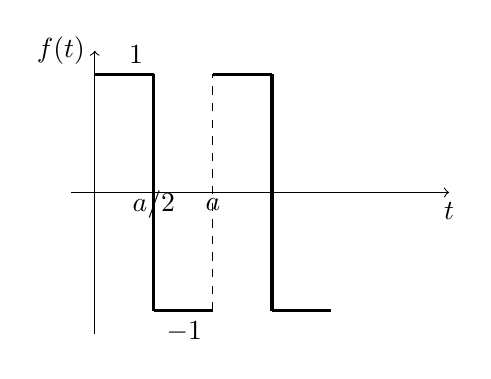
\begin{tikzpicture}[scale=1.5]
			\draw[->] (-0.2,0) -- (3,0) node[below] {$t$};
			\draw[->] (0,-1.2) -- (0,1.2) node[left] {$f(t)$};
			\draw[very thick] (0,1) -- (0.5,1) node[above left] {$1$};
			\draw[very thick] (0.5,1) -- (0.5,-1);
			\draw[very thick] (0.5,-1) -- (1,-1) node[below left] {$-1$};
			\draw[dashed] (1,-1) -- (1,1);
			\draw[very thick] (1,1) -- (1.5,1);
			\draw[very thick] (1.5,1) -- (1.5,-1);
			\draw[very thick] (1.5,-1) -- (2,-1);
			\node at (0.5, -0.1) {$a/2$};
			\node at (1, -0.1) {$a$};
		\end{tikzpicture}
	\end{center}
	\begin{align*}
		F(p) &= \frac{\int_0^a f(t) e^{-pt} dt}{1-e^{-pa}} \\
		\int_0^a f(t) e^{-pt} dt &= \int_0^{a/2} (1) e^{-pt} dt + \int_{a/2}^a (-1) e^{-pt} dt \\
		&= \left[-\frac{1}{p}e^{-pt}\right]_0^{a/2} - \left[-\frac{1}{p}e^{-pt}\right]_{a/2}^a \\
		&= -\frac{1}{p}(e^{-pa/2}-1) + \frac{1}{p}(e^{-pa}-e^{-pa/2}) = \frac{1}{p}(1 - 2e^{-pa/2} + e^{-pa}) = \frac{(1-e^{-pa/2})^2}{p} \\
		F(p) &= \frac{(1-e^{-pa/2})^2}{p(1-e^{-pa})} = \frac{(1-e^{-pa/2})^2}{p(1-e^{-pa/2})(1+e^{-pa/2})} = \frac{1-e^{-pa/2}}{p(1+e^{-pa/2})} \\
		&= \frac{e^{pa/4}-e^{-pa/4}}{p(e^{pa/4}+e^{-pa/4})} = \frac{2\sinh(pa/4)}{p(2\cosh(pa/4))} = \frac{1}{p}\tanh\left(\frac{pa}{4}\right)
	\end{align*}
	
	%====================================================================
	\section*{应用:求解偏微分方程}
	%====================================================================
	
	\subsection*{1. 弦振动方程 (Wave Equation)}
	方程为 $\frac{\partial^2 u}{\partial t^2} = a^2 \frac{\partial^2 u}{\partial x^2}$,其中 $a^2=T/\rho$。
	设初始条件为 $u(x,0) = f(x)$, $u_t(x,0)=g(x)$。对时间 $t$ 进行拉普拉斯变换:
	\begin{align*}
		& \mathcal{L}\left[\frac{\partial^2 u}{\partial t^2}\right] = a^2 \mathcal{L}\left[\frac{\partial^2 u}{\partial x^2}\right] \\
		& p^2 U(x,p) - p u(x,0) - u_t(x,0) = a^2 \frac{d^2 U(x,p)}{dx^2} \\
		& \frac{d^2 U}{dx^2} - \frac{p^2}{a^2}U = -\frac{p}{a^2}f(x) - \frac{1}{a^2}g(x)
	\end{align*}
	这是一个关于 $x$ 的二阶常微分方程。求解 $U(x,p)$ 后再进行拉普拉斯逆变换得到 $u(x,t)$。\\
	对于稳态振动解,可设 $u(x,t)=X(x)e^{i\omega t}$,代入原方程得到亥姆霍兹方程 (Helmholtz equation):
	$$ 
	\frac{d^2 X}{dx^2} + k^2 X = 0, \quad (k=\omega/a) 
	$$
	其通解为 $X(x) = A e^{ikx} + B e^{-ikx}$,代表了沿 x 轴正负方向传播的波。
	
	\subsection*{2. 输电线方程 (Telegrapher's Equation)}
	对于一段微元 $\Delta x$,电压和电流满足:
	\begin{align*}
		& \frac{\partial V}{\partial x} = -RI - L \frac{\partial I}{\partial t} \\
		& \frac{\partial I}{\partial x} = -GV - C \frac{\partial V}{\partial t}
	\end{align*}
	将两式联立消去 $I$,得到关于 $V$ 的电报方程:
	$$ 
	\frac{\partial^2 V}{\partial x^2} = LC \frac{\partial^2 V}{\partial t^2} + (RC+LG) \frac{\partial V}{\partial t} + GRV 
	$$
	\textbf{无损耗情况}: $R=0, G=0$。方程简化为波动方程 $\frac{\partial^2 V}{\partial x^2} = LC \frac{\partial^2 V}{\partial t^2}$。
	\textbf{正弦稳态分析}: 设 $V(x,t) = V(x)e^{i\omega t}$,$I(x,t) = I(x)e^{i\omega t}$。
	\begin{align*}
		& \frac{dV(x)}{dx} = -(R+i\omega L)I(x) = -Z I(x) \\
		& \frac{dI(x)}{dx} = -(G+i\omega C)V(x) = -Y V(x)
	\end{align*}
	其中 $Z, Y$ 分别为串联阻抗和并联导纳。再次微分可得:
	$$ 
	\frac{d^2 V(x)}{dx^2} = ZY \cdot V(x) = \gamma^2 V(x) 
	$$
	其中 $\gamma = \sqrt{ZY} = \sqrt{(R+i\omega L)(G+i\omega C)}$ 称为传播常数。
	$\gamma = \alpha + i\beta$,$\alpha$ 是衰减常数,$\beta$ 是相移常数。
	\textbf{无失真条件}: 为了让信号在传播过程中波形不发生改变,要求相速度 $v_p = \omega/\beta$ 与频率无关。这发生在 $\frac{RC}{LC} = \frac{LG}{LC}$,即 $\frac{R}{L} = \frac{G}{C}$ (Heaviside condition)。
	
	%====================================================================
	\section*{热传导方程}
	%====================================================================
	
	\subsection*{一维杆的热传导方程}
	考虑一维杆,长度为L,截面积为A。
	
	物理量:
	\begin{itemize}
		\item $u(x,t)$: $x$点在$t$时刻的温度
		\item $c$: 比热容
		\item $\rho$: 密度
		\item $Q$: 热量
	\end{itemize}
	
	\textbf{定律:} 单位时间内截面热流量
	$$ 
	Q = -kA \frac{\partial u}{\partial x} 
	$$
	其中$k$是热导率。
	
	考虑$[x, x+\Delta x]$一小段,在$\Delta t$时间内热量变化:
	$$ \Delta Q = Q_1 - Q_2 $$
	$$ Q_1 = -kA \frac{\partial u}{\partial x} \Big|_x \Delta t $$
	$$ Q_2 = -kA \frac{\partial u}{\partial x} \Big|_{x+\Delta x} \Delta t $$
	$$ \Delta Q = c \rho (A \Delta x) \Delta u = c \rho A \Delta x (u(t+\Delta t) - u(t)) $$
	($P=m/V$, $\Delta m = \rho A \Delta x$, 质量守恒)
	$$ \Rightarrow kA \Delta t \left( \frac{\partial u}{\partial x} \Big|_{x+\Delta x} - \frac{\partial u}{\partial x} \Big|_x \right) = c \rho A \Delta x \Delta u $$
	$$ \Rightarrow k \frac{\frac{\partial u}{\partial x} \Big|_{x+\Delta x} - \frac{\partial u}{\partial x} \Big|_x}{\Delta x} = c \rho \frac{\Delta u}{\Delta t} $$
	令$\Delta x, \Delta t \to 0$:
	$$ k \frac{\partial^2 u}{\partial x^2} = c \rho \frac{\partial u}{\partial t} $$
	$$ \frac{\partial u}{\partial t} = a^2 \frac{\partial^2 u}{\partial x^2} \quad (a^2 = \frac{k}{c\rho}) $$
	
	\textbf{热源情形:} 若有热源$f(x,t)$
	$$ 
	\frac{\partial u}{\partial t} = a^2 \frac{\partial^2 u}{\partial x^2} + f(x,t) 
	$$
	若热源由电流产生 $Q_{gen} = I^2 R \Delta t = j^2 \rho_e \delta \Delta x \Delta t$
	$$ Q_1 - Q_2 + Q_{gen} = \Delta Q $$
	$$ kA \Delta t \frac{\partial^2 u}{\partial x^2} \Delta x + j^2 \rho_e \delta \Delta x \Delta t = c \rho \delta \Delta x \Delta u $$
	$$ \Rightarrow \frac{\partial u}{\partial t} = a^2 \frac{\partial^2 u}{\partial x^2} + f $$
	$$ (c\rho \frac{\partial u}{\partial t} = k \frac{\partial^2 u}{\partial x^2} + F) $$
	
	\textbf{例:} 稳定状态 $\frac{\partial u}{\partial t}=0$
	$$ 
	a^2 \frac{\partial^2 u}{\partial x^2} + f = 0 \Rightarrow \frac{\partial^2 u}{\partial x^2} = 0 \quad (\text{若} f=0) 
	$$
	$$ u(x) = Ax + B $$
	
	%====================================================================
	\section*{电磁波方程}
	%====================================================================
	麦克斯韦方程组 ($\rho=0, j=0$ 真空中)
	$$ \nabla \cdot E = 0 $$
	$$ \nabla \cdot B = 0 $$
	$$ \nabla \times E = -\frac{\partial B}{\partial t} $$
	$$ \nabla \times B = \mu_0 \epsilon_0 \frac{\partial E}{\partial t} $$
	其中 $\epsilon_0 \mu_0 = 1/c^2$。
	
	\textbf{推导波动方程:}
	利用恒等式 $\nabla \times (\nabla \times A) = \nabla(\nabla \cdot A) - \Delta A$
	$$ \nabla \times (\nabla \times E) = \nabla(\nabla \cdot E) - \Delta E = -\Delta E $$
	$$ \nabla \times (-\frac{\partial B}{\partial t}) = -\frac{\partial}{\partial t}(\nabla \times B) = -\mu_0 \epsilon_0 \frac{\partial^2 E}{\partial t^2} $$
	$$ \Rightarrow \Delta E = \mu_0 \epsilon_0 \frac{\partial^2 E}{\partial t^2} $$
	$$ \frac{\partial^2 E}{\partial t^2} = c^2 \Delta E $$
	同理对$B$可得
	$$ \frac{\partial^2 B}{\partial t^2} = c^2 \Delta B $$
	
	\textbf{有源情况} ($\rho \neq 0, j \neq 0$)
	$$ \nabla \cdot E = \rho/\epsilon_0 $$
	$$ \nabla \cdot B = 0 $$
	$$ \nabla \times E = -\frac{\partial B}{\partial t} $$
	$$ \nabla \times B = \mu_0 j + \mu_0 \epsilon_0 \frac{\partial E}{\partial t} $$
	$$ \nabla \times (\nabla \times E) = \nabla(\rho/\epsilon_0) - \Delta E = -\frac{\partial}{\partial t}(\mu_0 j + \mu_0 \epsilon_0 \frac{\partial E}{\partial t}) $$
	$$ \Delta E - \mu_0 \epsilon_0 \frac{\partial^2 E}{\partial t^2} = \nabla(\rho/\epsilon_0) + \mu_0 \frac{\partial j}{\partial t} $$
	
	%====================================================================
	\section*{泊松方程}
	%====================================================================
	当$\rho \neq 0, j=0$ (静电场)
	$$ \Delta E = \nabla(\rho/\epsilon_0) $$
	引入电势$\phi$,$E = -\nabla\phi$
	$$ \Delta(-\nabla\phi) = -\nabla(\Delta\phi) = \nabla(\rho/\epsilon_0) $$
	$$ \Delta\phi = -\rho/\epsilon_0 $$
	此为泊松方程。
	无源情形 ($\rho=0$)
	$$ \Delta\phi = 0 $$
	此为拉普拉斯方程。
	
	%====================================================================
	\section*{二阶线性偏微分方程的分类}
	%====================================================================
	考虑方程:
	$$ 
	A \frac{\partial^2 u}{\partial x^2} + 2B \frac{\partial^2 u}{\partial x \partial y} + C \frac{\partial^2 u}{\partial y^2} + D \frac{\partial u}{\partial x} + E \frac{\partial u}{\partial y} + F u = G 
	$$
	其中$A, B, C, D, E, F, G$是$x, y$的函数。
	令 $\Delta = B^2 - AC$
	\begin{itemize}
		\item $\Delta > 0$: 双曲型 (e.g. 波动方程)
		\item $\Delta = 0$: 抛物型 (e.g. 热传导方程)
		\item $\Delta < 0$: 椭圆型 (e.g. 拉普拉斯方程)
	\end{itemize}
	这与二次曲线的分类是类似的。
	
	\textbf{坐标变换}
	令 $\xi = \xi(x,y), \eta = \eta(x,y)$
	$$ \frac{\partial u}{\partial x} = \frac{\partial u}{\partial \xi} \frac{\partial \xi}{\partial x} + \frac{\partial u}{\partial \eta} \frac{\partial \eta}{\partial x} $$
	$$ \frac{\partial u}{\partial y} = \frac{\partial u}{\partial \xi} \frac{\partial \xi}{\partial y} + \frac{\partial u}{\partial \eta} \frac{\partial \eta}{\partial y} $$
	$$ \frac{\partial^2 u}{\partial x^2} = \frac{\partial}{\partial x} (\frac{\partial u}{\partial x}) = \dots $$
	代入原方程,得到新的方程:
	$$ 
	a \frac{\partial^2 u}{\partial \xi^2} + 2b \frac{\partial^2 u}{\partial \xi \partial \eta} + c \frac{\partial^2 u}{\partial \eta^2} + \dots = G 
	$$
	其中
	$$ a = A(\frac{\partial \xi}{\partial x})^2 + 2B \frac{\partial \xi}{\partial x} \frac{\partial \xi}{\partial y} + C(\frac{\partial \xi}{\partial y})^2 $$
	$$ b = A \frac{\partial \xi}{\partial x} \frac{\partial \eta}{\partial x} + B (\frac{\partial \xi}{\partial x} \frac{\partial \eta}{\partial y} + \frac{\partial \xi}{\partial y} \frac{\partial \eta}{\partial x}) + C \frac{\partial \xi}{\partial y} \frac{\partial \eta}{\partial y} $$
	$$ c = A(\frac{\partial \eta}{\partial x})^2 + 2B \frac{\partial \eta}{\partial x} \frac{\partial \eta}{\partial y} + C(\frac{\partial \eta}{\partial y})^2 $$
	可以证明 $b^2 - ac = (B^2 - AC) (\frac{\partial \xi}{\partial x} \frac{\partial \eta}{\partial y} - \frac{\partial \xi}{\partial y} \frac{\partial \eta}{\partial x})^2$
	其中后面的行列式是坐标变换的雅可比行列式。
	
	%====================================================================
	\section*{化为标准型}
	%====================================================================
	目标是选择$\xi, \eta$使得$a,c$中至少一个为0。
	令 $a=0$
	$$ A(\frac{\partial \xi}{\partial x})^2 + 2B \frac{\partial \xi}{\partial x} \frac{\partial \xi}{\partial y} + C(\frac{\partial \xi}{\partial y})^2 = 0 $$
	$$ A \left(\frac{\partial \xi / \partial x}{\partial \xi / \partial y}\right)^2 + 2B \left(\frac{\partial \xi / \partial x}{\partial \xi / \partial y}\right) + C = 0 $$
	根据隐函数定理,沿 $\xi(x,y)=const$ 曲线,有 $\frac{dy}{dx} = - \frac{\partial \xi / \partial x}{\partial \xi / \partial y}$
	$$ A\left(\frac{dy}{dx}\right)^2 - 2B\left(\frac{dy}{dx}\right) + C = 0 $$
	解出 $\frac{dy}{dx}$
	$$ \frac{dy}{dx} = \frac{2B \pm \sqrt{4B^2 - 4AC}}{2A} = \frac{B \pm \sqrt{B^2 - AC}}{A} $$
	这就是特征方程。
	
	\paragraph{(1) $\Delta = B^2 - AC > 0$ (双曲型)}
	有两个不同的实根 $\frac{dy}{dx} = \lambda_1, \frac{dy}{dx} = \lambda_2$。
	解这两个常微分方程,得到两个特征线族 $\phi(x,y) = c_1, \psi(x,y)=c_2$。
	令 $\xi = \phi(x,y), \eta = \psi(x,y)$。
	这样 $a=0, c=0$。方程化为
	$$ 
	2b \frac{\partial^2 u}{\partial \xi \partial \eta} + \dots = 0 \Rightarrow \frac{\partial^2 u}{\partial \xi \partial \eta} = \dots \quad (\text{标准型I}) 
	$$
	若再做变换 $\xi' = \xi+\eta, \eta' = \xi-\eta$,则
	$$ 
	\frac{\partial^2 u}{\partial \xi'^2} - \frac{\partial^2 u}{\partial \eta'^2} = \dots \quad (\text{标准型II}) 
	$$
	
	\paragraph{(2) $\Delta = B^2 - AC = 0$ (抛物型)}
	只有一个实根 $\frac{dy}{dx} = \frac{B}{A}$。
	解得一个特征线族 $\phi(x,y)=c$。
	令 $\xi = \phi(x,y)$,则 $a=0$。
	$\eta$可以任取与$\xi$无关的函数,例如$\eta=x$。
	此时$b=0$, $c \neq 0$。方程化为
	$$ 
	c \frac{\partial^2 u}{\partial \eta^2} = \dots \Rightarrow \frac{\partial^2 u}{\partial \eta^2} = \dots \quad (\text{标准型}) 
	$$
	
	\paragraph{(3) $\Delta = B^2 - AC < 0$ (椭圆型)}
	特征方程的根是共轭复数。
	$$ \frac{dy}{dx} = \frac{B \pm i\sqrt{AC-B^2}}{A} $$
	解也是共轭的,$\phi(x,y) \pm i\psi(x,y) = const$。
	令 $\xi = \phi(x,y), \eta = \psi(x,y)$。
	可以证明 $a=c, b=0$。
	方程化为
	$$ 
	a\left(\frac{\partial^2 u}{\partial \xi^2} + \frac{\partial^2 u}{\partial \eta^2}\right) = \dots \Rightarrow \frac{\partial^2 u}{\partial \xi^2} + \frac{\partial^2 u}{\partial \eta^2} = \dots \quad (\text{标准型}) 
	$$
	
	\subsection*{再探标准型变换}
	\begin{itemize}
		\item[(b)] $\Delta = 0$: (应为 $u_{\eta\eta}=0$)
		取变换
		$$ \xi = x, \quad \eta = y - \frac{B}{A}x $$
		则
		$$ \frac{\partial^2 u}{\partial \xi^2} + \frac{\partial^2 u}{\partial \eta^2} = -\frac{1}{A^2}(\dots) $$
		(笔记此处似有误,应化为 $\frac{\partial^2 u}{\partial \eta^2} = \dots$)
		\item[(c)] $\Delta < 0$: $u_{xx} + u_{yy} = 0$.
		取变换
		$$ \xi = y - \frac{B}{A}x, \quad \eta = \frac{\sqrt{AC-B^2}}{A}x $$
		$$ \Rightarrow \frac{\partial^2 u}{\partial \xi^2} + \frac{\partial^2 u}{\partial \eta^2} = \dots $$
	\end{itemize}
	
	\textbf{总结特征线法:}
	从 $A(\frac{dy}{dx})^2 - 2B(\frac{dy}{dx}) + C = 0$ 出发
	\begin{enumerate}
		\item[(a)] $\Delta > 0$: 两条实特征线
		$$ \frac{dy}{dx} = \frac{B \pm \sqrt{B^2-AC}}{A} $$
		解出 $\phi_1(x,y)=c_1, \phi_2(x,y)=c_2$。
		令 $\xi = \phi_1, \eta = \phi_2$。得标准型:
		$$ \frac{\partial^2 u}{\partial \xi \partial \eta} = d \frac{\partial u}{\partial \xi} + e \frac{\partial u}{\partial \eta} + f u + g $$
		\item[(b)] $\Delta = 0$: 一条实特征线
		$$ \frac{dy}{dx} = \frac{B}{A} $$
		解出 $\phi(x,y)=c$。
		令 $\xi=\phi(x,y)$, $\eta$可任取(如$\eta=x$)。得标准型:
		$$ \frac{\partial^2 u}{\partial \eta^2} = d \frac{\partial u}{\partial \xi} + e \frac{\partial u}{\partial \eta} + f u + g $$
		\item[(c)] $\Delta < 0$: 无实特征线
		取 $\xi = y - \frac{B}{A}x, \eta = \frac{\sqrt{AC-B^2}}{A}x$。得标准型:
		$$ \frac{\partial^2 u}{\partial \xi^2} + \frac{\partial^2 u}{\partial \eta^2} = d \frac{\partial u}{\partial \xi} + e \frac{\partial u}{\partial \eta} + f u + g $$
	\end{enumerate}
	
	\subsection*{例子}
	\begin{enumerate}
		\item $u_{xx} - u_{t t} + a u_t + b u_x = 0$
		$A=1, B=0, C=-1$. $\Delta = 0 - (1)(-1) = 1 > 0$ (双曲型)
		特征方程: $(\frac{dt}{dx})^2 - 1 = 0 \Rightarrow \frac{dt}{dx} = \pm 1$
		特征线: $t-x=c_1, t+x=c_2$
		令 $\xi = x-t, \eta=x+t$.
		
		\item $u_{xx} - 2u_{xt} - u_t = 0$
		$A=1, B=-1, C=0$. $\Delta = (-1)^2 - 0 = 1 > 0$ (双曲型)
		特征方程: $(\frac{dt}{dx})^2 + 2(\frac{dt}{dx}) = 0 \Rightarrow \frac{dt}{dx}( \frac{dt}{dx}+2) = 0$
		$\frac{dt}{dx}=0 \Rightarrow t=c_1$.
		$\frac{dt}{dx}=-2 \Rightarrow t+2x=c_2$.
		令 $\xi = t, \eta=t+2x$.
		
		\item $u_{xx} - 4u_{xy} + 3u_{yy} + 8u_y + x = 0$
		$A=1, B=-2, C=3$. $\Delta = (-2)^2 - 1 \cdot 3 = 1 > 0$ (双曲型)
		
		\item $y u_{xx} + x u_{yy} = 0$
		$A=y, B=0, C=x$. $\Delta = -xy$.
		\begin{itemize}
			\item $xy>0$ (I, III象限): 椭圆型
			\item $xy<0$ (II, IV象限): 双曲型
			\item $x=0$ 或 $y=0$: 抛物型
		\end{itemize}
	\end{enumerate}
	
	%====================================================================
	\section*{定解问题}
	%====================================================================
	
	\subsection*{一维波动方程}
	$$ \begin{cases}
		\frac{\partial^2 u}{\partial t^2} = a^2 \frac{\partial^2 u}{\partial x^2} & 0 < x < L, t>0 \\
		u|_{x=0}=0, u|_{x=L}=0 & \text{(边界条件)} \\
		u|_{t=0}=\phi(x) & \text{(初始位移)} \\
		\frac{\partial u}{\partial t}|_{t=0}=\psi(x) & \text{(初始速度)}
	\end{cases} $$
	
	\textbf{叠加原理:}
	对于线性齐次方程 $L(u)=0$,若 $u_1, u_2$ 是解,则 $c_1 u_1 + c_2 u_2$ 也是解。
	对于 $L(u) = F$ (非齐次方程),其通解为 $u = u_p + u_h$,其中 $u_p$ 是一个特解,$u_h$ 是对应齐次方程的通解。
	此性质可用于分解问题。
	
	\subsection*{一维热传导方程}
	$$ \begin{cases}
		\frac{\partial u}{\partial t} = k \frac{\partial^2 u}{\partial x^2} & 0 < x < L, t>0 \\
		u(0,t)=0, u(L,t)=0 & (t>0) \\
		u(x,0)=f(x) & (0 \le x \le L)
	\end{cases} $$
	这是一个定解问题。
	
	\textbf{例1:稳态解}
	如果边界条件不为零,如 $u(0,t)=T_1, u(L,t)=T_2$。
	稳态解 $u_E(x)$ 满足
	$$ \frac{d^2 u_E}{d x^2} = 0 \Rightarrow u_E(x) = c_1 x + c_2 $$
	代入边界条件
	$$ u_E(0)=T_1 \Rightarrow c_2=T_1 $$
	$$ u_E(L)=T_2 \Rightarrow c_1 L + T_1 = T_2 \Rightarrow c_1 = \frac{T_2-T_1}{L} $$
	所以
	$$ u_E(x) = \frac{T_2-T_1}{L}x + T_1 $$
	令 $u(x,t) = v(x,t) + u_E(x)$,则$v(x,t)$满足齐次边界条件。
	
	\section*{分离变量法 (Separation of Variables Method)}
	\subsection*{弦振动 (String Vibration)}
	
	\noindent The governing partial differential equation (PDE):
	$$ \frac{\partial^2 u}{\partial t^2} = a^2 \frac{\partial^2 u}{\partial x^2} $$
	Initial conditions:
	$$ u|_{t=0} = \phi(x) $$
	$$ \frac{\partial u}{\partial t}\bigg|_{t=0} = \psi(x) $$
	Boundary conditions (fixed ends):
	$$ u|_{x=0} = 0, \quad u|_{x=L} = 0 $$
	Goal: Find the solution $u(x,t)$.
	
	\subsection*{推导 (Derivation)}
	Assume the solution can be written as a product of functions of a single variable:
	$$ u(x,t) = X(x)T(t) $$
	Substitute into the PDE:
	$$ X(x)T''(t) = a^2 X''(x)T(t) $$
	Rearrange the terms to separate variables:
	$$ \frac{X''(x)}{X(x)} = \frac{T''(t)}{a^2 T(t)} $$
	Since the left side depends only on $x$ and the right side only on $t$, both must be equal to a constant. Let's call this constant $-\lambda$.
	$$ \frac{d}{dx}\left[\frac{X''(x)}{X(x)}\right] = 0 $$
	$$ \frac{d}{dt}\left[\frac{T''(t)}{a^2 T(t)}\right] = 0 $$
	This gives two ordinary differential equations (ODEs):
	$$ X''(x) + \lambda X(x) = 0 $$
	$$ T''(t) + \lambda a^2 T(t) = 0 $$
	The boundary conditions for $u(x,t)$ translate to conditions for $X(x)$, since $T(t) \not\equiv 0$ for a non-trivial solution:
	$$ u(0,t) = X(0)T(t) = 0 \implies X(0) = 0 $$
	$$ u(L,t) = X(L)T(t) = 0 \implies X(L) = 0 $$
	
	\subsection*{求解本征值问题 (Solving the Eigenvalue Problem for X(x))}
	We analyze the possible values of the separation constant $\lambda$.
	
	\paragraph{Case 1: $\lambda = 0$}
	The equation for $X(x)$ is $X''(x) = 0$.
	The general solution is:
	$$ X(x) = Ax + B $$
	Applying the boundary conditions:
	$$ X(0) = B = 0 $$
	$$ X(L) = AL + B = 0 \implies A = 0 $$
	This gives $X(x) = 0$, which leads to the trivial solution $u(x,t) = 0$.
	
	\paragraph{Case 2: $\lambda < 0$}
	Let $\lambda = -k^2$ where $k > 0$. The equation is $X''(x) - k^2 X(x) = 0$.
	The general solution is:
	$$ X(x) = A \cosh(kx) + B \sinh(kx) $$
	Applying the boundary conditions:
	$$ X(0) = A \cosh(0) + B \sinh(0) = A = 0 $$
	$$ X(L) = B \sinh(kL) = 0 $$
	Since $k>0$ and $L>0$, $\sinh(kL) \neq 0$, so $B=0$.
	This again leads to the trivial solution $X(x) = 0$.
	
	\paragraph{Case 3: $\lambda > 0$}
	Let $\lambda = k^2$ where $k > 0$. The equation is $X''(x) + k^2 X(x) = 0$.
	The general solution is:
	$$ X(x) = A \cos(kx) + B \sin(kx) $$
	Applying the boundary conditions:
	$$ X(0) = A \cos(0) + B \sin(0) = A = 0 $$
	So,
	$$ X(x) = B \sin(kx) $$
	$$ X(L) = B \sin(kL) = 0 $$
	For a non-trivial solution, we must have $B \neq 0$, which implies:
	$$ \sin(kL) = 0 $$
	This means $kL = n\pi$ for $n = 1, 2, 3, \dots$.
	The possible values for $k$ are:
	$$ k_n = \frac{n\pi}{L} $$
	These lead to the eigenvalues (本征值):
	$$ \lambda_n = k_n^2 = \left(\frac{n\pi}{L}\right)^2 $$
	The corresponding eigenfunctions (本征函数) are:
	$$ X_n(x) = B_n \sin\left(\frac{n\pi x}{L}\right) $$
	
	\subsection*{求解 T(t) 并叠加 (Solving for T(t) and Superposition)}
	Now we solve for $T(t)$ using the found eigenvalues $\lambda_n$:
	$$ T_n''(t) + \lambda_n a^2 T_n(t) = 0 $$
	$$ T_n''(t) + \left(\frac{n\pi a}{L}\right)^2 T_n(t) = 0 $$
	The general solution for $T_n(t)$ is:
	$$ T_n(t) = C_n \cos\left(\frac{n\pi a t}{L}\right) + D_n \sin\left(\frac{n\pi a t}{L}\right) $$
	The solution for each mode $n$ is $u_n(x,t) = X_n(x) T_n(t)$. We absorb the constant $B_n$ into $C_n$ and $D_n$.
	$$ u_n(x,t) = \left(C_n \cos\left(\frac{n\pi a t}{L}\right) + D_n \sin\left(\frac{n\pi a t}{L}\right)\right) \sin\left(\frac{n\pi x}{L}\right) $$
	By the superposition principle (叠加原理), the general solution is the sum of all possible solutions:
	$$ u(x,t) = \sum_{n=1}^{\infty} u_n(x,t) $$
	$$ u(x,t) = \sum_{n=1}^{\infty} \left(C_n \cos\left(\frac{n\pi a t}{L}\right) + D_n \sin\left(\frac{n\pi a t}{L}\right)\right) \sin\left(\frac{n\pi x}{L}\right) $$
	
	\subsection*{利用初始条件 (Using Initial Conditions)}
	We determine the coefficients $C_n$ and $D_n$ using the initial conditions.
	At $t=0$:
	$$ u(x,0) = \phi(x) = \sum_{n=1}^{\infty} C_n \sin\left(\frac{n\pi x}{L}\right) $$
	This is a Fourier sine series for $\phi(x)$. The coefficients $C_n$ are given by:
	$$ C_n = \frac{2}{L} \int_0^L \phi(x) \sin\left(\frac{n\pi x}{L}\right) dx $$
	Next, we find the derivative with respect to $t$:
	$$ \frac{\partial u}{\partial t} = \sum_{n=1}^{\infty} \left(-C_n \frac{n\pi a}{L} \sin\left(\frac{n\pi a t}{L}\right) + D_n \frac{n\pi a}{L} \cos\left(\frac{n\pi a t}{L}\right)\right) \sin\left(\frac{n\pi x}{L}\right) $$
	At $t=0$:
	$$ \frac{\partial u}{\partial t}\bigg|_{t=0} = \psi(x) = \sum_{n=1}^{\infty} D_n \frac{n\pi a}{L} \sin\left(\frac{n\pi x}{L}\right) $$
	This is a Fourier sine series for $\psi(x)$. The coefficients are given by:
	$$ D_n \frac{n\pi a}{L} = \frac{2}{L} \int_0^L \psi(x) \sin\left(\frac{n\pi x}{L}\right) dx $$
	$$ D_n = \frac{2}{n\pi a} \int_0^L \psi(x) \sin\left(\frac{n\pi x}{L}\right) dx $$
	
	\subsection*{分离变量法总结 (Summary of Separation of Variables)}
	\begin{enumerate}
		\item \textbf{分离变量:} 设定 $u=TX$ (Let $u=TX$)
		\item \textbf{定解:} 代入得 $X(x), T(t)$ 常微分方程 (Substitute to get ODEs for $X(x), T(t)$)
		\item \textbf{边界条件:} 求解 $X(x)$, 边界条件 (齐次) $\implies$ 本征值 $\lambda_n$ 与本征函数 $X_n(x)$ (Solve for $X(x)$ using homogeneous boundary conditions to get eigenvalues $\lambda_n$ and eigenfunctions $X_n(x)$)
		\item \textbf{齐次:} 代入 $\lambda_n \to T_n(t)$ (Substitute $\lambda_n$ to find $T_n(t)$)
		\item \textbf{叠加原理:} $u(x,t) = \sum u_n(x,t)$ (Superposition principle)
	\end{enumerate}
	
	\section*{基本解问题 (Examples of Fundamental Solutions)}
	\subsection*{例1 (Example 1: Plucked String)}
	Problem:
	$$ \frac{\partial^2 u}{\partial t^2} = a^2 \frac{\partial^2 u}{\partial x^2} $$
	$$ u(x,0) = \phi(x) = \begin{cases} \frac{3}{2}x & 0 \le x \le 2/5 \\ 3(1-x) & 2/5 \le x \le 1 \end{cases} \quad (\text{with } L=1) $$
	$$ \frac{\partial u}{\partial t}\bigg|_{t=0} = \psi(x) = 0 $$
	$$ u(0,t) = 0, \quad u(1,t) = 0 $$
	Since $\psi(x)=0$, we have $D_n=0$ for all $n$.
	We calculate $C_n$:
	$$ C_n = \frac{2}{1} \int_0^1 \phi(x) \sin(n\pi x) dx $$
	$$ C_n = 2 \left[ \int_0^{2/5} \frac{3}{2}x \sin(n\pi x) dx + \int_{2/5}^1 3(1-x) \sin(n\pi x) dx \right] $$
	After integration (result from notes):
	$$ C_n = \frac{9}{5n^2\pi^2} \sin\left(\frac{2n\pi}{5}\right) $$
	The final solution is:
	$$ u(x,t) = \sum_{n=1}^{\infty} \frac{9}{5n^2\pi^2} \sin\left(\frac{2n\pi}{5}\right) \cos(n\pi at) \sin(n\pi x) $$
	
	\subsection*{例2 (Example 2: Struck String)}
	Problem:
	$$ \frac{\partial^2 u}{\partial t^2} = a^2 \frac{\partial^2 u}{\partial x^2} $$
	$$ u(x,0) = \phi(x) = 0 $$
	$$ \frac{\partial u}{\partial t}\bigg|_{t=0} = \psi(x) = \frac{K}{\rho}\delta(x-c) \quad (\text{impulse at } x=c) $$
	$$ u(0,t) = 0, \quad u(L,t) = 0 $$
	Since $\phi(x)=0$, we have $C_n = 0$ for all $n$.
	We calculate $D_n$:
	$$ D_n = \frac{2}{n\pi a} \int_0^L \psi(x) \sin\left(\frac{n\pi x}{L}\right) dx $$
	$$ D_n = \frac{2}{n\pi a} \int_0^L \frac{K}{\rho} \delta(x-c) \sin\left(\frac{n\pi x}{L}\right) dx $$
	Using the sifting property of the Dirac delta function:
	$$ D_n = \frac{2K}{n\pi a \rho} \sin\left(\frac{n\pi c}{L}\right) $$
	The final solution is:
	$$ u(x,t) = \sum_{n=1}^{\infty} \frac{2K}{n\pi a \rho} \sin\left(\frac{n\pi c}{L}\right) \sin\left(\frac{n\pi a t}{L}\right) \sin\left(\frac{n\pi x}{L}\right) $$
	
	\section*{物理解释 (Physical Interpretation)}
	The solution for a single mode can be written in phase-amplitude form:
	$$ u_n(x,t) = N_n \sin(\omega_n t + \theta_n) \sin\left(\frac{n\pi x}{L}\right) $$
	where the angular frequency is $\omega_n = \frac{n\pi a}{L}$.
	The amplitude $N_n$ and phase $\theta_n$ are given by:
	$$ N_n = \sqrt{C_n^2+D_n^2} $$
	$$ \tan\theta_n = \frac{C_n}{D_n} $$
	An alternative form from the notes is:
	$$ u_n(x,t) = A_n(t) \sin\left(\frac{n\pi x}{L}\right) $$
	$$ u_n(t) = B_n(x_0) \sin(\omega_n t + \theta_n) $$
	
	\subsection*{驻波 (Standing Waves)}
	The solution $u_n(x,t)$ represents a standing wave.
	\begin{itemize}
		\item \textbf{节点 (Nodes):} Points that do not move. Occur when $\sin(\frac{n\pi x}{L}) = 0$.
		$$ \frac{n\pi x}{L} = m\pi, \quad m = 0, 1, \dots, n $$
		$$ x_m = \frac{m}{n}L $$
		\item \textbf{波腹 (Antinodes):} Points of maximum amplitude ($x_0$).
	\end{itemize}
	
	\subsection*{单模振动 (Single-mode Oscillation)}
	A single eigenfunction corresponds to a single mode of vibration.
	$$ E \sim \sin\left(\frac{n\pi x}{L}\right) $$
	
	\subsection*{与量子力学类比 (Analogy to Quantum Mechanics)}
	The spatial part of the wave solution is analogous to the wave function for a particle in a 1D infinite potential well.
	$$ \Psi \sim \sin\left(\frac{n\pi x}{L}\right) $$
	The time-dependent Schrödinger equation:
	$$ i\hbar \frac{\partial \Psi}{\partial t} = -\frac{\hbar^2}{2m} \nabla^2 \Psi + U(x)\Psi $$
	
	\section*{其他边界条件 (Other Boundary Conditions)}
	\begin{enumerate}
		\item \textbf{两端固定 (Fixed-Fixed):} $u(0,t)=0$, $u(L,t)=0$.
		\item \textbf{一端固定, 一端自由 (Fixed-Free):} $u(0,t)=0$, $\frac{\partial u}{\partial x}\bigg|_{x=L}=0$.
		\item \textbf{两端自由 (Free-Free):} $\frac{\partial u}{\partial x}\bigg|_{x=0}=0$, $\frac{\partial u}{\partial x}\bigg|_{x=L}=0$.
		\item \textbf{辐射边界条件 (Radiation Boundary Condition):} $-k\frac{\partial u}{\partial x}\bigg|_{x=L} = H(u(L,t) - u_0)$.
	\end{enumerate}
	
	\section*{有阻尼波动方程与电报方程 (Damped Wave and Telegrapher's Equation)}
	
	\subsection*{例: 电报方程 (Example: Telegrapher's Equation)}
	The general form of the Telegrapher's equation is:
	$$ \frac{\partial^2 u}{\partial t^2} - a^2 \frac{\partial^2 u}{\partial x^2} + 2b \frac{\partial u}{\partial t} + c u = 0 $$
	With initial conditions:
	$$ u|_{t=0} = \phi(x) $$
	$$ \frac{\partial u}{\partial t}\bigg|_{t=0} = \psi(x) $$
	And boundary conditions ($b, c > 0$):
	$$ u|_{x=0} = 0, \quad u|_{x=L} = 0 $$
	Using separation of variables, $u(x,t) = X(x)T(t)$, we get:
	$$ X''(x) + \lambda X(x) = 0 $$
	$$ X(0) = 0, \quad X(L) = 0 $$
	and
	$$ T''(t) + 2b T'(t) + (\lambda a^2 + c) T(t) = 0 $$
	The solution for $X(x)$ is the same as for the standard wave equation:
	$$ \lambda_n = \left(\frac{n\pi}{L}\right)^2 $$
	$$ X_n(x) = B_n \sin\left(\frac{n\pi x}{L}\right) $$
	The solution for $T(t)$ is that of a damped harmonic oscillator. For the underdamped case, the solution has the form:
	$$ u(x,t) = e^{-bt} \sum_{n=1}^{\infty} \left(C_n \cos(q_n t) + D_n \sin(q_n t)\right) \sin\left(\frac{n\pi x}{L}\right) $$
	where the new frequency $q_n$ is:
	$$ q_n = \sqrt{\left|\left(\frac{n\pi a}{L}\right)^2 + c - b^2\right|} $$
	The coefficients $C_n, D_n$ are determined by the initial conditions.
	
	\subsection*{例: 有阻尼波动方程 (Example: Damped Wave Equation)}
	This is a special case of the Telegrapher's equation where $c=0$.
	$$ \frac{\partial^2 u}{\partial t^2} - a^2 \frac{\partial^2 u}{\partial x^2} + 2b \frac{\partial u}{\partial t} = 0 $$
	The equation for $T(t)$ becomes:
	$$ T_n''(t) + 2b T_n'(t) + \lambda_n a^2 T_n(t) = 0 $$
	The characteristic equation is $r^2 + 2br + (\frac{n\pi a}{L})^2 = 0$. The behavior depends on the discriminant. Let $q_n = \sqrt{\left| (\frac{n\pi a}{L})^2 - b^2 \right|}$.
	
	The general solution for $T_n(t)$ can be one of three cases for each mode $n$:
	\begin{enumerate}
		\item \textbf{Underdamped} ($\frac{n\pi a}{L} > b$):
		$$ T_n(t) = e^{-bt} \left(C_n \cos(q_n t) + D_n \sin(q_n t)\right) $$
		\item \textbf{Critically Damped} ($\frac{n\pi a}{L} = b$):
		$$ T_n(t) = e^{-bt} (C_n + D_n t) $$
		\item \textbf{Overdamped} ($\frac{n\pi a}{L} < b$):
		$$ T_n(t) = e^{-bt} \left(C_n \cosh(q_n t) + D_n \sinh(q_n t)\right) $$
	\end{enumerate}
	Let's assume the underdamped case holds for all modes of interest ($\frac{bL}{\pi a} < 1$). The total solution is:
	$$ u(x,t) = \sum_{n=1}^{\infty} e^{-bt} \left(C_n \cos(q_n t) + D_n \sin(q_n t)\right) \sin\left(\frac{n\pi x}{L}\right) $$
	To find the coefficients from $u(x,0) = \phi(x)$ and $u_t(x,0)=\psi(x)$:
	$$ \phi(x) = \sum_{n=1}^{\infty} C_n \sin\left(\frac{n\pi x}{L}\right) $$
	$$ \implies C_n = \frac{2}{L} \int_0^L \phi(x) \sin\left(\frac{n\pi x}{L}\right) dx $$
	$$ \psi(x) = \sum_{n=1}^{\infty} (-b C_n + q_n D_n) \sin\left(\frac{n\pi x}{L}\right) $$
	$$ \implies -b C_n + q_n D_n = \frac{2}{L} \int_0^L \psi(x) \sin\left(\frac{n\pi x}{L}\right) dx $$
	$$ \implies D_n = \frac{b}{q_n} C_n + \frac{2}{q_n L} \int_0^L \psi(x) \sin\left(\frac{n\pi x}{L}\right) dx $$
	If the initial velocity is zero, $\psi(x)=0$, then $D_n = \frac{b}{q_n}C_n$.
	
	\newpage
	\section*{热传导方程 (Heat Equation)}
	\subsection*{例: 傅里叶热棒 (Example: Fourier Heat Rod)}
	The problem describes the temperature $u(x,t)$ in a rod with insulated ends.
	$$ \frac{\partial u}{\partial t} = a^2 \frac{\partial^2 u}{\partial x^2} $$
	Initial condition:
	$$ u(t=0) = \phi(x) $$
	Boundary conditions (insulated ends):
	$$ \frac{\partial u}{\partial x}\bigg|_{x=0} = 0, \quad \frac{\partial u}{\partial x}\bigg|_{x=L} = 0 $$
	Separating variables $u(x,t) = X(x)T(t)$ yields:
	$$ X''(x) + \lambda X(x) = 0, \quad \text{with } X'(0)=0, X'(L)=0 $$
	$$ T'(t) + \lambda a^2 T(t) = 0 $$
	Solving the eigenvalue problem for $X(x)$:
	\begin{itemize}
		\item Case $\lambda=0$: $X''(x)=0 \implies X(x) = Ax+B$. $X'(0)=A=0$. $X'(L)=A=0$. So $X_0(x) = B_0$ (a constant) is an eigenfunction.
		\item Case $\lambda < 0$: Trivial solution $X(x)=0$.
		\item Case $\lambda > 0$ ($\lambda=k^2$): $X(x) = A\cos(kx)+B\sin(kx)$. $X'(0) = B k = 0 \implies B=0$. $X'(L) = -A k \sin(kL) = 0 \implies \sin(kL)=0$. Thus $kL=n\pi$ for $n=1,2,3,\dots$.
	\end{itemize}
	The eigenvalues are $\lambda_n = (\frac{n\pi}{L})^2$ for $n=0, 1, 2, \dots$.
	The eigenfunctions are $X_n(x) = A_n \cos(\frac{n\pi x}{L})$.
	Solving for $T(t)$:
	For $n>0$: $T_n'(t) + (\frac{n\pi a}{L})^2 T_n(t) = 0 \implies T_n(t) = C_n e^{-(\frac{n\pi a}{L})^2 t}$.
	For $n=0$ ($\lambda_0=0$): $T_0'(t)=0 \implies T_0(t) = C_0$.
	The general solution is by superposition:
	$$ u(x,t) = C_0 + \sum_{n=1}^{\infty} C_n \exp\left[-\left(\frac{n\pi a}{L}\right)^2 t\right] \cos\left(\frac{n\pi x}{L}\right) $$
	Using the initial condition $u(x,0)=\phi(x)$:
	$$ \phi(x) = C_0 + \sum_{n=1}^{\infty} C_n \cos\left(\frac{n\pi x}{L}\right) $$
	This is a Fourier cosine series. The coefficients are:
	$$ C_0 = \frac{1}{L} \int_0^L \phi(x) dx $$
	$$ C_n = \frac{2}{L} \int_0^L \phi(x) \cos\left(\frac{n\pi x}{L}\right) dx $$
	
	\newpage
	\section*{波动方程更多示例 (Further Examples for the Wave Equation)}
	\subsection*{例: 自由-固定端 (Example: Free-Fixed End)}
	The note appears to solve for a rod with a free end at $x=0$ and a fixed end at $x=L$.
	$$ \frac{\partial^2 u}{\partial t^2} = a^2 \frac{\partial^2 u}{\partial x^2} $$
	$$ \frac{\partial u}{\partial x}\bigg|_{x=0}=0, \quad u|_{x=L}=0 $$
	Separation of variables leads to $X''(x)+\lambda X(x)=0$ with $X'(0)=0, X(L)=0$.
	Let $\lambda=k^2$. $X(x)=A\cos(kx)+B\sin(kx)$.
	$$ X'(0) = B k = 0 \implies B=0 $$
	$$ X(L) = A\cos(kL) = 0 \implies kL = \frac{(2n+1)\pi}{2}, \quad n=0, 1, 2, \dots $$
	The eigenvalues and eigenfunctions are:
	$$ \lambda_n = \left(\frac{(2n+1)\pi}{2L}\right)^2 $$
	$$ X_n(x) = A_n \cos\left(\frac{(2n+1)\pi x}{2L}\right) $$
	The general solution is:
	$$ u(x,t) = \sum_{n=0}^{\infty} \left(C_n \cos\left(\frac{(2n+1)\pi a t}{2L}\right) + D_n \sin\left(\frac{(2n+1)\pi a t}{2L}\right)\right) \cos\left(\frac{(2n+1)\pi x}{2L}\right) $$
	Coefficients are found from initial conditions $\phi(x)$ and $\psi(x)$:
	$$ C_n = \frac{2}{L} \int_0^L \phi(x) \cos\left(\frac{(2n+1)\pi x}{2L}\right) dx $$
	$$ D_n = \frac{2}{L} \frac{2L}{(2n+1)\pi a} \int_0^L \psi(x) \cos\left(\frac{(2n+1)\pi x}{2L}\right) dx $$
	\paragraph{Specific Case:} If $u(x,0) = \cos(\frac{\pi x}{2L})$ and $u_t(x,0)=0$.
	This corresponds to the $n=0$ mode.
	$$ D_n = 0 \text{ for all } n $$
	$$ C_n = \frac{2}{L} \int_0^L \cos\left(\frac{\pi x}{2L}\right) \cos\left(\frac{(2n+1)\pi x}{2L}\right) dx $$
	By orthogonality, this integral is non-zero only for $n=0$.
	$$ C_0 = \frac{2}{L} \int_0^L \cos^2\left(\frac{\pi x}{2L}\right) dx = \frac{2}{L} \cdot \frac{L}{2} = 1 $$
	All other $C_n=0$. The solution is:
	$$ u(x,t) = \cos\left(\frac{\pi a t}{2L}\right) \cos\left(\frac{\pi x}{2L}\right) $$
	
	\subsection*{例: 固定-自由端 (Example: Fixed-Free End)}
	Another example shows fixed-free boundary conditions: $u(0,t)=0, u_x(L,t)=0$.
	Eigenfunctions: $\sin(\frac{(2n+1)\pi x}{2L})$.
	Initial conditions: $u(x,0)=E$ (a constant), $u_t(x,0)=0$.
	Then $D_n=0$ for all $n$.
	$$ C_n = \frac{2}{L} \int_0^L E \sin\left(\frac{(2n+1)\pi x}{2L}\right) dx $$
	$$ C_n = \frac{2E}{L} \left[-\frac{2L}{(2n+1)\pi} \cos\left(\frac{(2n+1)\pi x}{2L}\right) \right]_0^L $$
	$$ C_n = -\frac{4E}{(2n+1)\pi} (\cos(\frac{(2n+1)\pi}{2}) - \cos(0)) = \frac{4E}{(2n+1)\pi} $$
	The solution is:
	$$ u(x,t) = \frac{4E}{\pi} \sum_{n=0}^{\infty} \frac{1}{2n+1} \cos\left(\frac{(2n+1)\pi a t}{2L}\right) \sin\left(\frac{(2n+1)\pi x}{2L}\right) $$
	总结 (Summary)
	$$
	X''(x) + \lambda X(x) = 0
	$$
	$$
	u|_{x=0} = u|_{x=L} = 0 \quad \Rightarrow \quad \lambda_n = (\frac{n\pi}{L})^2, \quad X_n(x) = B_n \sin(\frac{n\pi x}{L})
	$$
	$$
	\frac{\partial u}{\partial x}|_{x=0} = \frac{\partial u}{\partial x}|_{x=L} = 0 \quad \Rightarrow \quad \lambda_n = (\frac{n\pi}{L})^2, \quad X_n(x) = A_n \cos(\frac{n\pi x}{L})
	$$
	$$
	u|_{x=0} = \frac{\partial u}{\partial x}|_{x=L} = 0 \quad \Rightarrow \quad \lambda_n = (\frac{(2n+1)\pi}{2L})^2, \quad X_n(x) = A_n \cos(\frac{(2n+1)\pi x}{2L})
	$$
	
	二维波动方程 (2D Wave Equation)
	$$
	\frac{\partial^2 u}{\partial t^2} = c^2 (\frac{\partial^2 u}{\partial x^2} + \frac{\partial^2 u}{\partial y^2})
	$$
	$$
	\begin{cases}
		u|_{t=0} = \phi(x,y) \\
		u_t|_{t=0} = \psi(x,y) \\
		u|_{x=0} = u|_{x=a} = 0 \quad 0 \le y \le b \\
		u|_{y=0} = u|_{y=b} = 0 \quad 0 \le x \le a
	\end{cases}
	$$
	令 (Let)
	$$
	u(x,y,t) = V(x,y)T(t)
	$$
	$$
	\Rightarrow \frac{T''}{c^2 T} = \frac{1}{V}(\frac{\partial^2 V}{\partial x^2} + \frac{\partial^2 V}{\partial y^2}) = -\lambda
	$$
	$$
	\Rightarrow \frac{\partial^2 V}{\partial x^2} + \frac{\partial^2 V}{\partial y^2} + \lambda V = 0
	$$
	$$
	T'' + \lambda c^2 T = 0
	$$
	再令 (Let again)
	$$
	V(x,y) = X(x)Y(y)
	$$
	$$
	\Rightarrow \frac{X''}{X} = -\frac{Y''+\lambda Y}{Y} = -\mu
	$$
	$$
	\Rightarrow \begin{cases}
		X''+\mu X=0 \\
		X(0)=X(a)=0
	\end{cases}
	$$
	$$
	\begin{cases}
		Y''+\nu Y=0, \quad \nu = \lambda - \mu \\
		Y(0)=Y(b)=0
	\end{cases}
	$$
	解得 (Solution is)
	$$
	\mu_m = (\frac{m\pi}{a})^2, \quad X_m(x) = \sin(\frac{m\pi x}{a})
	$$
	$$
	\nu_n = (\frac{n\pi}{b})^2, \quad Y_n(y) = \sin(\frac{n\pi y}{b})
	$$
	到 (Thus)
	$$
	\lambda_{mn} = (\frac{m\pi}{a})^2 + (\frac{n\pi}{b})^2
	$$
	$$
	V_{mn}(x,y) = \sin(\frac{m\pi x}{a}) \sin(\frac{n\pi y}{b})
	$$
	代入 (Substitute into T)
	$$
	T_{mn}(t) = C_{mn} \cos(\omega_{mn} t) + D_{mn} \sin(\omega_{mn} t)
	$$
	$$
	\omega_{mn} = c \sqrt{\lambda_{mn}} = c\pi \sqrt{(\frac{m}{a})^2 + (\frac{n}{b})^2}
	$$
	基频 (Fundamental frequency)
	$$
	\omega_{11} = c\pi \sqrt{\frac{1}{a^2} + \frac{1}{b^2}}
	$$
	叠加 (Superposition)
	$$
	u(x,y,t) = \sum_{m=1}^{\infty} \sum_{n=1}^{\infty} u_{mn}(x,y,t) = \sum_{m=1}^{\infty} \sum_{n=1}^{\infty} (C_{mn} \cos(\omega_{mn} t) + D_{mn} \sin(\omega_{mn} t)) \sin(\frac{m\pi x}{a})\sin(\frac{n\pi y}{b})
	$$
	$$
	\phi(x,y) = \sum_{m=1}^{\infty} \sum_{n=1}^{\infty} C_{mn} \sin(\frac{m\pi x}{a})\sin(\frac{n\pi y}{b})
	$$
	$$
	\psi(x,y) = \sum_{m=1}^{\infty} \sum_{n=1}^{\infty} \omega_{mn} D_{mn} \sin(\frac{m\pi x}{a})\sin(\frac{n\pi y}{b})
	$$
	正交性 (Orthogonality)
	$$
	\int_0^a \int_0^b V_{mn}(x,y) V_{m'n'}(x,y) dx dy = (\int_0^a \sin(\frac{m\pi x}{a})\sin(\frac{m'\pi x}{a}) dx)(\int_0^b \sin(\frac{n\pi y}{b})\sin(\frac{n'\pi y}{b}) dy)
	$$
	$$
	= \frac{ab}{4} \delta_{mm'} \delta_{nn'}
	$$
	得 (We get)
	$$
	C_{mn} = \frac{4}{ab} \int_0^a \int_0^b \phi(x,y) \sin(\frac{m\pi x}{a})\sin(\frac{n\pi y}{b}) dx dy
	$$
	$$
	D_{mn} = \frac{4}{ab \omega_{mn}} \int_0^a \int_0^b \psi(x,y) \sin(\frac{m\pi x}{a})\sin(\frac{n\pi y}{b}) dx dy
	$$
	特征函数集 (Set of eigenfunctions)
	$$
	\{ \sin(\frac{m\pi x}{a}) \sin(\frac{n\pi y}{b}) \}
	$$
	例 (Example)
	$$
	a=b=1, \quad c = \frac{1}{\pi}
	$$
	$$
	\phi = x(1-x)y(1-y)
	$$
	$$
	\psi = 0 \quad \Rightarrow \quad D_{mn}=0
	$$
	$$
	C_{mn} = 4 \int_0^1 \int_0^1 x(1-x)y(1-y) \sin(m\pi x)\sin(n\pi y) dx dy
	$$
	$$
	= 4 [\int_0^1 x(1-x) \sin(m\pi x) dx] [\int_0^1 y(1-y) \sin(n\pi y) dy]
	$$
	$$
	\int_0^1 x(1-x) \sin(m\pi x) dx = \frac{2(1-(-1)^m)}{m^3\pi^3}
	$$
	$$
	C_{mn} = 4 \frac{2(1-(-1)^m)}{m^3\pi^3} \frac{2(1-(-1)^n)}{n^3\pi^3} = \frac{16(1-(-1)^m)(1-(-1)^n)}{m^3 n^3 \pi^6}
	$$
	解 (Solution)
	$$
	u = \sum_{m,n=1,3,5,...}^{\infty} \frac{64}{\pi^6 m^3 n^3} \cos(\sqrt{m^2+n^2}t) \sin(m\pi x)\sin(n\pi y)
	$$
	
	二维热传导方程 (2D Heat Equation)
	$$
	\frac{\partial u}{\partial t} = c^2 (\frac{\partial^2 u}{\partial x^2} + \frac{\partial^2 u}{\partial y^2})
	$$
	$$
	u|_{t=0} = \phi(x,y)
	$$
	$$
	u|_{x=0}=u|_{x=a}=0, \quad u|_{y=0}=u|_{y=b}=0
	$$
	令 (Let)
	$$
	u=V(x,y)T(t)
	$$
	$$
	\Rightarrow \frac{1}{c^2 T} \frac{\partial T}{\partial t} = \frac{1}{V}(\frac{\partial^2 V}{\partial x^2} + \frac{\partial^2 V}{\partial y^2}) = -\lambda
	$$
	$$
	\Rightarrow \frac{\partial^2 V}{\partial x^2} + \frac{\partial^2 V}{\partial y^2} + \lambda V = 0
	$$
	$$
	T' + c^2 \lambda T = 0
	$$
	$$
	\Rightarrow \lambda_{mn} = (\frac{m\pi}{a})^2 + (\frac{n\pi}{b})^2
	$$
	$$
	V_{mn}(x,y) = \sin(\frac{m\pi x}{a})\sin(\frac{n\pi y}{b})
	$$
	$$
	T_{mn}(t) = e^{- \omega_{mn} t}
	$$
	$$
	\omega_{mn} = c^2 \lambda_{mn} = c^2\pi^2 ((\frac{m}{a})^2+(\frac{n}{b})^2)
	$$
	解 (Solution)
	$$
	u = \sum_{m=1}^{\infty} \sum_{n=1}^{\infty} C_{mn} e^{-\omega_{mn}t} \sin(\frac{m\pi x}{a})\sin(\frac{n\pi y}{b})
	$$
	$$
	C_{mn} = \frac{4}{ab} \int_0^a \int_0^b \phi(x,y) \sin(\frac{m\pi x}{a})\sin(\frac{n\pi y}{b}) dx dy
	$$
	
	例1 (Example 1)
	$$
	a=b=1, c=1
	$$
	$$
	\phi = x(1-x)y(1-y)
	$$
	解 (Solution)
	$$
	u(x,y,t) = \sum_{m,n=1,3,5,...}^{\infty} \frac{64}{m^3 n^3 \pi^6} e^{-[ (m\pi)^2 + (n\pi)^2 ]t} \sin(m\pi x)\sin(n\pi y)
	$$
	中心温度 (Temperature at the center)
	$$
	u(\frac{1}{2}, \frac{1}{2}, t) = \sum_{m,n=1,3,5,...}^{\infty} \frac{64}{m^3 n^3 \pi^6} e^{-[ (m\pi)^2 + (n\pi)^2 ]t} \sin(\frac{m\pi}{2})\sin(\frac{n\pi}{2})
	$$
	
	例2 (Example 2)
	$$
	a=b=1, c=1
	$$
	$$
	\phi = \sin(\pi x) \sin(\pi y)
	$$
	解 (Solution)
	$$
	C_{mn} = 4 \int_0^1 \int_0^1 \sin(\pi x)\sin(\pi y) \sin(m\pi x)\sin(n\pi y) dx dy
	$$
	$$
	= \delta_{m1} \delta_{n1}
	$$
	$$
	u = \sum_{m=1}^{\infty} \sum_{n=1}^{\infty} \delta_{m1} \delta_{n1} e^{-\omega_{mn}t} \sin(m\pi x)\sin(n\pi y)
	$$
	$$
	u = e^{-2\pi^2 t} \sin(\pi x)\sin(\pi y)
	$$
	$$
	u(\frac{1}{2}, \frac{1}{2}, t) = e^{-2\pi^2 t}
	$$
	
	一维热传导方程相关 (Related 1D Heat Equation Concepts)
	(a) 稳态温度 (Steady-state temperature) ($t \to \infty$)
	$$
	u(x, \infty) = C_0 = \frac{1}{L} \int_0^L \phi(x) dx
	$$
	$$
	u(x, 0) = \phi(x) \quad u(x, \infty) = \text{常数} (\text{constant})
	$$
	平均温度 (Average temperature)
	$$
	U(t) = \frac{1}{L} \int_0^L u(x,t) dx = C_0
	$$
	(b) 若 (If) $\phi(x)=x$:
	$$
	C_0 = \frac{L}{2}
	$$
	$$
	C_n = \frac{2}{L} \int_0^L x \cos(\frac{n\pi x}{L}) dx = \frac{2L}{n^2\pi^2}[(-1)^n - 1]
	$$
	$$
	u(x,t) = \frac{L}{2} + \sum_{n=1}^{\infty} \frac{2L}{n^2\pi^2}[(-1)^n - 1] e^{-[ (n\pi/L)c ]^2 t} \cos(\frac{n\pi x}{L})
	$$
	(c) 若 (If) $\phi(x) = 1 + \cos(\frac{2\pi x}{L})$:
	$$
	C_0 = 1
	$$
	$$
	C_n = \frac{2}{L} \int_0^L \cos(\frac{2\pi x}{L}) \cos(\frac{n\pi x}{L}) dx = \delta_{2n}
	$$
	$$
	u(x,t) = 1 + e^{-[ (2\pi c/L) ]^2 t} \cos(\frac{2\pi x}{L})
	$$
	
	\section*{特征函数正交性 (Orthogonality of Eigenfunctions)}
	设 $X_n(x)$ 和 $X_m(x)$ 是以下特征值问题的特征函数,其中 $x \in [0, L]$:
	$$ X''(x) + \lambda X(x) = 0 $$
	所以,我们有:
	$$ X_n''(x) + \lambda_n X_n(x) = 0 $$
	$$ X_m''(x) + \lambda_m X_m(x) = 0 $$
	从微分方程的恒等式出发:
	$$ \frac{d}{dx}(X_m' X_n - X_n' X_m) = X_m'' X_n - X_n'' X_m $$
	将特征值方程代入上式:
	$$ X_m'' X_n - X_n'' X_m = (-\lambda_m X_m) X_n - (-\lambda_n X_n) X_m = (\lambda_n - \lambda_m) X_n X_m $$
	两边从 $0$ 到 $L$ 积分:
	$$ \int_0^L (\lambda_n - \lambda_m) X_n X_m dx = \int_0^L \frac{d}{dx}(X_m' X_n - X_n' X_m) dx $$
	$$ (\lambda_n - \lambda_m) \int_0^L X_n X_m dx = [X_m' X_n - X_n' X_m]_0^L $$
	如果边界项 $Q = [X_m' X_n - X_n' X_m]_0^L = 0$,并且特征值不同 ($\lambda_n \neq \lambda_m$),那么特征函数是正交的:
	$$ \int_0^L X_n(x) X_m(x) dx = 0 \quad (n \neq m) $$
	
	\section*{热传导问题 1}
	考虑以下热传导方程、初始条件和边界条件:
	$$ \frac{\partial u}{\partial t} = a^2 \frac{\partial^2 u}{\partial x^2} $$
	$$ u(x,0) = \phi(x) $$
	$$ \frac{\partial u}{\partial x}(0,t) = 0 $$
	$$ \frac{\partial u}{\partial x}(L,t) + h u(L,t) = 0 $$
	使用分离变量法 $u(x,t) = X(x)T(t)$,我们得到两个常微分方程:
	$$ X''(x) + \lambda X(x) = 0, \quad \text{with } X'(0)=0, X'(L)+hX(L)=0 $$
	$$ T'(t) + \lambda a^2 T(t) = 0 $$
	
	\subsection*{求解特征值问题}
	对于 $X(x)$ 的方程:
	\begin{itemize}
		\item \textbf{情况 1: $\lambda = 0$} \\
		$X''(x) = 0 \Rightarrow X(x) = Ax+B$。\\
		$X'(0)=0 \Rightarrow A=0$。\\
		$X'(L)+hX(L)=0 \Rightarrow 0+hB=0$。如果 $h \neq 0$, 则 $B=0$ (平凡解)。如果 $h=0$, $\lambda=0$ 是一个特征值。
		
		\item \textbf{情况 2: $\lambda > 0$} \\
		设 $\lambda = \mu^2$ ($\mu>0$)。通解为:
		$$ X(x) = A\cos(\mu x) + B\sin(\mu x) $$
		应用边界条件:
		$$ X'(x) = -A\mu\sin(\mu x) + B\mu\cos(\mu x) $$
		$$ X'(0) = B\mu = 0 \Rightarrow B=0 $$
		所以 $X(x) = A\cos(\mu x)$。应用第二个边界条件:
		$$ X'(L)+hX(L) = -A\mu\sin(\mu L) + hA\cos(\mu L) = 0 $$
		假设 $A \neq 0$,我们得到特征方程:
		$$ \cot(\mu L) = \frac{\mu}{h} $$
		令 $\alpha = \mu L$,则方程变为 $\cot(\alpha) = \frac{\alpha}{hL}$。此方程的正根 $\alpha_n$ (通过图解法求得) 给出特征值 $\lambda_n = \mu_n^2 = (\frac{\alpha_n}{L})^2$。
		
		对应的特征函数为:
		$$ X_n(x) = \cos(\mu_n x) $$
	\end{itemize}
	
	\subsection*{通解和系数}
	$T(t)$ 的解为 $T_n(t) = C_n e^{-\lambda_n a^2 t} = C_n e^{-\mu_n^2 a^2 t}$。
	总解是这些解的叠加:
	$$ u(x,t) = \sum_{n=1}^{\infty} C_n e^{-\mu_n^2 a^2 t} \cos(\mu_n x) $$
	应用初始条件 $u(x,0) = \phi(x)$:
	$$ \phi(x) = \sum_{n=1}^{\infty} C_n \cos(\mu_n x) $$
	为了求系数 $C_n$,我们利用特征函数的正交性。将两边乘以 $\cos(\mu_m x)$ 并从 $0$ 到 $L$ 积分:
	$$ \int_0^L \phi(x) \cos(\mu_m x) dx = \sum_{n=1}^{\infty} C_n \int_0^L \cos(\mu_n x) \cos(\mu_m x) dx $$
	正交积分的计算如下:
	$$ \int_0^L \cos(\mu_n x) \cos(\mu_m x) dx = 
	\begin{cases}
		0 & m \neq n \\
		\int_0^L \cos^2(\mu_n x) dx & m=n
	\end{cases}
	$$
	当 $m=n$ 时:
	$$ \int_0^L \cos^2(\mu_n x) dx = \int_0^L \frac{1+\cos(2\mu_n x)}{2} dx = \left[ \frac{x}{2} + \frac{\sin(2\mu_n x)}{4\mu_n} \right]_0^L = \frac{L}{2} + \frac{\sin(2\mu_n L)}{4\mu_n} $$
	因此,系数 $C_n$ 为:
	$$ C_n = \frac{\int_0^L \phi(x) \cos(\mu_n x) dx}{\frac{L}{2} + \frac{\sin(2\mu_n L)}{4\mu_n}} = \frac{2}{L(1+\frac{\sin(2\mu_n L)}{2\mu_n L})} \int_0^L \phi(x) \cos(\mu_n x) dx $$
	
	\subsection*{总热量}
	系统中的总热量 $U(t)$ 是 $u(x,t)$ 在空间域上的积分:
	$$ U(t) = \int_0^L u(x,t) dx = \int_0^L \sum_{n=1}^{\infty} C_n e^{-\mu_n^2 a^2 t} \cos(\mu_n x) dx $$
	$$ U(t) = \sum_{n=1}^{\infty} C_n e^{-\mu_n^2 a^2 t} \int_0^L \cos(\mu_n x) dx $$
	$$ \int_0^L \cos(\mu_n x) dx = \left[ \frac{\sin(\mu_n x)}{\mu_n} \right]_0^L = \frac{\sin(\mu_n L)}{\mu_n} $$
	所以:
	$$ U(t) = \sum_{n=1}^{\infty} C_n \left( \frac{\sin(\mu_n L)}{\mu_n} \right) e^{-\mu_n^2 a^2 t} $$
	
	\newpage
	
	\section*{热传导问题 2}
	考虑具有不同边界条件的热传导问题:
	$$ \frac{\partial u}{\partial t} = a^2 \frac{\partial^2 u}{\partial x^2} $$
	$$ u(x,0) = \phi(x) $$
	$$ u(0,t) = 0 $$
	$$ \frac{\partial u}{\partial x}(L,t) + h u(L,t) = 0 $$
	分离变量得到与之前相同的方程,但边界条件不同:
	$$ X''(x) + \lambda X(x) = 0, \quad \text{with } X(0)=0, X'(L)+hX(L)=0 $$
	$$ T'(t) + \lambda a^2 T(t) = 0 $$
	
	\subsection*{求解特征值问题}
	对于 $X(x)$ 的方程:
	\begin{itemize}
		\item \textbf{情况 1: $\lambda = 0$} \\
		$X(x) = Ax+B$。$X(0)=0 \Rightarrow B=0$。$X'(L)+hX(L)=0 \Rightarrow A+h(AL)=0 \Rightarrow A(1+hL)=0$。
		通常 $1+hL \neq 0$, 所以 $A=0$ (平凡解)。
		
		\item \textbf{情况 2: $\lambda > 0$} \\
		设 $\lambda = \mu^2$ ($\mu>0$)。通解为:
		$$ X(x) = A\cos(\mu x) + B\sin(\mu x) $$
		应用边界条件:
		$$ X(0) = A = 0 $$
		所以 $X(x) = B\sin(\mu x)$。应用第二个边界条件:
		$$ X'(L)+hX(L) = B\mu\cos(\mu L) + hB\sin(\mu L) = 0 $$
		假设 $B \neq 0$,我们得到特征方程:
		$$ \tan(\mu L) = -\frac{\mu}{h} $$
		令 $\alpha = \mu L$,则方程变为 $\tan(\alpha) = -\frac{\alpha}{hL}$。此方程的正根 $\alpha_n$ (通过图解法求得) 给出特征值 $\lambda_n = \mu_n^2 = (\frac{\alpha_n}{L})^2$。
		
		对应的特征函数为:
		$$ X_n(x) = \sin(\mu_n x) $$
	\end{itemize}
	
	\subsection*{通解和系数}
	$T(t)$ 的解为 $T_n(t) = C_n' e^{-\mu_n^2 a^2 t}$。
	总解是这些解的叠加(令 $C_n = B_n C_n'$):
	$$ u(x,t) = \sum_{n=1}^{\infty} C_n e^{-\mu_n^2 a^2 t} \sin(\mu_n x) $$
	应用初始条件 $u(x,0) = \phi(x)$:
	$$ \phi(x) = \sum_{n=1}^{\infty} C_n \sin(\mu_n x) $$
	为了求系数 $C_n$,我们利用正交性。对于这组边界条件,我们首先验证边界项 $Q$ 为零:
	$$ Q = [X_m' X_n - X_n' X_m]_0^L $$
	在 $x=L$ 处: $X_m' = -hX_m$ and $X_n' = -hX_n$。
	$$ X_m'(L)X_n(L) - X_n'(L)X_m(L) = (-hX_m(L))X_n(L) - (-hX_n(L))X_m(L) = 0 $$
	在 $x=0$ 处: $X_n(0)=0$ and $X_m(0)=0$, 所以项为零。因此 $Q=0$,特征函数是正交的。
	正交积分的计算如下:
	$$ \int_0^L \sin(\mu_n x) \sin(\mu_m x) dx = 
	\begin{cases}
		0 & m \neq n \\
		\int_0^L \sin^2(\mu_n x) dx & m=n
	\end{cases}
	$$
	当 $m=n$ 时:
	$$ \int_0^L \sin^2(\mu_n x) dx = \int_0^L \frac{1-\cos(2\mu_n x)}{2} dx = \left[ \frac{x}{2} - \frac{\sin(2\mu_n x)}{4\mu_n} \right]_0^L = \frac{L}{2} - \frac{\sin(2\mu_n L)}{4\mu_n} $$
	因此,系数 $C_n$ 为:
	$$ C_n = \frac{\int_0^L \phi(x) \sin(\mu_n x) dx}{\frac{L}{2} - \frac{\sin(2\mu_n L)}{4\mu_n}} $$
	利用 $\tan(\mu_n L) = -\mu_n/h$, 可以进一步化简分母。$\sin(2\mu_n L) = 2\sin(\mu_n L)\cos(\mu_n L)$。
	
	\subsection*{总热量}
	系统中的总热量 $U(t)$:
	$$ U(t) = \int_0^L u(x,t) dx = \sum_{n=1}^{\infty} C_n e^{-\mu_n^2 a^2 t} \int_0^L \sin(\mu_n x) dx $$
	$$ \int_0^L \sin(\mu_n x) dx = \left[ -\frac{\cos(\mu_n x)}{\mu_n} \right]_0^L = \frac{1-\cos(\mu_n L)}{\mu_n} $$
	所以:
	$$ U(t) = \sum_{n=1}^{\infty} C_n \left( \frac{1-\cos(\mu_n L)}{\mu_n} \right) e^{-\mu_n^2 a^2 t} $$
	
	\section{问题描述 (Problem Statement)}
	
	我们求解一个一维热传导方程,带有Robin边界条件。
	% We solve a one-dimensional heat equation with a Robin boundary condition.
	
	\begin{align*}
		\text{PDE: } & \frac{\partial u}{\partial t} = a^2 \frac{\partial^2 u}{\partial x^2} \quad \text{for } x \in (0, L), t > 0 \\
		\text{BCs: } & u(0, t) = 0 \\
		& \frac{\partial u}{\partial x}(L, t) - h u(L, t) = 0 \\
		\text{IC: }  & u(x, 0) = \phi(x)
	\end{align*}
	这里的 $h$ 是一个常数。当 $h>0$ 时,此边界条件描述了在杆的末端 $x=L$ 处有热量散失到周围介质中。
	
	\section{分离变量法 (Method of Separation of Variables)}
	
	我们假设解的形式为 $u(x,t) = X(x)T(t)$。将其代入偏微分方程得到:
	$$
	X(x)T'(t) = a^2 X''(x)T(t)
	$$
	分离变量后,我们得到:
	$$
	\frac{T'(t)}{a^2 T(t)} = \frac{X''(x)}{X(x)} = -\lambda
	$$
	这里 $\lambda$ 是一个常数。这引出了两个常微分方程:
	\begin{align}
		X''(x) + \lambda X(x) &= 0 \label{eq:X} \\
		T'(t) + \lambda a^2 T(t) &= 0 \label{eq:T}
	\end{align}
	相应的边界条件变为:
	\begin{align*}
		X(0) &= 0 \\
		X'(L) - h X(L) &= 0
	\end{align*}
	
	\section{特征值问题 (The Eigenvalue Problem)}
	
	我们现在求解 $X(x)$ 的方程,需要根据 $\lambda$ 的符号分情况讨论。
	
	\subsection{情况 1: $\lambda = 0$}
	$X''(x) = 0$ 的通解是 $X(x) = Ax + B$。
	\begin{itemize}
		\item 从 $X(0)=0$ 可得 $B=0$。
		\item 于是 $X(x) = Ax$,$X'(x)=A$。代入第二个边界条件得到 $A - h(AL) = A(1-hL) = 0$。
		\item 如果 $hL \neq 1$,则 $A=0$。这导致 $X(x)=0$,是一个平凡解。
		\item 如果 $hL = 1$,任何 $A$ 都是解,但这种情况通常单独处理,这里我们假设 $hL \neq 1$。
	\end{itemize}
	因此,$\lambda=0$ 不是一个特征值。
	
	\subsection{情况 2: $\lambda = k^2 > 0$ (衰减模式)}
	$X''(x) + k^2 X(x) = 0$ 的通解是 $X(x) = A\cos(kx) + B\sin(kx)$。
	\begin{itemize}
		\item 从 $X(0)=0$ 可得 $A=0$。
		\item 于是 $X(x) = B\sin(kx)$,$X'(x) = Bk\cos(kx)$。代入第二个边界条件得到:
		$$
		Bk\cos(kL) - hB\sin(kL) = 0
		$$
		\item 为得到非平凡解 ($B \neq 0$),我们必须有 $k\cos(kL) - h\sin(kL) = 0$,即:
		$$
		\tan(kL) = \frac{k}{h}
		$$
	\end{itemize}
	该超越方程的正根 $k_n$ ($n=1, 2, 3, \dots$) 确定了正特征值 $\lambda_n = k_n^2$。对应的特征函数是 $X_n(x) = \sin(k_n x)$。
	
	\subsection{情况 3: $\lambda = -\mu^2 < 0$ (增长模式)}
	$X''(x) - \mu^2 X(x) = 0$ 的通解是 $X(x) = A\cosh(\mu x) + B\sinh(\mu x)$。
	\begin{itemize}
		\item 从 $X(0)=0$ 可得 $A=0$。
		\item 于是 $X(x) = B\sinh(\mu x)$,$X'(x) = B\mu\cosh(\mu x)$。代入第二个边界条件得到:
		$$
		B\mu\cosh(\mu L) - hB\sinh(\mu L) = 0
		$$
		\item 为得到非平凡解 ($B \neq 0$),我们必须有 $\mu\cosh(\mu L) - h\sinh(\mu L) = 0$,即:
		$$
		\tanh(\mu L) = \frac{\mu}{h} = \frac{\mu L}{hL}
		$$
	\end{itemize}
	这个方程的解的存在性取决于 $hL$ 的值。通过图形分析,仅当直线 $y = (\frac{1}{hL})x$ 的斜率小于双曲正切函数 $y=\tanh(x)$ 在原点的斜率(即 1)时,才存在正实数解 $\mu_0$。
	$$
	\frac{1}{hL} < 1 \implies hL > 1
	$$
	如果 $hL>1$,则存在一个正解 $\mu_0$,对应一个负特征值 $\lambda_0 = -\mu_0^2$ 和特征函数 $X_0(x) = \sinh(\mu_0 x)$。这个模式会随时间指数增长,因为它对应的时间解为 $T_0(t) = C_0 e^{\mu_0^2 a^2 t}$。
	
	\section{通解与系数确定}
	通过叠加原理,通解是所有可能解的线性组合。
	
	\begin{itemize}
		\item \textbf{如果 $hL \le 1$}: 只存在衰减模式。
		$$
		u(x,t) = \sum_{n=1}^{\infty} C_n e^{-k_n^2 a^2 t} \sin(k_n x)
		$$
		\item \textbf{如果 $hL > 1$}: 存在一个增长模式和无穷多个衰减模式。
		$$
		u(x,t) = C_0 e^{\mu_0^2 a^2 t} \sinh(\mu_0 x) + \sum_{n=1}^{\infty} C_n e^{-k_n^2 a^2 t} \sin(k_n x)
		$$
	\end{itemize}
	系数 $C_0$ 和 $C_n$ 由初始条件 $u(x,0) = \phi(x)$ 和特征函数的正交性确定。
	$$
	\phi(x) = C_0 \sinh(\mu_0 x) + \sum_{n=1}^{\infty} C_n \sin(k_n x)
	$$
	系数公式为:
	$$
	C_0 = \frac{\int_0^L \phi(x) \sinh(\mu_0 x) dx}{\int_0^L \sinh^2(\mu_0 x) dx}
	$$
	$$
	C_n = \frac{\int_0^L \phi(x) \sin(k_n x) dx}{\int_0^L \sin^2(k_n x) dx}
	$$
	其中分母中的归一化积分为:
	\begin{align*}
		\int_0^L \sinh^2(\mu_0 x) dx &= \frac{\sinh(2\mu_0 L)}{4\mu_0} - \frac{L}{2} \\
		\int_0^L \sin^2(k_n x) dx &= \frac{L}{2} - \frac{\sin(2k_n L)}{4k_n}
	\end{align*}
	
	\section{笔记中的例子 (Examples from the Notes)}
	
	\subsection{例 1: 存在增长模式}
	这个例子探讨了存在增长解的情况。
	\begin{itemize}
		\item \textbf{参数:} $a^2=1, L=1, h=3.66$。
		\item \textbf{初始条件:} $\phi(x) = \sin(\pi x)$。
		\item \textbf{增长模式检验:} $hL = 3.66 \times 1 = 3.66 > 1$,所以存在一个增长模式,由 $\tanh(\mu_0) = \mu_0/3.66$ 确定 $\mu_0$。
		\item \textbf{衰减模式:} 由 $\tan(k_n) = k_n/3.66$ 确定 $k_n$。
		\item \textbf{解的形式:}
		$$
		u(x,t) = C_0 e^{\mu_0^2 t} \sinh(\mu_0 x) + \sum_{n=1}^{\infty} C_n e^{-k_n^2 t} \sin(k_n x)
		$$
		\item \textbf{系数 $C_0$ 的计算:}
		$$
		C_0 = \frac{\int_0^1 \sin(\pi x) \sinh(\mu_0 x) dx}{\int_0^1 \sinh^2(\mu_0 x) dx}
		$$
		分子积分可得:
		$$
		\int_0^1 \sin(\pi x) \sinh(\mu_0 x) dx = \frac{\pi (1+\cosh(\mu_0))}{\mu_0^2 + \pi^2}
		$$
		因此,
		$$
		C_0 = \frac{\frac{\pi (1+\cosh(\mu_0))}{\mu_0^2 + \pi^2}}{\frac{\sinh(2\mu_0)}{4\mu_0} - \frac{1}{2}}
		$$
	\end{itemize}
	
	\subsection{例 2: 仅有衰减模式}
	这个例子展示了只有衰减解的情况,并使用了不同的边界条件 $u_x(L,t) + hu(L,t) = 0$。
	\begin{itemize}
		\item \textbf{边界条件:} $u(0,t)=0, u_x(1,t) + \frac{1}{2}u(1,t)=0$。
		\item \textbf{参数:} $L=1, h=1/2$。
		\item \textbf{初始条件:} $\phi(x) = x(1-x)$。
		\item \textbf{增长模式检验:} 对于边界条件 $u_x + hu=0$,特征方程为 $\tanh(\mu L) = -\mu/h$。对于正的 $\mu, h, L$,此方程无正解。因此没有增长模式。
		\item \textbf{衰减模式:} 特征方程为 $\tan(kL) = -k/h$,即 $\tan(k) = -2k$。
		\item \textbf{解的形式:}
		$$
		u(x,t) = \sum_{n=1}^{\infty} C_n e^{-k_n^2 a^2 t} \sin(k_n x)
		$$
		\item \textbf{系数 $C_n$ 的计算:}
		$$
		C_n = \frac{\int_0^1 x(1-x) \sin(k_n x) dx}{\int_0^1 \sin^2(k_n x) dx}
		$$
		分子积分可得:
		$$
		\int_0^1 (x-x^2)\sin(k_n x) dx = \frac{2k_n - 2\sin(k_n)}{k_n^3}
		$$
		因此,
		$$
		C_n = \frac{\frac{2(k_n - \sin k_n)}{k_n^3}}{\frac{1}{2} - \frac{\sin(2k_n)}{4k_n}}
		$$
	\end{itemize}
	\section*{Solving the Heat Equation}
	
	Consider the heat equation
	$$ \frac{\partial u}{\partial t} = \alpha^2 \frac{\partial^2 u}{\partial x^2}, \quad 0 < x < L, \quad t > 0 $$
	with boundary conditions
	$$ u(0,t) = 0, \quad u(L,t) = 0 $$
	and initial condition
	$$ u(x,0) = f(x). $$
	
	\subsection*{Step 1: Separation of Variables}
	We assume a solution of the form $u(x,t) = X(x)T(t)$. Substituting into the PDE:
	$$ X(x)T'(t) = \alpha^2 X''(x)T(t) $$
	Dividing by $\alpha^2 X(x)T(t)$, we separate variables:
	$$ \frac{T'(t)}{\alpha^2 T(t)} = \frac{X''(x)}{X(x)} = -\lambda $$
	where $-\lambda$ is the separation constant. This yields two ordinary differential equations (ODEs):
	\begin{align*} T'(t) &= -\lambda \alpha^2 T(t) \\ X''(x) + \lambda X(x) &= 0 \end{align*}
	
	\subsection*{Step 2: Solving for $X(x)$ using Boundary Conditions}
	We analyze the eigenvalue problem $X''(x) + \lambda X(x) = 0$ with $X(0)=0$ and $X(L)=0$.
	
	\subsubsection*{Case 1: $\lambda > 0$}
	Let $\lambda = k^2$ where $k > 0$. The characteristic equation is $r^2 + k^2 = 0$, so $r = \pm ik$.
	The general solution for $X(x)$ is
	$$ X(x) = A \cos(kx) + B \sin(kx). $$
	Applying the boundary condition $X(0) = 0$:
	$$ X(0) = A \cos(0) + B \sin(0) = A = 0. $$
	So, $X(x) = B \sin(kx)$.
	Applying the boundary condition $X(L) = 0$:
	$$ X(L) = B \sin(kL) = 0. $$
	For a non-trivial solution (i.e., $B \neq 0$), we must have $\sin(kL) = 0$. This implies $kL = n\pi$ for $n=1, 2, 3, \ldots$.
	Thus, $k_n = \frac{n\pi}{L}$.
	The eigenvalues are $\lambda_n = k_n^2 = \left(\frac{n\pi}{L}\right)^2$.
	The corresponding eigenfunctions are $X_n(x) = \sin\left(\frac{n\pi x}{L}\right)$ (we absorb the constant $B$ into the constant for the full solution later).
	
	\subsubsection*{Case 2: $\lambda = 0$}
	If $\lambda = 0$, then $X''(x) = 0$. Integrating twice, $X(x) = Ax + B$.
	Applying $X(0)=0 \implies B=0$. So $X(x) = Ax$.
	Applying $X(L)=0 \implies AL=0 \implies A=0$.
	Thus, only the trivial solution $X(x)=0$ exists for $\lambda=0$.
	
	\subsubsection*{Case 3: $\lambda < 0$}
	Let $\lambda = -k^2$ where $k > 0$. The characteristic equation is $r^2 - k^2 = 0$, so $r = \pm k$.
	The general solution for $X(x)$ is
	$$ X(x) = A e^{kx} + B e^{-kx}. $$
	Applying $X(0)=0 \implies A+B=0 \implies B=-A$.
	So, $X(x) = A(e^{kx} - e^{-kx}) = 2A \sinh(kx)$.
	Applying $X(L)=0 \implies 2A \sinh(kL) = 0$. Since $k>0$ and $L>0$, $\sinh(kL) \neq 0$. Thus, $A=0$, which leads to $X(x)=0$.
	Only the trivial solution exists for $\lambda < 0$.
	
	Therefore, the only valid eigenvalues are $\lambda_n = \left(\frac{n\pi}{L}\right)^2$ with eigenfunctions $X_n(x) = \sin\left(\frac{n\pi x}{L}\right)$.
	
	\subsection*{Step 3: Solving for $T(t)$}
	For each $\lambda_n$, the ODE for $T(t)$ is
	$$ T_n'(t) = -\lambda_n \alpha^2 T_n(t). $$
	Integrating, we get
	$$ T_n(t) = C_n e^{-\lambda_n \alpha^2 t} = C_n e^{-\left(\frac{n\pi}{L}\right)^2 \alpha^2 t}. $$
	
	\subsection*{Step 4: Forming the General Solution}
	By the principle of superposition, the general solution is a sum of all possible solutions:
	$$ u(x,t) = \sum_{n=1}^{\infty} X_n(x)T_n(t) = \sum_{n=1}^{\infty} B_n \sin\left(\frac{n\pi x}{L}\right) e^{-\left(\frac{n\pi}{L}\right)^2 \alpha^2 t} $$
	where $B_n$ is a new constant that combines $B$ and $C_n$.
	
	\subsection*{Step 5: Applying the Initial Condition}
	At $t=0$, we have $u(x,0) = f(x)$. Substituting into the general solution:
	$$ f(x) = \sum_{n=1}^{\infty} B_n \sin\left(\frac{n\pi x}{L}\right). $$
	This is a Fourier sine series for $f(x)$. The coefficients $B_n$ are given by the orthogonality of sine functions:
	$$ B_n = \frac{2}{L} \int_0^L f(x) \sin\left(\frac{n\pi x}{L}\right) dx. $$
	
	\section*{Problem 1: 1D Heat Equation with Robin Boundary Conditions}
	
	This problem considers the one-dimensional heat equation with a Neumann boundary condition at one end and a Robin condition at the other.
	
	\subsection*{Problem Statement}
	The governing Partial Differential Equation (PDE) is:
	$$
	\frac{\partial u}{\partial t} = \alpha^2 \frac{\partial^2 u}{\partial x^2}
	$$
	with Boundary Conditions (BCs):
	$$
	\frac{\partial u}{\partial x}(0, t) = 0, \quad \frac{\partial u}{\partial x}(L, t) + h u(L, t) = 0 \quad (h > 0)
	$$
	and an Initial Condition (IC):
	$$
	u(x, 0) = f(x)
	$$
	
	\subsection*{Separation of Variables}
	Let $u(x,t) = X(x)T(t)$. Substituting into the PDE gives:
	$$
	\frac{T'(t)}{\alpha^2 T(t)} = \frac{X''(x)}{X(x)} = -\lambda
	$$
	This leads to two ordinary differential equations:
	\begin{align*}
		X''(x) + \lambda X(x) &= 0 \\
		T'(t) + \lambda \alpha^2 T(t) &= 0
	\end{align*}
	The boundary conditions for $X(x)$ are $X'(0) = 0$ and $X'(L) + hX(L) = 0$.
	
	\subsection*{Eigenvalue Problem (Sturm-Liouville)}
	
	We analyze the possible values for the eigenvalue $\lambda$.
	
	\paragraph{Case 1: $\lambda = \mu^2 > 0$}
	The solution for $X(x)$ is $X(x) = A\cos(\mu x) + B\sin(\mu x)$.
	\begin{itemize}
		\item From $X'(0)=0$: $X'(x) = -\mu A\sin(\mu x) + \mu B\cos(\mu x) \implies \mu B = 0 \implies B=0$.
		So, $X(x) = A\cos(\mu x)$.
		\item From $X'(L)+hX(L)=0$: $-\mu A\sin(\mu L) + hA\cos(\mu L) = 0$.
		Assuming $A \neq 0$, we get the eigenvalue equation for $\mu_n$:
		$$
		\tan(\mu L) = \frac{h}{\mu}
		$$
	\end{itemize}
	Let the positive roots be $\mu_n$ for $n=1, 2, 3, \dots$. The corresponding eigenfunctions are $X_n(x) = \cos(\mu_n x)$.
	
	\paragraph{Case 2: $\lambda = 0$}
	The solution is $X(x) = Ax+B$.
	\begin{itemize}
		\item From $X'(0)=0 \implies A=0$.
		\item From $X'(L)+hX(L)=0 \implies 0 + hB = 0$. Since $h>0$, we must have $B=0$.
	\end{itemize}
	Thus, $\lambda=0$ is not an eigenvalue.
	
	\paragraph{Case 3: $\lambda = -\mu^2 < 0$}
	The solution for $X(x)$ is $X(x) = A\cosh(\mu x) + B\sinh(\mu x)$.
	\begin{itemize}
		\item From $X'(0)=0$: $X'(x) = \mu A\sinh(\mu x) + \mu B\cosh(\mu x) \implies \mu B = 0 \implies B=0$.
		So, $X(x) = A\cosh(\mu x)$.
		\item From $X'(L)+hX(L)=0$: $\mu A\sinh(\mu L) + hA\cosh(\mu L) = 0$.
		Assuming $A \neq 0$, we get the equation for $\mu$:
		$$
		\tanh(\mu L) = -\frac{h}{\mu}
		$$
	\end{itemize}
	For $h>0$ and $L>0$, a graphical analysis shows there is one positive root, which we denote $\mu_0$. This gives one negative eigenvalue $\lambda_0 = -\mu_0^2$. The corresponding eigenfunction is $X_0(x) = \cosh(\mu_0 x)$.
	
	\subsection*{General Solution}
	The time-dependent solutions are $T_n(t) = e^{-\alpha^2 \mu_n^2 t}$ for $n \ge 1$ and $T_0(t) = e^{\alpha^2 \mu_0^2 t}$.
	The general solution for $u(x,t)$ is a superposition of all product solutions:
	$$
	u(x,t) = c_0 \cosh(\mu_0 x) e^{\alpha^2 \mu_0^2 t} + \sum_{n=1}^{\infty} c_n \cos(\mu_n x) e^{-\alpha^2 \mu_n^2 t}
	$$
	The coefficients $c_n$ are determined by the initial condition $u(x,0) = f(x)$.
	$$
	f(x) = c_0 \cosh(\mu_0 x) + \sum_{n=1}^{\infty} c_n \cos(\mu_n x)
	$$
	Using the orthogonality of the eigenfunctions:
	$$
	c_n = \frac{\int_0^L f(x) X_n(x) \,dx}{\int_0^L X_n^2(x) \,dx}
	$$
	The normalization integrals are:
	\begin{align*}
		\int_0^L \cosh^2(\mu_0 x) \,dx &= \frac{L}{2} + \frac{\sinh(2\mu_0 L)}{4\mu_0} = \frac{L}{2} - \frac{h \cosh^2(\mu_0 L)}{2\mu_0^2} \\
		\int_0^L \cos^2(\mu_n x) \,dx &= \frac{L}{2} + \frac{\sin(2\mu_n L)}{4\mu_n} = \frac{L}{2} + \frac{h \cos^2(\mu_n L)}{2\mu_n^2}
	\end{align*}
	
	\pagebreak
	
	\section*{Problem 2: Laplace Equation on a Rectangle}
	This problem solves the Laplace equation $\nabla^2 u = 0$ inside a rectangular domain with specified values on the boundary (Dirichlet problem).
	
	\subsection*{Problem Statement}
	The governing PDE is:
	$$
	\nabla^2 u = \frac{\partial^2 u}{\partial x^2} + \frac{\partial^2 u}{\partial y^2} = 0, \quad \text{for } 0 < x < a, \ 0 < y < b
	$$
	with general Dirichlet Boundary Conditions:
	\begin{align*}
		u(x,0) &= f_1(x), & u(x,b) &= f_2(x) \\
		u(0,y) &= g_1(y), & u(a,y) &= g_2(y)
	\end{align*}
	By the principle of superposition, the problem can be split into four simpler problems. The notes focus on the case where $g_1(y)=g_2(y)=0$.
	
	\subsection*{Solution for Homogeneous Vertical Boundaries}
	We solve for $u(0,y)=0$ and $u(a,y)=0$. The solution $u(x,y)$ can be further split into $u(x,y) = u_1(x,y) + u_2(x,y)$, where:
	\begin{itemize}
		\item $u_1$ solves the problem with $u_1(x,0) = f_1(x)$ and $u_1(x,b) = 0$.
		\item $u_2$ solves the problem with $u_2(x,0) = 0$ and $u_2(x,b) = f_2(x)$.
	\end{itemize}
	
	\paragraph{Separation of Variables}
	Let $u(x,y) = X(x)Y(y)$. This leads to:
	$$
	\frac{X''(x)}{X(x)} = -\frac{Y''(y)}{Y(y)} = -\lambda
	$$
	For the boundary conditions $X(0)=0$ and $X(a)=0$, we get the eigenvalues and eigenfunctions:
	$$
	\lambda_n = \left(\frac{n\pi}{a}\right)^2, \quad X_n(x) = \sin\left(\frac{n\pi x}{a}\right), \quad n=1, 2, 3, \dots
	$$
	The corresponding equation for $Y(y)$ is $Y'' - \lambda_n Y = 0$, with solution:
	$$
	Y_n(y) = A_n \cosh\left(\frac{n\pi y}{a}\right) + B_n \sinh\left(\frac{n\pi y}{a}\right)
	$$
	
	\paragraph{Solution for $u_1(x,y)$}
	\begin{itemize}
		\item BCs: $u_1(x,0) = f_1(x)$, $u_1(x,b)=0$.
		\item The condition $u_1(x,b)=0$ requires $Y_n(b)=0$ for each $n$. It is more convenient to write the solution for $Y_n(y)$ in a basis that satisfies this condition automatically:
		$$
		Y_n(y) = C_n \sinh\left(\frac{n\pi(b-y)}{a}\right)
		$$
		This form satisfies $Y_n(b)=0$.
		\item The solution for $u_1$ is a superposition:
		$$
		u_1(x,y) = \sum_{n=1}^{\infty} C_n \sin\left(\frac{n\pi x}{a}\right) \sinh\left(\frac{n\pi(b-y)}{a}\right)
		$$
		\item Applying the final BC, $u_1(x,0) = f_1(x)$:
		$$
		f_1(x) = \sum_{n=1}^{\infty} \left[ C_n \sinh\left(\frac{n\pi b}{a}\right) \right] \sin\left(\frac{n\pi x}{a}\right)
		$$
		\item This is a Fourier sine series for $f_1(x)$. The coefficient is found by:
		$$
		C_n \sinh\left(\frac{n\pi b}{a}\right) = \frac{2}{a} \int_0^a f_1(x) \sin\left(\frac{n\pi x}{a}\right) \,dx
		$$
		$$
		C_n = \frac{2}{a \sinh\left(\frac{n\pi b}{a}\right)} \int_0^a f_1(x) \sin\left(\frac{n\pi x}{a}\right) \,dx
		$$
	\end{itemize}
	
	\paragraph{Solution for $u_2(x,y)$}
	\begin{itemize}
		\item BCs: $u_2(x,0) = 0$, $u_2(x,b)=f_2(x)$.
		\item The condition $u_2(x,0)=0$ requires $Y_n(0)=0$. The standard hyperbolic sine term works:
		$$
		Y_n(y) = D_n \sinh\left(\frac{n\pi y}{a}\right)
		$$
		\item The solution for $u_2$ is a superposition:
		$$
		u_2(x,y) = \sum_{n=1}^{\infty} D_n \sin\left(\frac{n\pi x}{a}\right) \sinh\left(\frac{n\pi y}{a}\right)
		$$
		\item Applying the final BC, $u_2(x,b) = f_2(x)$:
		$$
		f_2(x) = \sum_{n=1}^{\infty} \left[ D_n \sinh\left(\frac{n\pi b}{a}\right) \right] \sin\left(\frac{n\pi x}{a}\right)
		$$
		\item The coefficient is found by:
		$$
		D_n = \frac{2}{a \sinh\left(\frac{n\pi b}{a}\right)} \int_0^a f_2(x) \sin\left(\frac{n\pi x}{a}\right) \,dx
		$$
	\end{itemize}
	The complete solution for homogeneous vertical boundaries is $u(x,y) = u_1(x,y) + u_2(x,y)$.
	\section*{Partial Differential Equations Notes}
	
	\subsection*{1D Heat Equation}
	The one-dimensional heat equation is given by:
	$$ \frac{\partial u}{\partial t} = a^2 \frac{\partial^2 u}{\partial x^2} $$
	Let's consider the problem:
	$$ u_t = u_{xx} - \gamma u, \quad (a=1, b=-\gamma) $$
	Given by $u_t = u_{xx} - 3u$, which is $a=1, \gamma=3$.
	Let $u(x,t) = e^{-\gamma t} v(x,t)$. Then $v_t = a^2 v_{xx}$.
	The solution is given by separation of variables, assuming $u(x,t) = X(x)T(t)$.
	$$ \frac{T'}{a^2 T} = \frac{X''}{X} = -\lambda $$
	This leads to two ordinary differential equations:
	$$ X'' + \lambda X = 0 $$
	$$ T' + a^2 \lambda T = 0 $$
	For the boundary conditions $u(0,t) = u(L,t) = 0$, we have $X(0)=X(L)=0$.
	This gives non-trivial solutions for $X(x)$ only if $\lambda > 0$. Let $\lambda = k^2$.
	$$ X(x) = A \cos(kx) + B \sin(kx) $$
	$X(0)=0 \implies A=0$.
	$X(L)=0 \implies B \sin(kL)=0 \implies kL = n\pi \implies k = \frac{n\pi}{L}$ for $n=1, 2, 3, \dots$
	So, the eigenvalues are $\lambda_n = (\frac{n\pi}{L})^2$ and eigenfunctions are $X_n(x) = \sin(\frac{n\pi x}{L})$.
	The solution for $T(t)$ is $T_n(t) = C_n e^{-a^2 \lambda_n t} = C_n e^{-a^2 (n\pi/L)^2 t}$.
	The general solution is a superposition:
	$$ u(x,t) = \sum_{n=1}^{\infty} C_n e^{-a^2 (n\pi/L)^2 t} \sin(\frac{n\pi x}{L}) $$
	The coefficients $C_n$ are determined by the initial condition $u(x,0) = f(x)$:
	$$ f(x) = \sum_{n=1}^{\infty} C_n \sin(\frac{n\pi x}{L}) $$
	$$ C_n = \frac{2}{L} \int_0^L f(x) \sin(\frac{n\pi x}{L}) dx $$
	
	\subsection*{Wave Equation}
	Consider the wave equation:
	$$ \frac{\partial^2 u}{\partial t^2} = 4 \frac{\partial^2 u}{\partial x^2}, \quad u(x,0)=f(x), u_t(x,0)=g(x) $$
	Boundary conditions: $u(0,t)=u(\pi,t)=0$.
	Separation of variables $u(x,t) = X(x)T(t)$:
	$$ \frac{T''}{4T} = \frac{X''}{X} = -\lambda $$
	$X''+\lambda X = 0$, with $X(0)=X(\pi)=0$.
	This yields $\lambda_n = n^2$ and $X_n(x) = \sin(nx)$ for $n=1, 2, \dots$.
	$T'' + 4n^2 T = 0$, so $T_n(t) = A_n \cos(2nt) + B_n \sin(2nt)$.
	The general solution is:
	$$ u(x,t) = \sum_{n=1}^{\infty} (A_n \cos(2nt) + B_n \sin(2nt)) \sin(nx) $$
	Initial conditions give:
	$$ u(x,0) = f(x) = \sum_{n=1}^{\infty} A_n \sin(nx) \implies A_n = \frac{2}{\pi} \int_0^\pi f(x)\sin(nx) dx $$
	$$ u_t(x,0) = g(x) = \sum_{n=1}^{\infty} 2n B_n \sin(nx) \implies 2n B_n = \frac{2}{\pi} \int_0^\pi g(x)\sin(nx) dx $$
	
	\subsection*{Fourier Transform Method}
	Consider the heat equation on an infinite domain:
	$$ u_t = k u_{xx}, \quad -\infty < x < \infty, t>0 $$
	$$ u(x,0) = f(x) $$
	Let $\mathcal{F}[u(x,t)](\omega) = \hat{u}(\omega, t) = \int_{-\infty}^{\infty} u(x,t) e^{-i\omega x} dx$.
	The transformed equation is:
	$$ \frac{\partial \hat{u}}{\partial t} = k (i\omega)^2 \hat{u} = -k\omega^2 \hat{u} $$
	The solution is $\hat{u}(\omega,t) = C e^{-k\omega^2 t}$.
	From the initial condition, $\hat{u}(\omega,0) = \hat{f}(\omega) = \int_{-\infty}^{\infty} f(x) e^{-i\omega x} dx$.
	So, $C = \hat{f}(\omega)$.
	$$ \hat{u}(\omega,t) = \hat{f}(\omega) e^{-k\omega^2 t} $$
	The solution $u(x,t)$ is the inverse Fourier transform:
	$$ u(x,t) = \frac{1}{2\pi} \int_{-\infty}^{\infty} \hat{f}(\omega) e^{-k\omega^2 t} e^{i\omega x} d\omega $$
	Using the convolution theorem, $\mathcal{F}^{-1}[e^{-k\omega^2 t}] = \sqrt{\frac{\pi}{kt}} e^{-x^2/(4kt)}$.
	$$ u(x,t) = f(x) * \frac{1}{\sqrt{4\pi k t}} e^{-x^2/(4kt)} = \frac{1}{\sqrt{4\pi k t}} \int_{-\infty}^{\infty} f(y) e^{-(x-y)^2/(4kt)} dy $$
	
	\textbf{Example 1:}
	Solve $u_t = u_{xx}$ with $u(x,0) = f(x) = e^{-|x|}$.
	$$ \hat{f}(\omega) = \int_{-\infty}^{\infty} e^{-|x|} e^{-i\omega x} dx = \frac{2}{1+\omega^2} $$
	$$ \hat{u}(\omega, t) = \frac{2}{1+\omega^2} e^{-\omega^2 t} $$
	$$ u(x,t) = \frac{1}{2\pi} \int_{-\infty}^{\infty} \frac{2}{1+\omega^2} e^{-\omega^2 t} e^{i\omega x} d\omega = \frac{1}{\pi} \int_{-\infty}^{\infty} \frac{\cos(\omega x)}{1+\omega^2} e^{-\omega^2 t} d\omega $$
	
	\subsection*{Fourier Sine and Cosine Transforms}
	For problems on a semi-infinite interval $[0, \infty)$.
	\textbf{Example 2:}
	Solve $u_t = u_{xx}$ for $x>0, t>0$, with $u(0,t)=0$ and $u(x,0)=f(x)$.
	Use Fourier Sine Transform:
	$$ \mathcal{F}_s[u(x,t)] = U_s(\omega,t) = \int_0^\infty u(x,t) \sin(\omega x) dx $$
	$$ \frac{dU_s}{dt} = \int_0^\infty u_t \sin(\omega x) dx = \int_0^\infty u_{xx} \sin(\omega x) dx $$
	$$ = [u_x \sin(\omega x) - \omega u \cos(\omega x)]_0^\infty - \omega^2 U_s(\omega,t) $$
	Assuming $u, u_x \to 0$ as $x \to \infty$, and using $u(0,t)=0$:
	$$ \frac{dU_s}{dt} = -\omega^2 U_s(\omega,t) $$
	Solution: $U_s(\omega,t) = U_s(\omega,0) e^{-\omega^2 t}$, where $U_s(\omega,0) = \int_0^\infty f(x)\sin(\omega x) dx$.
	$$ u(x,t) = \frac{2}{\pi} \int_0^\infty U_s(\omega,t) \sin(\omega x) d\omega $$
	$$ u(x,t) = \frac{2}{\pi} \int_0^\infty \left( \int_0^\infty f(y) \sin(\omega y) dy \right) e^{-\omega^2 t} \sin(\omega x) d\omega $$
	
	\subsection*{Laplace's Equation in a Disk}
	$$ \nabla^2 u = u_{rr} + \frac{1}{r} u_r + \frac{1}{r^2} u_{\theta\theta} = 0 $$
	Boundary condition: $u(a, \theta) = f(\theta)$.
	Using separation of variables, $u(r, \theta) = R(r) \Theta(\theta)$.
	$$ \frac{r^2 R'' + r R'}{R} = -\frac{\Theta''}{\Theta} = \lambda $$
	$\Theta'' + \lambda \Theta = 0$ with periodic boundary conditions $\Theta(\theta) = \Theta(\theta+2\pi)$.
	This gives $\lambda_n = n^2$ for $n=0, 1, 2, \dots$.
	$\Theta_0(\theta) = A_0$
	$\Theta_n(\theta) = A_n \cos(n\theta) + B_n \sin(n\theta)$ for $n \ge 1$.
	The radial equation is $r^2 R'' + rR' - n^2 R = 0$.
	The solutions are $R_0(r) = C_0 + D_0 \ln r$ and $R_n(r) = C_n r^n + D_n r^{-n}$ for $n \ge 1$.
	For the solution to be bounded at $r=0$, we must have $D_0=0$ and $D_n=0$.
	The general solution is:
	$$ u(r,\theta) = A_0 + \sum_{n=1}^{\infty} r^n (A_n \cos(n\theta) + B_n \sin(n\theta)) $$
	Using the boundary condition $u(a, \theta) = f(\theta)$:
	$$ f(\theta) = A_0 + \sum_{n=1}^{\infty} a^n (A_n \cos(n\theta) + B_n \sin(n\theta)) $$
	These are the Fourier series coefficients for $f(\theta)$:
	$$ A_0 = \frac{1}{2\pi} \int_0^{2\pi} f(\theta) d\theta $$
	$$ a^n A_n = \frac{1}{\pi} \int_0^{2\pi} f(\theta) \cos(n\theta) d\theta $$
	$$ a^n B_n = \frac{1}{\pi} \int_0^{2\pi} f(\theta) \sin(n\theta) d\theta $$
	
	\subsection*{Nonhomogeneous Equations}
	Consider the nonhomogeneous heat equation:
	$$ u_t = a^2 u_{xx} + F(x,t) $$
	with homogeneous boundary conditions, e.g., $u(0,t)=u(L,t)=0$.
	And initial condition $u(x,0) = f(x)$.
	
	Method 1: Eigenfunction Expansion
	Expand the solution in terms of the eigenfunctions of the corresponding homogeneous problem.
	The eigenfunctions for the operator $\frac{d^2}{dx^2}$ with $X(0)=X(L)=0$ are $\sin(\frac{n\pi x}{L})$.
	Let
	$$ u(x,t) = \sum_{n=1}^{\infty} u_n(t) \sin(\frac{n\pi x}{L}) $$
	Expand the source term $F(x,t)$ as well:
	$$ F(x,t) = \sum_{n=1}^{\infty} F_n(t) \sin(\frac{n\pi x}{L}) $$
	where $F_n(t) = \frac{2}{L} \int_0^L F(x,t) \sin(\frac{n\pi x}{L}) dx$.
	Substitute these into the PDE:
	$$ \sum_{n=1}^{\infty} u_n'(t) \sin(\frac{n\pi x}{L}) = a^2 \sum_{n=1}^{\infty} u_n(t) (-\frac{n^2\pi^2}{L^2}) \sin(\frac{n\pi x}{L}) + \sum_{n=1}^{\infty} F_n(t) \sin(\frac{n\pi x}{L}) $$
	This yields an ODE for each coefficient $u_n(t)$:
	$$ u_n'(t) + a^2 (\frac{n\pi}{L})^2 u_n(t) = F_n(t) $$
	This is a first-order linear ODE. Its solution is:
	$$ u_n(t) = e^{-\lambda_n a^2 t} \left( u_n(0) + \int_0^t F_n(\tau) e^{\lambda_n a^2 \tau} d\tau \right) $$
	where $\lambda_n = (\frac{n\pi}{L})^2$.
	The initial coefficients $u_n(0)$ are found from the initial condition $u(x,0)=f(x)$:
	$$ f(x) = \sum_{n=1}^{\infty} u_n(0) \sin(\frac{n\pi x}{L}) \implies u_n(0) = \frac{2}{L} \int_0^L f(x) \sin(\frac{n\pi x}{L}) dx $$
	\section*{1. One-Dimensional Heat Equation with Robin Boundary Conditions}
	This section details the solution to the heat equation in one dimension with a Robin boundary condition at one end.
	
	\subsection*{Problem Statement}
	The problem is defined by the following partial differential equation and boundary/initial conditions:
	$$
	\begin{cases}
		\frac{\partial u}{\partial t} = k \frac{\partial^2 u}{\partial x^2}, & 0 < x < l, \quad t > 0 \\
		\frac{\partial u}{\partial x}(0, t) = 0 \\
		\frac{\partial u}{\partial x}(l, t) + h u(l, t) = 0 \\
		u(x, 0) = \phi(x)
	\end{cases}
	$$
	Here, $k$ is the thermal diffusivity and $h$ is a positive constant. (Note: The handwritten notes assume $k=1$).
	
	\subsection*{Method: Separation of Variables}
	We assume a solution of the form $u(x, t) = X(x)T(t)$. Substituting this into the PDE gives:
	$$ X(x)T'(t) = k X''(x)T(t) $$
	$$ \frac{T'(t)}{k T(t)} = \frac{X''(x)}{X(x)} = -\lambda $$
	where $-\lambda$ is the separation constant. This leads to two ordinary differential equations:
	$$ X''(x) + \lambda X(x) = 0 $$
	$$ T'(t) + k \lambda T(t) = 0 $$
	The boundary conditions for $X(x)$ become:
	$$ X'(0) = 0 \quad \text{and} \quad X'(l) + h X(l) = 0 $$
	
	\subsection*{Solving the Eigenvalue Problem}
	We analyze the problem for $X(x)$ based on the sign of $\lambda$.
	\begin{itemize}
		\item \textbf{Case 1: $\lambda = 0$} \\
		$X''(x) = 0 \implies X(x) = Ax + B$. \\
		$X'(0) = A = 0$. So, $X(x) = B$. \\
		$X'(l) + hX(l) = 0 + hB = 0$. Since $h>0$, we must have $B=0$. This gives only the trivial solution.
		(Note: If $h=0$, $\lambda_0=0$ is an eigenvalue with eigenfunction $X_0(x)=1$).
		
		\item \textbf{Case 2: $\lambda < 0$} \\
		Let $\lambda = -\mu^2$ where $\mu > 0$. The equation is $X''(x) - \mu^2 X(x) = 0$.
		The general solution is $X(x) = A \cosh(\mu x) + B \sinh(\mu x)$.
		$X'(0) = B\mu = 0 \implies B=0$. So, $X(x) = A \cosh(\mu x)$.
		$X'(l) + hX(l) = A\mu\sinh(\mu l) + hA\cosh(\mu l) = 0$.
		Since $A \neq 0$, $\mu > 0$, $l > 0$, and $h > 0$, the term $\mu\tanh(\mu l) = -h$ has no solution because $\tanh(\mu l) > 0$. This case also leads to the trivial solution.
		
		\item \textbf{Case 3: $\lambda > 0$} \\
		Let $\lambda = \mu^2$ where $\mu > 0$. The equation is $X''(x) + \mu^2 X(x) = 0$.
		The general solution is $X(x) = A \cos(\mu x) + B \sin(\mu x)$.
		$X'(0) = -A\mu\sin(0) + B\mu\cos(0) = B\mu = 0 \implies B=0$.
		So, $X(x) = A \cos(\mu x)$.
		The second boundary condition gives:
		$$ -A\mu\sin(\mu l) + hA\cos(\mu l) = 0 $$
		For a non-trivial solution ($A \neq 0$), we must have:
		$$ \mu \tan(\mu l) = h $$
		This is the characteristic equation for the eigenvalues $\mu_n$. It can be solved graphically by finding the intersections of $y=\tan(\mu l)$ and $y=h/\mu$. Let the positive roots be $\mu_1, \mu_2, \dots$. The corresponding eigenvalues are $\lambda_n = \mu_n^2$ and eigenfunctions are $X_n(x) = \cos(\mu_n x)$.
	\end{itemize}
	
	\subsection*{General Solution}
	The solution for $T(t)$ is $T_n(t) = C_n e^{-k \lambda_n t} = C_n e^{-k \mu_n^2 t}$.
	The general solution for $u(x,t)$ is a superposition of all product solutions:
	$$ u(x,t) = \sum_{n=1}^{\infty} C_n X_n(x) T_n(t) = \sum_{n=1}^{\infty} C_n e^{-k \mu_n^2 t} \cos(\mu_n x) $$
	The coefficients $C_n$ are determined by the initial condition $u(x,0) = \phi(x)$:
	$$ \phi(x) = \sum_{n=1}^{\infty} C_n \cos(\mu_n x) $$
	The eigenfunctions $\cos(\mu_n x)$ are orthogonal. The coefficients are given by:
	$$ C_n = \frac{\int_0^l \phi(x) \cos(\mu_n x) \,dx}{\int_0^l \cos^2(\mu_n x) \,dx} $$
	The norm squared in the denominator can be calculated as:
	$$ \int_0^l \cos^2(\mu_n x) \,dx = \frac{l(h^2+\mu_n^2)+h}{2(h^2+\mu_n^2)} $$
	
	\pagebreak
	
	\section*{2. Two-Dimensional Laplace's Equation on a Rectangle}
	This section addresses the steady-state heat distribution (Laplace's equation) in a rectangular domain with specified boundary temperatures.
	
	\subsection*{Problem Statement and Superposition}
	The governing PDE is Laplace's equation:
	$$ \nabla^2 u = \frac{\partial^2 u}{\partial x^2} + \frac{\partial^2 u}{\partial y^2} = 0, \quad 0 < x < a, \quad 0 < y < b $$
	With the general non-homogeneous boundary conditions:
	$$
	\begin{cases}
		u(x, 0) = f_1(x) \\
		u(x, b) = f_2(x) \\
		u(0, y) = g_1(y) \\
		u(a, y) = g_2(y)
	\end{cases}
	$$
	The problem is linear, so we can use the principle of superposition. The solution $u(x,y)$ is the sum of four solutions, $u = u_1 + u_2 + u_3 + u_4$, where each sub-problem has only one non-homogeneous boundary condition.
	
	\subsection*{Solution for Each Boundary Condition}
	We solve for each case using separation of variables. Let $u(x,y) = X(x)Y(y)$. This leads to $\frac{X''}{X} = -\frac{Y''}{Y} = -\lambda$.
	
	\subsubsection*{Case 1: Bottom Boundary $u(x,0)=f_1(x)$ ($u_1$)}
	The problem is $u_1(x,0)=f_1(x)$ with other boundaries being zero.
	$$ u_1(x,y) = \sum_{n=1}^{\infty} A_n \sin\left(\frac{n\pi x}{a}\right) \sinh\left(\frac{n\pi(b-y)}{a}\right) $$
	$$ A_n = \frac{2}{a \sinh\left(\frac{n\pi b}{a}\right)} \int_0^a f_1(x) \sin\left(\frac{n\pi x}{a}\right) dx $$
	
	\subsubsection*{Case 2: Top Boundary $u(x,b)=f_2(x)$ ($u_2$)}
	The problem is $u_2(x,b)=f_2(x)$ with other boundaries being zero.
	$$ u_2(x,y) = \sum_{n=1}^{\infty} B_n \sin\left(\frac{n\pi x}{a}\right) \sinh\left(\frac{n\pi y}{a}\right) $$
	$$ B_n = \frac{2}{a \sinh\left(\frac{n\pi b}{a}\right)} \int_0^a f_2(x) \sin\left(\frac{n\pi x}{a}\right) dx = \frac{2}{a} \text{csch}\left(\frac{n\pi b}{a}\right) \int_0^a f_2(x) \sin\left(\frac{n\pi x}{a}\right) dx $$
	
	\subsubsection*{Case 3: Left Boundary $u(0,y)=g_1(y)$ ($u_3$)}
	The problem is $u_3(0,y)=g_1(y)$ with other boundaries being zero.
	$$ u_3(x,y) = \sum_{n=1}^{\infty} C_n \sinh\left(\frac{n\pi(a-x)}{b}\right) \sin\left(\frac{n\pi y}{b}\right) $$
	$$ C_n = \frac{2}{b \sinh\left(\frac{n\pi a}{b}\right)} \int_0^b g_1(y) \sin\left(\frac{n\pi y}{b}\right) dy $$
	
	\subsubsection*{Case 4: Right Boundary $u(a,y)=g_2(y)$ ($u_4$)}
	The problem is $u_4(a,y)=g_2(y)$ with other boundaries being zero.
	$$ u_4(x,y) = \sum_{n=1}^{\infty} D_n \sinh\left(\frac{n\pi x}{b}\right) \sin\left(\frac{n\pi y}{b}\right) $$
	$$ D_n = \frac{2}{b \sinh\left(\frac{n\pi a}{b}\right)} \int_0^b g_2(y) \sin\left(\frac{n\pi y}{b}\right) dy = \frac{2}{b} \text{csch}\left(\frac{n\pi a}{b}\right) \int_0^b g_2(y) \sin\left(\frac{n\pi y}{b}\right) dy $$
	
	\subsection*{Example: Constant Top Boundary Temperature}
	Consider the case where $f_2(x) = f_0$ (constant), and all other boundary conditions are zero ($f_1=g_1=g_2=0$). The solution is simply $u(x,y) = u_2(x,y)$. We calculate the coefficients $B_n$:
	\begin{align*}
		B_n &= \frac{2}{a \sinh\left(\frac{n\pi b}{a}\right)} \int_0^a f_0 \sin\left(\frac{n\pi x}{a}\right) dx \\
		&= \frac{2f_0}{a \sinh\left(\frac{n\pi b}{a}\right)} \left[ -\frac{a}{n\pi} \cos\left(\frac{n\pi x}{a}\right) \right]_0^a \\
		&= \frac{2f_0}{n\pi \sinh\left(\frac{n\pi b}{a}\right)} (-\cos(n\pi) + \cos(0)) \\
		&= \frac{2f_0}{n\pi \sinh\left(\frac{n\pi b}{a}\right)} (1 - (-1)^n)
	\end{align*}
	The coefficient is non-zero only for odd values of $n$:
	$$ B_n = \begin{cases} \frac{4f_0}{n\pi \sinh\left(\frac{n\pi b}{a}\right)} & \text{if } n \text{ is odd} \\ 0 & \text{if } n \text{ is even} \end{cases} $$
	Letting $n=2k-1$ for $k=1, 2, 3, \dots$, the final solution is:
	$$ u(x,y) = \sum_{k=1}^{\infty} \frac{4f_0}{(2k-1)\pi \sinh\left(\frac{(2k-1)\pi b}{a}\right)} \sin\left(\frac{(2k-1)\pi x}{a}\right) \sinh\left(\frac{(2k-1)\pi y}{a}\right) $$
	\section{Problems on Infinite and Semi-Infinite Domains (Fourier Transform Methods)}
	
	\subsection{Heat Equation on a Semi-Infinite Rod (Homogeneous Dirichlet BC)}
	Problem: Solve the heat equation on a semi-infinite rod with the end held at zero temperature.
	$$
	\begin{cases}
		\frac{\partial u}{\partial t} = k \frac{\partial^2 u}{\partial x^2}, \quad x > 0, t > 0 \\
		u(x,0) = f(x) \\
		u(0,t) = 0
	\end{cases}
	$$
	We use the Fourier Sine Transform. The solution is given by:
	$$
	u(x,t) = \int_0^\infty B(\omega) e^{-k\omega^2 t} \sin(\omega x) \,d\omega
	$$
	where the coefficient $B(\omega)$ is determined by the initial condition:
	$$
	u(x,0) = f(x) = \int_0^\infty B(\omega) \sin(\omega x) \,d\omega
	$$
	Thus, $B(\omega)$ is the Fourier Sine Transform of $f(x)$:
	$$
	B(\omega) = \frac{2}{\pi} \int_0^\infty f(x) \sin(\omega x) \,dx
	$$
	
	\subsection{Heat Equation on an Infinite Rod}
	Problem: Solve the heat equation on an infinite rod.
	$$
	\begin{cases}
		\frac{\partial u}{\partial t} = k \frac{\partial^2 u}{\partial x^2}, \quad -\infty < x < \infty, t > 0 \\
		u(x,0) = f(x)
	\end{cases}
	$$
	We use the Fourier Transform. The solution is given by:
	$$
	u(x,t) = \int_{-\infty}^\infty C(\omega) e^{-k\omega^2 t} e^{i\omega x} \,d\omega
	$$
	An alternative real form is:
	$$
	u(x,t) = \int_0^\infty [A(\omega)\cos(\omega x) + B(\omega)\sin(\omega x)]e^{-k\omega^2 t} \,d\omega
	$$
	where
	$$
	A(\omega) = \frac{1}{\pi} \int_{-\infty}^\infty f(x)\cos(\omega x)\,dx
	$$
	$$
	B(\omega) = \frac{1}{\pi} \int_{-\infty}^\infty f(x)\sin(\omega x)\,dx
	$$
	\textbf{Example 1:} Let $k=1$ and $f(x) = \frac{1}{x^2+1}$.
	The Fourier transform of $f(x)$ is $\mathcal{F}[f(x)](\omega) = \pi e^{-|\omega|}$. The solution becomes:
	$$
	u(x,t) = \frac{1}{2\pi} \int_{-\infty}^\infty \pi e^{-|\omega|} e^{- \omega^2 t} e^{i\omega x} \,d\omega
	$$
	Note: The notes might be slightly simplified. A full derivation involves the convolution theorem. The solution is the convolution of the initial condition with the heat kernel.
	
	\subsection{Heat Equation on a Semi-Infinite Rod (Homogeneous Neumann BC)}
	Problem: Solve the heat equation on a semi-infinite rod with an insulated end.
	$$
	\begin{cases}
		\frac{\partial u}{\partial t} = k \frac{\partial^2 u}{\partial x^2}, \quad x > 0, t > 0 \\
		u(x,0) = f(x) \\
		\frac{\partial u}{\partial x}(0,t) = 0
	\end{cases}
	$$
	We use the Fourier Cosine Transform. The solution is given by:
	$$
	u(x,t) = \int_0^\infty A(\omega) e^{-k\omega^2 t} \cos(\omega x) \,d\omega
	$$
	where $A(\omega)$ is the Fourier Cosine Transform of $f(x)$:
	$$
	A(\omega) = \frac{2}{\pi} \int_0^\infty f(x) \cos(\omega x) \,dx
	$$
	\textbf{Example 2:} Let $k=1$ and $f(x) = e^{-x}$.
	$$
	A(\omega) = \frac{2}{\pi} \int_0^\infty e^{-x} \cos(\omega x) \,dx = \frac{2}{\pi} \frac{1}{1+\omega^2}
	$$
	The solution is:
	$$
	u(x,t) = \frac{2}{\pi} \int_0^\infty \frac{\cos(\omega x)}{1+\omega^2} e^{-\omega^2 t} \,d\omega
	$$
	
	\subsection{Laplace's Equation on the Upper Half-Plane}
	Problem: Solve Laplace's equation in the upper half-plane $y>0$.
	$$
	\begin{cases}
		\frac{\partial^2 u}{\partial x^2} + \frac{\partial^2 u}{\partial y^2} = 0, \quad -\infty < x < \infty, y>0 \\
		u(x,0) = f(x)
	\end{cases}
	$$
	Using Fourier Transform with respect to $x$, let $U(\omega, y) = \mathcal{F}[u(x,y)]$. The PDE becomes:
	$$
	-\omega^2 U(\omega, y) + \frac{d^2 U}{dy^2} = 0
	$$
	The solution is $U(\omega, y) = C_1(\omega)e^{\omega y} + C_2(\omega)e^{-\omega y}$. For the solution to be bounded as $y \to \infty$, we require $U(\omega, y) = C(\omega)e^{-|\omega|y}$.
	From the boundary condition, $U(\omega, 0) = \mathcal{F}[f(x)](\omega) = C(\omega)$.
	So, $U(\omega, y) = \mathcal{F}[f(x)](\omega)e^{-|\omega|y}$.
	Taking the inverse Fourier transform and using the convolution theorem, we get the Poisson Integral Formula for the upper half-plane:
	$$
	u(x,y) = \frac{y}{\pi} \int_{-\infty}^\infty \frac{f(\xi)}{(x-\xi)^2 + y^2} \,d\xi
	$$
	
	\section{Problems on Finite Domains (Separation of Variables)}
	
	\subsection{Heat Equation with Homogeneous Neumann Boundary Conditions}
	Problem:
	$$
	\begin{cases}
		\frac{\partial u}{\partial t} = a^2 \frac{\partial^2 u}{\partial x^2} \\
		\frac{\partial u}{\partial x}(0,t) = 0, \quad \frac{\partial u}{\partial x}(L,t) = 0 \\
		u(x,0) = f(x)
	\end{cases}
	$$
	Using separation of variables, $u(x,t) = X(x)T(t)$, we find the eigenfunctions are cosines. The solution is a superposition:
	$$
	u(x,t) = \frac{C_0}{2} + \sum_{n=1}^\infty C_n \cos\left(\frac{n\pi x}{L}\right) e^{-(n\pi a/L)^2 t}
	$$
	Using the initial condition $u(x,0) = f(x)$:
	$$
	f(x) = \frac{C_0}{2} + \sum_{n=1}^\infty C_n \cos\left(\frac{n\pi x}{L}\right)
	$$
	The coefficients are given by the Fourier cosine series formulas:
	$$
	C_n = \frac{2}{L} \int_0^L f(x) \cos\left(\frac{n\pi x}{L}\right) \,dx, \quad n=0, 1, 2, \dots
	$$
	
	\subsection{Heat Equation with Mixed Boundary Conditions}
	Problem:
	$$
	\begin{cases}
		\frac{\partial u}{\partial t} = a^2 \frac{\partial^2 u}{\partial x^2} \\
		\frac{\partial u}{\partial x}(0,t) = 0, \quad u(L,t) = 0 \\
		u(x,0) = f(x)
	\end{cases}
	$$
	Separation of variables leads to eigenfunctions of the form $\cos(\lambda x)$ where $\cos(\lambda L) = 0$.
	This implies $\lambda_n L = \frac{(2n+1)\pi}{2}$, so $\lambda_n = \frac{(2n+1)\pi}{2L}$ for $n=0, 1, 2, \dots$
	The solution is a superposition:
	$$
	u(x,t) = \sum_{n=0}^\infty C_n \cos\left(\frac{(2n+1)\pi x}{2L}\right) \exp\left\{-\left[\frac{(2n+1)\pi a}{2L}\right]^2 t\right\}
	$$
	The coefficients are found from the initial condition:
	$$
	f(x) = \sum_{n=0}^\infty C_n \cos\left(\frac{(2n+1)\pi x}{2L}\right)
	$$
	$$
	C_n = \frac{2}{L} \int_0^L f(x) \cos\left(\frac{(2n+1)\pi x}{2L}\right) \,dx
	$$
	
	\section{Laplace's Equation in Polar Coordinates}
	
	Problem: Solve Laplace's equation inside a disk of radius $a$.
	$$
	\begin{cases}
		\nabla^2 u = \frac{1}{r}\frac{\partial}{\partial r}\left(r\frac{\partial u}{\partial r}\right) + \frac{1}{r^2}\frac{\partial^2 u}{\partial \theta^2} = 0, \quad 0 \le r < a \\
		u(a, \theta) = f(\theta)
	\end{cases}
	$$
	Let $u(r,\theta) = R(r)\Theta(\theta)$. This separates the PDE into two ODEs:
	$$
	\Theta''(\theta) + \lambda \Theta(\theta) = 0
	$$
	$$
	r^2 R''(r) + r R'(r) - \lambda R(r) = 0
	$$
	Periodicity of $\Theta(\theta)$ requires $\lambda = n^2$ for $n=0, 1, 2, \dots$.
	The solutions for $\Theta$ are $1, \cos(n\theta), \sin(n\theta)$.
	The radial equation is a Cauchy-Euler equation with solutions $r^n$ and $r^{-n}$ (or $\ln r$ for $n=0$).
	For the problem inside the disk, we need the solution to be bounded at $r=0$, so we discard $r^{-n}$ and $\ln r$.
	The general solution is a superposition:
	$$
	u(r,\theta) = \frac{a_0}{2} + \sum_{n=1}^\infty (a_n r^n \cos(n\theta) + b_n r^n \sin(n\theta))
	$$
	Applying the boundary condition at $r=a$:
	$$
	f(\theta) = u(a,\theta) = \frac{a_0}{2} + \sum_{n=1}^\infty (a_n a^n \cos(n\theta) + b_n a^n \sin(n\theta))
	$$
	This is the Fourier series for $f(\theta)$. The coefficients are:
	$$
	a_n a^n = \frac{1}{\pi}\int_0^{2\pi} f(\theta) \cos(n\theta) \,d\theta \implies a_n = \frac{1}{\pi a^n}\int_0^{2\pi} f(\theta) \cos(n\theta) \,d\theta
	$$
	$$
	b_n a^n = \frac{1}{\pi}\int_0^{2\pi} f(\theta) \sin(n\theta) \,d\theta \implies b_n = \frac{1}{\pi a^n}\int_0^{2\pi} f(\theta) \sin(n\theta) \,d\theta
	$$
	\textbf{Example:} Solve $\nabla^2 u = 0$ in the unit disk ($a=1$) with $u(1,\theta) = x+y = \cos\theta + \sin\theta$.
	The boundary condition is $f(\theta) = \cos\theta + \sin\theta$.
	Comparing this with the general series for $f(\theta)$:
	$$
	f(\theta) = \frac{a_0}{2} + \sum_{n=1}^\infty (a_n \cos(n\theta) + b_n \sin(n\theta))
	$$
	We can see by inspection that $a_1=1$, $b_1=1$, and all other coefficients are zero.
	The solution is:
	$$
	u(r,\theta) = a_1 r^1 \cos(1\cdot\theta) + b_1 r^1 \sin(1\cdot\theta) = r\cos\theta + r\sin\theta
	$$
	In Cartesian coordinates, since $x = r\cos\theta$ and $y=r\sin\theta$, the solution is:
	$$
	u(x,y) = x+y
	$$
	
	\section{Non-homogeneous Problems (Eigenfunction Expansion)}
	Problem: Solve the non-homogeneous heat equation with homogeneous boundary conditions.
	$$
	\begin{cases}
		\frac{\partial u}{\partial t} = a^2 \frac{\partial^2 u}{\partial x^2} + F(x,t), \quad 0<x<L, t>0 \\
		u(0,t)=0, \quad u(L,t)=0 \\
		u(x,0)=f(x)
	\end{cases}
	$$
	The eigenfunctions for the associated homogeneous problem are $\sin\left(\frac{n\pi x}{L}\right)$. We seek a solution of the form:
	$$
	u(x,t) = \sum_{n=1}^\infty g_n(t) \sin\left(\frac{n\pi x}{L}\right)
	$$
	We also expand the source term $F(x,t)$ and the initial condition $f(x)$ in terms of these eigenfunctions:
	$$
	F(x,t) = \sum_{n=1}^\infty F_n(t) \sin\left(\frac{n\pi x}{L}\right), \quad \text{where } F_n(t) = \frac{2}{L}\int_0^L F(x,t)\sin\left(\frac{n\pi x}{L}\right)\,dx
	$$
	$$
	f(x) = \sum_{n=1}^\infty f_n \sin\left(\frac{n\pi x}{L}\right), \quad \text{where } f_n = \frac{2}{L}\int_0^L f(x)\sin\left(\frac{n\pi x}{L}\right)\,dx
	$$
	Substitute the series for $u(x,t)$ and $F(x,t)$ into the PDE. Equating coefficients of $\sin\left(\frac{n\pi x}{L}\right)$, we obtain an ODE for each $g_n(t)$:
	$$
	g_n'(t) = -a^2\left(\frac{n\pi}{L}\right)^2 g_n(t) + F_n(t)
	$$
	Rewriting, we get a first-order linear ODE:
	$$
	g_n'(t) + \left(\frac{n\pi a}{L}\right)^2 g_n(t) = F_n(t)
	$$
	The initial condition is $g_n(0) = f_n$. The solution to this ODE is:
	$$
	g_n(t) = f_n e^{-(n\pi a/L)^2 t} + \int_0^t e^{-(n\pi a/L)^2(t-\tau)} F_n(\tau) \,d\tau
	$$
	The final solution is obtained by substituting $g_n(t)$ back into the series for $u(x,t)$:
	$$
	u(x,t) = \sum_{n=1}^\infty \left[ f_n e^{-(n\pi a/L)^2 t} + \int_0^t e^{-(n\pi a/L)^2(t-\tau)} F_n(\tau) \,d\tau \right] \sin\left(\frac{n\pi x}{L}\right)
	$$
	\section*{Problem 1: Wave Equation with Homogeneous Dirichlet BC}
	
	The problem is to solve the one-dimensional wave equation with a source term $f(x, t)$, subject to homogeneous Dirichlet boundary conditions and given initial conditions.
	$$
	\frac{\partial^2 u}{\partial t^2} = a^2 \frac{\partial^2 u}{\partial x^2} + f(x, t)
	$$
	with boundary conditions:
	$$
	u(0, t) = 0, \quad u(L, t) = 0
	$$
	and initial conditions:
	$$
	u(x, 0) = \phi(x), \quad \frac{\partial u}{\partial t}(x, 0) = \psi(x)
	$$
	Let the solution be expressed as a sine series:
	$$
	u(x, t) = \sum_{n=1}^{\infty} g_n(t) \sin\frac{n\pi x}{L}
	$$
	The source term is also expanded in a sine series:
	$$
	f(x, t) = \sum_{n=1}^{\infty} f_n(t) \sin\frac{n\pi x}{L}
	$$
	where
	$$
	f_n(t) = \frac{2}{L} \int_0^L f(x, t) \sin\frac{n\pi x}{L} dx
	$$
	Substituting the series for $u(x,t)$ into the PDE, we get an ODE for $g_n(t)$:
	$$
	g_n''(t) + \left(\frac{n\pi a}{L}\right)^2 g_n(t) = f_n(t)
	$$
	The initial conditions for $g_n(t)$ are derived from the initial conditions for $u(x,t)$:
	$$
	g_n(0) = \frac{2}{L} \int_0^L \phi(x) \sin\frac{n\pi x}{L} dx = c_n
	$$
	$$
	g_n'(0) = \frac{2}{L} \int_0^L \psi(x) \sin\frac{n\pi x}{L} dx = d_n
	$$
	The solution to the ODE for $g_n(t)$ is given by:
	$$
	g_n(t) = c_n \cos\frac{n\pi a t}{L} + \frac{d_n L}{n\pi a} \sin\frac{n\pi a t}{L} + \frac{L}{n\pi a} \int_0^t f_n(\tau) \sin\left[\frac{n\pi a}{L}(t-\tau)\right] d\tau
	$$
	The final solution is:
	$$
	u(x, t) = \sum_{n=1}^{\infty} \left( c_n \cos\frac{n\pi a t}{L} + \frac{d_n L}{n\pi a} \sin\frac{n\pi a t}{L} + \frac{L}{n\pi a} \int_0^t f_n(\tau) \sin\left[\frac{n\pi a}{L}(t-\tau)\right] d\tau \right) \sin\frac{n\pi x}{L}
	$$
	Let's consider the specific case where $f(x,t) = \sin(\frac{\pi x}{L})\sin(\omega t)$.
	Then $f_n(t) = 0$ for $n \neq 1$ and $f_1(t) = \sin(\omega t)$.
	The solution for $g_1(t)$ is:
	$$
	g_1(t) = c_1 \cos\frac{\pi a t}{L} + \frac{d_1 L}{\pi a} \sin\frac{\pi a t}{L} + \frac{L}{\pi a} \int_0^t \sin(\omega\tau) \sin\left[\frac{\pi a}{L}(t-\tau)\right] d\tau
	$$
	Assuming $c_1=0$ and $d_1=0$, and let $\omega_1 = \frac{\pi a}{L}$.
	$$
	g_1(t) = \frac{L}{\pi a} \int_0^t \sin(\omega\tau) \sin[\omega_1(t-\tau)] d\tau
	$$
	Using the product-to-sum formula $2\sin A \sin B = \cos(A-B) - \cos(A+B)$:
	$$
	g_1(t) = \frac{L}{2\pi a} \int_0^t \left( \cos((\omega-\omega_1)\tau + \omega_1 t) - \cos((\omega+\omega_1)\tau - \omega_1 t) \right) d\tau
	$$
	If $\omega \neq \omega_1$:
	$$
	g_1(t) = \frac{L}{2\pi a} \left[ \frac{\sin(\omega t) - \sin(\omega_1 t)}{\omega - \omega_1} - \frac{\sin(\omega t) + \sin(\omega_1 t)}{\omega + \omega_1} \right]
	$$
	If $\omega = \omega_1$:
	$$
	g_1(t) = \frac{L}{2\pi a} \left( t \cos(\omega_1 t) - \frac{\sin(\omega_1 t)}{2\omega_1} \right)
	$$
	This demonstrates the phenomenon of resonance.
	
	\section*{Problem 2: Heat Equation with Non-Homogeneous Dirichlet BC}
	This problem appears to deal with the heat equation with time-independent boundary conditions.
	$$
	\frac{\partial u}{\partial t} = k \frac{\partial^2 u}{\partial x^2}
	$$
	with boundary conditions:
	$$
	u(0, t) = T_1, \quad u(L, t) = T_2
	$$
	and initial condition:
	$$
	u(x, 0) = f(x)
	$$
	The solution is decomposed into a steady-state solution $u_s(x)$ and a transient solution $v(x,t)$.
	$$
	u(x, t) = u_s(x) + v(x, t)
	$$
	The steady-state solution satisfies $\frac{d^2 u_s}{dx^2} = 0$, which gives $u_s(x) = A x + B$.
	Applying the boundary conditions: $u_s(0) = B = T_1$ and $u_s(L) = AL + T_1 = T_2$, so $A = \frac{T_2 - T_1}{L}$.
	$$
	u_s(x) = \frac{T_2 - T_1}{L} x + T_1
	$$
	The transient solution $v(x,t)$ satisfies the homogeneous heat equation:
	$$
	\frac{\partial v}{\partial t} = k \frac{\partial^2 v}{\partial x^2}
	$$
	with homogeneous boundary conditions:
	$$
	v(0, t) = u(0,t) - u_s(0) = T_1 - T_1 = 0
	$$
	$$
	v(L, t) = u(L,t) - u_s(L) = T_2 - T_2 = 0
	$$
	and initial condition:
	$$
	v(x, 0) = u(x,0) - u_s(x) = f(x) - \left( \frac{T_2 - T_1}{L} x + T_1 \right)
	$$
	The solution for $v(x,t)$ is a standard sine series solution:
	$$
	v(x, t) = \sum_{n=1}^{\infty} c_n e^{-k(n\pi/L)^2 t} \sin\frac{n\pi x}{L}
	$$
	where
	$$
	c_n = \frac{2}{L} \int_0^L v(x,0) \sin\frac{n\pi x}{L} dx = \frac{2}{L} \int_0^L \left[ f(x) - u_s(x) \right] \sin\frac{n\pi x}{L} dx
	$$
	The final solution is $u(x,t) = u_s(x) + v(x,t)$.
	
	\section*{Problem 3: Wave Equation with Homogeneous Neumann BC}
	Here we solve the wave equation with a source, but with homogeneous Neumann boundary conditions.
	$$
	\frac{\partial^2 u}{\partial t^2} = a^2 \frac{\partial^2 u}{\partial x^2} + f(x, t)
	$$
	with boundary conditions:
	$$
	\frac{\partial u}{\partial x}(0, t) = 0, \quad \frac{\partial u}{\partial x}(L, t) = 0
	$$
	and initial conditions:
	$$
	u(x, 0) = \phi(x), \quad \frac{\partial u}{\partial t}(x, 0) = \psi(x)
	$$
	The solution is expanded in a cosine series:
	$$
	u(x, t) = g_0(t) + \sum_{n=1}^{\infty} g_n(t) \cos\frac{n\pi x}{L}
	$$
	The source term is also expanded in a cosine series:
	$$
	f(x, t) = f_0(t) + \sum_{n=1}^{\infty} f_n(t) \cos\frac{n\pi x}{L}
	$$
	where
	$$
	f_0(t) = \frac{1}{L} \int_0^L f(x,t) dx, \quad f_n(t) = \frac{2}{L} \int_0^L f(x, t) \cos\frac{n\pi x}{L} dx
	$$
	Substituting into the PDE gives ODEs for the coefficients $g_n(t)$.
	For $n=0$:
	$$
	g_0''(t) = f_0(t)
	$$
	For $n \ge 1$:
	$$
	g_n''(t) + \left(\frac{n\pi a}{L}\right)^2 g_n(t) = f_n(t)
	$$
	The initial conditions are:
	$$
	g_0(0) = \frac{1}{L} \int_0^L \phi(x) dx = c_0, \quad g_0'(0) = \frac{1}{L} \int_0^L \psi(x) dx = d_0
	$$
	$$
	g_n(0) = \frac{2}{L} \int_0^L \phi(x) \cos\frac{n\pi x}{L} dx = c_n, \quad g_n'(0) = \frac{2}{L} \int_0^L \psi(x) \cos\frac{n\pi x}{L} dx = d_n
	$$
	Solving for $g_n(t)$:
	$$
	g_0(t) = c_0 + d_0 t + \int_0^t \int_0^\tau f_0(s) ds d\tau
	$$
	$$
	g_n(t) = c_n \cos\frac{n\pi a t}{L} + \frac{d_n L}{n\pi a} \sin\frac{n\pi a t}{L} + \frac{L}{n\pi a} \int_0^t f_n(\tau) \sin\left[\frac{n\pi a}{L}(t-\tau)\right] d\tau
	$$
	The final solution is $u(x,t) = g_0(t) + \sum_{n=1}^{\infty} g_n(t) \cos\frac{n\pi x}{L}$.
	
	\section*{Problem 4: Heat Equation with a Source and Dirichlet BC}
	The problem is the heat equation with a source term and zero boundary conditions.
	$$
	\frac{\partial u}{\partial t} = k \frac{\partial^2 u}{\partial x^2} + Q(x, t)
	$$
	with boundary conditions:
	$$
	u(0, t) = 0, \quad u(L, t) = 0
	$$
	and initial condition:
	$$
	u(x, 0) = f(x)
	$$
	Let's assume the solution is of the form:
	$$
	u(x, t) = \sum_{n=1}^{\infty} u_n(t) \sin\frac{n\pi x}{L}
	$$
	Expand the source term $Q(x,t)$ and the initial condition $f(x)$ in sine series:
	$$
	Q(x, t) = \sum_{n=1}^{\infty} q_n(t) \sin\frac{n\pi x}{L}, \quad q_n(t) = \frac{2}{L} \int_0^L Q(x,t) \sin\frac{n\pi x}{L} dx
	$$
	$$
	f(x) = \sum_{n=1}^{\infty} c_n \sin\frac{n\pi x}{L}, \quad c_n = \frac{2}{L} \int_0^L f(x) \sin\frac{n\pi x}{L} dx
	$$
	Substituting into the PDE, we get an ODE for $u_n(t)$:
	$$
	u_n'(t) + k\left(\frac{n\pi}{L}\right)^2 u_n(t) = q_n(t)
	$$
	The initial condition is $u_n(0) = c_n$.
	The solution to this first-order linear ODE is:
	$$
	u_n(t) = c_n e^{-k(n\pi/L)^2 t} + \int_0^t e^{-k(n\pi/L)^2(t-\tau)} q_n(\tau) d\tau
	$$
	The full solution is:
	$$
	u(x, t) = \sum_{n=1}^{\infty} \left( c_n e^{-k(n\pi/L)^2 t} + \int_0^t e^{-k(n\pi/L)^2(t-\tau)} q_n(\tau) d\tau \right) \sin\frac{n\pi x}{L}
	$$
	\section{求解拉普拉斯方程 (Solving Laplace's Equation)}
	
	\subsection{矩形域上的泊松方程 (Poisson's Equation on a Rectangle)}
	
	考虑在矩形域 $D = \{(x,y) | 0 < x < a, 0 < y < b\}$ 上的泊松方程,边界条件为零(齐次狄利克雷边界条件)。
	$$ \nabla^2 u = \frac{\partial^2 u}{\partial x^2} + \frac{\partial^2 u}{\partial y^2} = f(x,y) $$
	边界条件 (BC):
	$$ u(x,0) = u(x,b) = 0 $$
	$$ u(0,y) = u(a,y) = 0 $$
	我们使用特征函数展开法。对应于零边界条件的拉普拉斯算子的特征函数为:
	$$ v_{mn}(x,y) = \sin\frac{n\pi x}{a} \sin\frac{m\pi y}{b} $$
	其对应的特征值为:
	$$ \nabla^2 v_{mn} = -\left[ \left(\frac{n\pi}{a}\right)^2 + \left(\frac{m\pi}{b}\right)^2 \right] v_{mn} = -\lambda_{mn} v_{mn} $$
	假设解的形式为:
	$$ u(x,y) = \sum_{m=1}^{\infty} \sum_{n=1}^{\infty} A_{mn} \sin\frac{n\pi x}{a} \sin\frac{m\pi y}{b} $$
	代入泊松方程中:
	$$ \nabla^2 u(x,y) = \sum_{m,n} A_{mn} \nabla^2 v_{mn} = \sum_{m,n} -A_{mn} \lambda_{mn} v_{mn} = f(x,y) $$
	利用正交性求解系数 $A_{mn}$。将上式两边同乘以 $v_{pq}$ 并在区域 $D$上积分:
	$$ \int_0^b \int_0^a \left( \sum_{m,n} -A_{mn} \lambda_{mn} v_{mn} \right) v_{pq} \,dx\,dy = \int_0^b \int_0^a f(x,y) v_{pq} \,dx\,dy $$
	由于特征函数的正交性,只有当 $m=p$ 且 $n=q$ 时左侧积分不为零:
	$$ -A_{mn} \lambda_{mn} \int_0^b \int_0^a \sin^2\frac{n\pi x}{a} \sin^2\frac{m\pi y}{b} \,dx\,dy = \int_0^b \int_0^a f(x,y) \sin\frac{n\pi x}{a} \sin\frac{m\pi y}{b} \,dx\,dy $$
	计算范数平方积分:
	$$ \int_0^b \int_0^a \sin^2\frac{n\pi x}{a} \sin^2\frac{m\pi y}{b} \,dx\,dy = \left(\frac{a}{2}\right) \left(\frac{b}{2}\right) = \frac{ab}{4} $$
	因此,系数 $A_{mn}$ 为:
	$$ A_{mn} = -\frac{4}{ab\lambda_{mn}} \int_0^b \int_0^a f(x,y) \sin\frac{n\pi x}{a} \sin\frac{m\pi y}{b} \,dx\,dy $$
	其中 $\lambda_{mn} = \left(\frac{n\pi}{a}\right)^2 + \left(\frac{m\pi}{b}\right)^2$。
	
	\subsection{示例:常数源项的泊松方程}
	问题:求解 $\nabla^2 u = T_0$ (常数),其中 $a=b=L$,边界条件为 $u=0$。
	$$ f(x,y) = T_0 $$
	$$ \lambda_{mn} = \frac{\pi^2(m^2+n^2)}{L^2} $$
	计算积分:
	\begin{align*}
		B_{mn} &= \int_0^L \int_0^L T_0 \sin\frac{m\pi x}{L} \sin\frac{n\pi y}{L} \,dx\,dy \\
		&= T_0 \left[ \int_0^L \sin\frac{m\pi x}{L} \,dx \right] \left[ \int_0^L \sin\frac{n\pi y}{L} \,dy \right] \\
		&= T_0 \left[ -\frac{L}{m\pi}\cos\frac{m\pi x}{L} \right]_0^L \left[ -\frac{L}{n\pi}\cos\frac{n\pi y}{L} \right]_0^L \\
		&= T_0 \left[ \frac{L}{m\pi}(1-(-1)^m) \right] \left[ \frac{L}{n\pi}(1-(-1)^n) \right]
	\end{align*}
	当 $m, n$ 均为奇数时,该积分不为零:
	$$ B_{mn} = T_0 \left( \frac{2L}{m\pi} \right) \left( \frac{2L}{n\pi} \right) = \frac{4L^2 T_0}{mn\pi^2} \quad (m, n \text{ are odd}) $$
	系数 $A_{mn}$:
	$$ A_{mn} = -\frac{4}{L^2 \lambda_{mn}} B_{mn} = -\frac{4}{L^2 \frac{\pi^2(m^2+n^2)}{L^2}} \frac{4L^2 T_0}{mn\pi^2} = -\frac{16L^2 T_0}{mn\pi^4 (m^2+n^2)} $$
	最终解为 (注意手稿中似乎遗漏了符号和一些因子,此处为修正后的推导结果):
	$$ u(x,y) = -\frac{16 T_0 L^2}{\pi^4} \sum_{m,n \text{ odd}} \frac{\sin\frac{m\pi x}{L} \sin\frac{n\pi y}{L}}{mn(m^2+n^2)} $$
	
	\newpage
	\section{求解热传导方程 (Solving the Heat Equation)}
	通用形式的非齐次热传导方程:
	$$ \frac{\partial u}{\partial t} = \alpha^2 \frac{\partial^2 u}{\partial x^2} + F(x,t) $$
	
	\subsection{齐次狄利克雷边界条件}
	问题陈述:
	$$ \frac{\partial u}{\partial t} = \alpha^2 \frac{\partial^2 u}{\partial x^2} + F(x,t), \quad 0 < x < L, t > 0 $$
	BC: $u(0,t) = 0, \quad u(L,t) = 0$
	IC: $u(x,0) = f(x)$
	
	使用特征函数展开法,设解为:
	$$ u(x,t) = \sum_{n=1}^{\infty} g_n(t) \sin\frac{n\pi x}{L} $$
	将源项 $F(x,t)$ 和初值 $f(x)$ 也按特征函数展开:
	$$ F(x,t) = \sum_{n=1}^{\infty} F_n(t) \sin\frac{n\pi x}{L}, \quad F_n(t) = \frac{2}{L} \int_0^L F(x,t) \sin\frac{n\pi x}{L} \,dx $$
	$$ f(x) = \sum_{n=1}^{\infty} c_n \sin\frac{n\pi x}{L}, \quad c_n = \frac{2}{L} \int_0^L f(x) \sin\frac{n\pi x}{L} \,dx $$
	代入 PDE 中,记 $\mu_n^2 = \alpha^2 (\frac{n\pi}{L})^2$:
	$$ \sum_{n=1}^{\infty} g_n'(t) \sin\frac{n\pi x}{L} = \alpha^2 \sum_{n=1}^{\infty} g_n(t) \left( -\left(\frac{n\pi}{L}\right)^2 \right) \sin\frac{n\pi x}{L} + \sum_{n=1}^{\infty} F_n(t) \sin\frac{n\pi x}{L} $$
	比较系数得到关于 $g_n(t)$ 的常微分方程 (ODE):
	$$ g_n'(t) + \mu_n^2 g_n(t) = F_n(t) $$
	由初始条件 $u(x,0) = f(x)$,可知 $g_n(0) = c_n$。
	求解此一阶线性 ODE:
	$$ g_n(t) = c_n e^{-\mu_n^2 t} + \int_0^t F_n(\tau) e^{-\mu_n^2(t-\tau)} \,d\tau $$
	最终解为:
	$$ u(x,t) = \sum_{n=1}^{\infty} \left[ c_n e^{-\mu_n^2 t} + \int_0^t F_n(\tau) e^{-\mu_n^2(t-\tau)} \,d\tau \right] \sin\frac{n\pi x}{L} $$
	
	\subsection{齐次诺依曼边界条件}
	问题陈述:
	$$ \frac{\partial u}{\partial t} = c^2 \frac{\partial^2 u}{\partial x^2} + F(x,t), \quad 0 < x < L, t > 0 $$
	BC: $u_x(0,t) = 0, \quad u_x(L,t) = 0$
	IC: $u(x,0) = f(x)$
	
	特征函数为 $\cos\frac{n\pi x}{L}$。设解为:
	$$ u(x,t) = \frac{1}{2}g_0(t) + \sum_{n=1}^{\infty} g_n(t) \cos\frac{n\pi x}{L} $$
	展开 $F(x,t)$ 和 $f(x)$:
	$$ F_n(t) = \frac{2}{L} \int_0^L F(x,t)\cos\frac{n\pi x}{L} \,dx $$
	$$ c_n = \frac{2}{L} \int_0^L f(x)\cos\frac{n\pi x}{L} \,dx $$
	代入 PDE 得到 ODE (记 $\mu_n^2 = c^2(\frac{n\pi}{L})^2$):
	$$ g_n'(t) + \mu_n^2 g_n(t) = F_n(t) \quad (n \ge 1) $$
	$$ \frac{1}{2}g_0'(t) = \frac{1}{2}F_0(t) \implies g_0'(t) = F_0(t) $$
	初值为 $g_n(0) = c_n$。
	ODE 的解为:
	$$ g_0(t) = c_0 + \int_0^t F_0(\tau) \,d\tau $$
	$$ g_n(t) = c_n e^{-\mu_n^2 t} + \int_0^t F_n(\tau) e^{-\mu_n^2(t-\tau)} \,d\tau \quad (n \ge 1) $$
	
	\subsubsection{非齐次诺依曼边界条件}
	当边界条件为 $u_x(0,t) = g_1(t), u_x(L,t) = g_2(t)$ 时,我们通过对 $u(x,t)$ 的余弦变换来求解。
	$$ g_n(t) = \frac{2}{L} \int_0^L u(x,t) \cos\frac{n\pi x}{L} \,dx $$
	$$ g_n'(t) = \frac{2}{L} \int_0^L u_t \cos\frac{n\pi x}{L} \,dx = \frac{2}{L} \int_0^L (c^2 u_{xx} + F(x,t)) \cos\frac{n\pi x}{L} \,dx $$
	对 $u_{xx}$ 项分部积分两次:
	\begin{align*}
		\int_0^L u_{xx} \cos\frac{n\pi x}{L} \,dx &= \left[ u_x \cos\frac{n\pi x}{L} \right]_0^L + \frac{n\pi}{L} \int_0^L u_x \sin\frac{n\pi x}{L} \,dx \\
		&= u_x(L,t)\cos(n\pi) - u_x(0,t) - \left(\frac{n\pi}{L}\right)^2 \int_0^L u \cos\frac{n\pi x}{L} \,dx \\
		&= (-1)^n g_2(t) - g_1(t) - \left(\frac{n\pi}{L}\right)^2 \frac{L}{2} g_n(t)
	\end{align*}
	代入 $g_n'(t)$ 的表达式中,得到 ODE:
	$$ g_n'(t) + c^2\left(\frac{n\pi}{L}\right)^2 g_n(t) = F_n(t) + \frac{2c^2}{L} ((-1)^n g_2(t) - g_1(t)) $$
	
	\subsection{混合边界条件}
	问题陈述:
	$$ \frac{\partial u}{\partial t} = a^2 \frac{\partial^2 u}{\partial x^2} + F(x,t), \quad 0 < x < L, t > 0 $$
	BC: $u(0,t) = 0, \quad u_x(L,t) = 0$
	IC: $u(x,0) = f(x)$
	
	特征函数为 $\sin\frac{(2n+1)\pi x}{2L}$。设解为:
	$$ u(x,t) = \sum_{n=0}^{\infty} g_n(t) \sin\frac{(2n+1)\pi x}{2L} $$
	展开 $F(x,t)$ 和 $f(x)$:
	$$ F_n(t) = \frac{2}{L} \int_0^L F(x,t)\sin\frac{(2n+1)\pi x}{2L} \,dx $$
	$$ c_n = \frac{2}{L} \int_0^L f(x)\sin\frac{(2n+1)\pi x}{2L} \,dx $$
	代入 PDE 得到 ODE (记 $\lambda_n^2 = a^2(\frac{(2n+1)\pi}{2L})^2$):
	$$ g_n'(t) + \lambda_n^2 g_n(t) = F_n(t) $$
	初值为 $g_n(0) = c_n$。
	ODE 的解为:
	$$ g_n(t) = c_n e^{-\lambda_n^2 t} + \int_0^t F_n(\tau) e^{-\lambda_n^2(t-\tau)} \,d\tau $$
	最终解为:
	$$ u(x,t) = \sum_{n=0}^{\infty} \left[ c_n e^{-\lambda_n^2 t} + \int_0^t F_n(\tau) e^{-\lambda_n^2(t-\tau)} \,d\tau \right] \sin\frac{(2n+1)\pi x}{2L} $$
	\section*{问题一:二维热传导方程}
	\begin{align*}
		\text{PDE: } & \nabla^2 u = u_t \\
		\text{BCs: } & u(x,0,t) = 0, \quad u(x,b,t) = 0 \\
		& u(0,y,t) = 0, \quad u(a,y,t) = 0 \\
		\text{IC: }  & u(x,y,0) = f(x,y)
	\end{align*}
	解的形式为:
	$$
	u(x,y,t) = \sum_{k=1}^{\infty} \sum_{m=1}^{\infty} A_{km} e^{-\lambda_{km}^2 t} \sin\left(\frac{k\pi x}{a}\right) \sin\left(\frac{m\pi y}{b}\right)
	$$
	其中
	$$
	\lambda_{km}^2 = \frac{k^2\pi^2}{a^2} + \frac{m^2\pi^2}{b^2}
	$$
	$$
	A_{km} = \frac{4}{ab} \int_0^b \int_0^a f(x,y) \sin\left(\frac{k\pi x}{a}\right) \sin\left(\frac{m\pi y}{b}\right) dx dy
	$$
	
	\section*{问题二:圆盘上的拉普拉斯方程}
	求解内部问题(区域为圆盘,在 $r=0$ 处有界)。
	\begin{align*}
		\text{PDE: } & \nabla^2 u = 0 \\
		\text{BC: }  & u(1, \theta) = -2\cos\theta
	\end{align*}
	在极坐标下,拉普拉斯方程为:
	$$
	\frac{1}{r}\frac{\partial}{\partial r}\left(r\frac{\partial u}{\partial r}\right) + \frac{1}{r^2}\frac{\partial^2 u}{\partial \theta^2} = 0
	$$
	采用分离变量法,通解形式为:
	$$
	u(r,\theta) = A_0(r) + \sum_{n=1}^{\infty} \left( A_n(r)\cos(n\theta) + B_n(r)\sin(n\theta) \right)
	$$
	代入 PDE,得到关于径向函数 $A_n(r)$ 和 $B_n(r)$ 的常微分方程(欧拉方程):
	$$
	r^2 R''(r) + r R'(r) - n^2 R(r) = 0
	$$
	\underline{情况分析:}
	\begin{itemize}
		\item 对于 $n=0$:
		$$ A_0''(r) + \frac{1}{r}A_0'(r) = 0 \implies A_0(r) = c_0 \ln r + d_0 $$
		因为解在 $r=0$ 处必须有界,所以 $c_0 = 0$。
		
		\item 对于 $n \ge 1$:
		$$ A_n(r) = c_n r^n + d_n r^{-n}, \quad B_n(r) = e_n r^n + f_n r^{-n} $$
		因为解在 $r=0$ 处必须有界,所以 $d_n = 0$ 和 $f_n = 0$。
	\end{itemize}
	因此,内部问题的解具有以下形式:
	$$
	u(r,\theta) = d_0 + \sum_{n=1}^{\infty} \left( c_n r^n \cos(n\theta) + e_n r^n \sin(n\theta) \right)
	$$
	应用边界条件 $u(1,\theta) = -2\cos\theta$:
	$$
	u(1,\theta) = d_0 + \sum_{n=1}^{\infty} \left( c_n \cos(n\theta) + e_n \sin(n\theta) \right) = -2\cos\theta
	$$
	通过傅里叶级数系数匹配,我们得到:
	$$
	d_0=0, \quad e_n=0 \text{ for all } n
	$$
	$$
	c_n=0 \text{ for } n \neq 1, \quad c_1 = -2
	$$
	将系数代回,得到最终解:
	$$
	u(r,\theta) = -2r\cos\theta
	$$
	
	\section*{主题:非齐次偏微分方程}
	
	\subsection*{方法一:处理非齐次边界条件}
	\underline{核心思想}: 叠加原理。将解 $u(x,t)$ 分解为一个稳态解(或能处理边界条件的函数)$v(x)$ 和一个瞬态解 $w(x,t)$。
	$$ u(x,t) = v(x) + w(x,t) $$
	目标是选择合适的 $v(x)$ 使得 $w(x,t)$ 满足齐次边界条件。
	
	\underline{示例}:
	\begin{align*}
		\text{PDE: } & u_t = a^2 u_{xx} \\
		\text{BCs: } & u(0,t) = T_1, \quad u(L,t) = T_2 \\
		\text{IC: }  & u(x,0) = f(x)
	\end{align*}
	令 $v(x)$ 为满足边界条件的稳态解:
	$$
	v''(x)=0 \implies v(x) = Ax+B
	$$
	应用边界条件 $v(0)=T_1, v(L)=T_2$ 得:
	$$
	v(x) = \frac{T_2-T_1}{L}x + T_1
	$$
	现在,我们求解 $w(x,t) = u(x,t) - v(x)$ 的问题:
	\begin{align*}
		\text{PDE: } & w_t = u_t = a^2 u_{xx} = a^2 (w_{xx} + v_{xx}) = a^2 w_{xx} \quad (\text{因为 } v_{xx}=0) \\
		\text{BCs: } & w(0,t) = u(0,t) - v(0) = T_1 - T_1 = 0 \\
		& w(L,t) = u(L,t) - v(L) = T_2 - T_2 = 0 \\
		\text{IC: }  & w(x,0) = u(x,0) - v(x) = f(x) - \left( \frac{T_2-T_1}{L}x + T_1 \right)
	\end{align*}
	这样,$w(x,t)$ 的问题就转化为了一个具有齐次边界条件的标准热传导方程问题,可以用分离变量法求解。
	$$
	w(x,t) = \sum_{n=1}^{\infty} C_n e^{-(n\pi a/L)^2 t} \sin\left(\frac{n\pi x}{L}\right)
	$$
	其中
	$$
	C_n = \frac{2}{L} \int_0^L \left[ f(x) - v(x) \right] \sin\left(\frac{n\pi x}{L}\right) dx
	$$
	最终解为 $u(x,t) = v(x) + w(x,t)$。
	
	\subsection*{方法二:处理非齐次源项(特征函数展开法)}
	\underline{核心思想}: 将解和源项按照给定边界条件对应的特征函数展开。
	
	\underline{示例}:
	\begin{align*}
		\text{PDE: } & u_t = a^2 u_{xx} + F(x,t) \\
		\text{BCs: } & u(0,t) = 0, \quad u(L,t) = 0 \\
		\text{IC: }  & u(x,0) = f(x)
	\end{align*}
	对于给定的齐次 Dirichlet 边界条件,特征函数是 $\sin(n\pi x/L)$。我们将 $u(x,t)$ 和 $F(x,t)$ 进行傅里叶正弦级数展开:
	$$
	u(x,t) = \sum_{n=1}^{\infty} u_n(t) \sin\left(\frac{n\pi x}{L}\right)
	$$
	$$
	F(x,t) = \sum_{n=1}^{\infty} F_n(t) \sin\left(\frac{n\pi x}{L}\right), \quad \text{其中 } F_n(t) = \frac{2}{L}\int_0^L F(x,t)\sin\left(\frac{n\pi x}{L}\right)dx
	$$
	将级数代入原 PDE,可得关于时间系数 $u_n(t)$ 的一阶线性常微分方程:
	$$
	u_n'(t) + a^2\left(\frac{n\pi}{L}\right)^2 u_n(t) = F_n(t)
	$$
	初始条件由 $f(x)$ 决定:
	$$
	u(x,0) = \sum_{n=1}^{\infty} u_n(0) \sin\left(\frac{n\pi x}{L}\right) = f(x)
	$$
	$$
	\implies u_n(0) = \frac{2}{L}\int_0^L f(x)\sin\left(\frac{n\pi x}{L}\right)dx
	$$
	求解该常微分方程即可得到 $u_n(t)$,进而得到最终解 $u(x,t)$。
	\section{Sturm-Liouville 理论与正交性}
	
	本节内容对应于Sturm-Liouville型方程,并证明其特征值的性质以及特征函数的正交性。
	
	\subsection{Sturm-Liouville 方程与算符}
	给定一个二阶线性常微分方程:
	$$
	\frac{d}{dx}\left[k(x) \frac{dy}{dx}\right] - q(x)y + \lambda p(x)y = 0, \quad a \le x \le L
	$$
	其中 $p(x)>0$。边界条件为:
	$$
	\begin{cases}
		\alpha_1 y(a) + \alpha_2 y'(a) = 0 \\
		\beta_1 y(L) + \beta_2 y'(L) = 0
	\end{cases}
	$$
	定义Sturm-Liouville算符 $L$ 为:
	$$
	L[y] = \frac{d}{dx}\left(k(x)y'\right) - q(x)y
	$$
	于是,原方程可以写成算符形式的本征值问题:
	$$
	L[y] = -\lambda p(x) y
	$$
	
	\subsection{特征函数正交性证明}
	设 $y_m(x)$ 和 $y_n(x)$ 是对应于不同特征值 $\lambda_m$ 和 $\lambda_n$ 的特征函数,其中 $\lambda_m \neq \lambda_n$。
	$$
	\begin{cases}
		L[y_n] = -\lambda_n p y_n & \cdots(1) \\
		L[y_m] = -\lambda_m p y_m & \cdots(2)
	\end{cases}
	$$
	用 $y_m$ 乘以(1)式,用 $y_n$ 乘以(2)式,然后相减可得:
	$$
	y_m L[y_n] - y_n L[y_m] = (\lambda_m - \lambda_n) p(x) y_m y_n
	$$
	对上式在区间 $[a, L]$ 上积分:
	$$
	\int_a^L (y_m L[y_n] - y_n L[y_m]) dx = (\lambda_m - \lambda_n) \int_a^L p(x) y_m y_n dx
	$$
	考察积分的左侧(拉格朗日恒等式):
	\begin{align*}
		\int_a^L (y_m L[y_n] - y_n L[y_m]) dx &= \int_a^L \left[ y_m \left( (ky_n')' - qy_n \right) - y_n \left( (ky_m')' - qy_m \right) \right] dx \\
		&= \int_a^L \left[ y_m(ky_n')' - y_n(ky_m')' \right] dx \\
		&= \left[ y_m(ky_n') - y_n(ky_m') \right]_a^L \\
		&= k(L)[y_m(L)y_n'(L) - y_n(L)y_m'(L)] - k(a)[y_m(a)y_n'(a) - y_n(a)y_m'(a)]
	\end{align*}
	由于 $y_m$ 和 $y_n$ 都满足边界条件,可以证明对于所有齐次边界条件,上式结果为0。因此:
	$$
	(\lambda_m - \lambda_n) \int_a^L p(x) y_m(x) y_n(x) dx = 0
	$$
	因为 $\lambda_m \neq \lambda_n$,所以我们得到正交关系:
	$$
	\int_a^L p(x) y_m(x) y_n(x) dx = 0 \quad (m \neq n)
	$$
	
	\subsection{瑞利商 (Rayleigh Quotient)}
	利用瑞利商可以证明在特定条件下特征值为正。
	\begin{align*}
		Q &= \frac{-\int_a^L y L[y] dx}{\int_a^L p y^2 dx} \\
		&= \frac{-\int_a^L y[(ky')'-qy]dx}{\int_a^L p y^2 dx} \\
		&= \frac{-\left[y(ky')\right]_a^L + \int_a^L (ky'^2 + qy^2)dx}{\int_a^L p y^2 dx}
	\end{align*}
	在齐次边界条件下,$\left[y(ky')\right]_a^L = 0$。如果 $k(x)>0$ 且 $q(x) \ge 0$,则积分项 $\int_a^L (ky'^2 + qy^2)dx \ge 0$。
	由于 $p(x)>0$, $\int_a^L p y^2 dx > 0$。因此 $\lambda = Q \ge 0$。
	
	\section{常微分方程边值问题:梁方程}
	笔记中给出了一个四阶常微分方程的例子,这在弹性力学中描述了梁的振动。
	
	\subsection{两端固支梁 (Clamped-Clamped Beam)}
	考虑一个两端固定的均匀梁,其振动方程和边界条件为:
	$$
	\frac{d^4 y}{dx^4} - \lambda y = 0
	$$
	$$
	y(0)=0, \quad y'(0)=0, \quad y(L)=0, \quad y'(L)=0
	$$
	\textbf{求解过程:}
	\begin{enumerate}
		\item 假设存在非零解,$\lambda > 0$。令 $\lambda = \beta^4$ ($\beta > 0$)。
		\item 特征方程为 $r^4 - \beta^4 = 0$,其根为 $r = \pm \beta, \pm i\beta$。
		\item 通解为 $y(x) = C_1 \cosh(\beta x) + C_2 \sinh(\beta x) + C_3 \cos(\beta x) + C_4 \sin(\beta x)$。
		\item 应用边界条件 $y(0)=0$ 和 $y'(0)=0$:
		\begin{align*}
			y(0) &= C_1 + C_3 = 0 \implies C_3 = -C_1 \\
			y'(0) &= \beta C_2 + \beta C_4 = 0 \implies C_4 = -C_2
		\end{align*}
		\item 将此代入通解,得到满足左端边界条件的解:
		$$
		y(x) = C_1(\cosh(\beta x) - \cos(\beta x)) + C_2(\sinh(\beta x) - \sin(\beta x))
		$$
		\item 应用右端的边界条件 $y(L)=0$ 和 $y'(L)=0$:
		\begin{align*}
			C_1(\cosh(\beta L) - \cos(\beta L)) + C_2(\sinh(\beta L) - \sin(\beta L)) &= 0 \\
			C_1\beta(\sinh(\beta L) + \sin(\beta L)) + C_2\beta(\cosh(\beta L) - \cos(\beta L)) &= 0
		\end{align*}
		\item 为了使 $C_1, C_2$ 有非零解,其系数矩阵的行列式必须为零:
		$$
		\begin{vmatrix}
			\cosh(\beta L) - \cos(\beta L) & \sinh(\beta L) - \sin(\beta L) \\
			\sinh(\beta L) + \sin(\beta L) & \cosh(\beta L) - \cos(\beta L)
		\end{vmatrix} = 0
		$$
		\item 展开行列式:
		\begin{align*}
			&(\cosh(\beta L) - \cos(\beta L))^2 - (\sinh(\beta L) - \sin(\beta L))(\sinh(\beta L) + \sin(\beta L)) = 0 \\
			\implies &(\cosh^2(\beta L) - 2\cosh(\beta L)\cos(\beta L) + \cos^2(\beta L)) - (\sinh^2(\beta L) - \sin^2(\beta L)) = 0 \\
			\implies &(\cosh^2(\beta L) - \sinh^2(\beta L)) + (\cos^2(\beta L) + \sin^2(\beta L)) - 2\cosh(\beta L)\cos(\beta L) = 0 \\
			\implies &1 + 1 - 2\cosh(\beta L)\cos(\beta L) = 0
		\end{align*}
		\item 最终得到特征方程:
		$$
		\cosh(\beta L)\cos(\beta L) = 1
		$$
	\end{enumerate}
	
	\subsection{其他边界条件}
	笔记中还提到了另一组边界条件(可能是固支-简支梁)的特征方程:
	$$
	\tan(\beta L) = \tanh(\beta L)
	$$
	其特征值由该方程的根 $\beta_n$ 决定:$\lambda_n = (\beta_n/L)^4$。
	
	\section{偏微分方程求解实例}
	
	\subsection{波动方程:自由端边界条件}
	$\begin{cases}
		u_{tt} = a^2 u_{xx} \\
		u_x(0,t) = 0, \quad u_x(L,t) = 0 & \text{(自由端)} \\
		u(x,0) = f(x) \\
		u_t(x,0) = g(x)
	\end{cases}$
	\textbf{求解(分离变量法):}
	\begin{enumerate}
		\item 令 $u(x,t) = X(x)T(t)$,得到两个常微分方程:
		$$
		X''(x) + \lambda X(x) = 0, \quad X'(0)=0, X'(L)=0
		$$
		$$
		T''(t) + \lambda a^2 T(t) = 0
		$$
		\item 求解 $X(x)$ 的本征值问题,得到特征值和特征函数:
		$$
		\lambda_n = \left(\frac{n\pi}{L}\right)^2, \quad X_n(x) = \cos\left(\frac{n\pi x}{L}\right), \quad n=0, 1, 2, \dots
		$$
		\item 对每一个 $\lambda_n$,求解 $T(t)$ 方程:
		$$
		T_n(t) = A_n \cos\left(\frac{n\pi a t}{L}\right) + B_n \sin\left(\frac{n\pi a t}{L}\right)
		$$
		\item 叠加得到通解:
		$$
		u(x,t) = \frac{A_0 + B_0 t}{2} + \sum_{n=1}^\infty \left[A_n \cos\left(\frac{n\pi a t}{L}\right) + B_n \sin\left(\frac{n\pi a t}{L}\right)\right] \cos\left(\frac{n\pi x}{L}\right)
		$$
		(注意:笔记中 $n=0$ 项的 $B_0 t$ 形式更通用,但对于 $g(x)$ 的傅里叶系数 $B_0$ 来说,通常为 $T_0(t)=A_0+B_0t$)
		\item 根据初始条件确定系数:
		$$
		u(x,0) = f(x) \implies A_n = \frac{2}{L}\int_0^L f(x) \cos\left(\frac{n\pi x}{L}\right) dx \quad (n=0, 1, 2, \dots)
		$$
		$$
		u_t(x,0) = g(x) \implies B_n \frac{n\pi a}{L} = \frac{2}{L}\int_0^L g(x) \cos\left(\frac{n\pi x}{L}\right) dx \quad (n=1, 2, \dots)
		$$
		$$
		B_0 = \frac{1}{L}\int_0^L g(x) dx
		$$
	\end{enumerate}
	
	\subsection{热传导方程:有热量损失}
	$\begin{cases}
		u_t = a^2 u_{xx} - bu & (b>0) \\
		u_x(0,t) = 0, \quad u_x(L,t) = 0 & \text{(绝热边界)} \\
		u(x,0) = f(x)
	\end{cases}$
	\textbf{求解(辅助变量法):}
	\begin{enumerate}
		\item 做替换,令 $u(x,t) = v(x,t)e^{-bt}$。
		\item 代入原方程,可以消去 $-bu$ 项,得到关于 $v(x,t)$ 的标准热传导方程:
		$$
		v_t = a^2 v_{xx}
		$$
		\item 变换后的边界条件和初始条件为:
		\begin{align*}
			v_x(0,t) &= u_x(0,t)e^{bt} = 0 \\
			v_x(L,t) &= u_x(L,t)e^{bt} = 0 \\
			v(x,0) &= u(x,0)e^{0} = f(x)
		\end{align*}
		\item 这是一个具有绝热边界的标准热方程,其解为:
		$$
		v(x,t) = \frac{A_0}{2} + \sum_{n=1}^{\infty} A_n e^{-\left(\frac{n\pi a}{L}\right)^2 t} \cos\left(\frac{n\pi x}{L}\right)
		$$
		其中系数由初始条件 $v(x,0)=f(x)$ 决定:
		$$
		A_n = \frac{2}{L} \int_0^L f(x) \cos\left(\frac{n\pi x}{L}\right) dx
		$$
		\item 将 $v(x,t)$ 的解代回,得到原问题的最终解:
		$$
		u(x,t) = e^{-bt} \left[ \frac{A_0}{2} + \sum_{n=1}^{\infty} A_n e^{-\left(\frac{n\pi a}{L}\right)^2 t} \cos\left(\frac{n\pi x}{L}\right) \right]
		$$
	\end{enumerate}
	\textbf{示例:} 当初始条件为 $f(x)=x$ 时,计算傅里叶系数:
	\begin{align*}
		A_0 &= \frac{2}{L} \int_0^L x \,dx = \frac{2}{L} \left[ \frac{x^2}{2} \right]_0^L = L \\
		A_n &= \frac{2}{L} \int_0^L x \cos\left(\frac{n\pi x}{L}\right) dx \\
		&= \frac{2}{L} \left[ \left. \frac{Lx}{n\pi}\sin\left(\frac{n\pi x}{L}\right) \right|_0^L - \int_0^L \frac{L}{n\pi}\sin\left(\frac{n\pi x}{L}\right) dx \right] \\
		&= \frac{2}{L} \left[ 0 - \left( -\frac{L^2}{(n\pi)^2}\cos\left(\frac{n\pi x}{L}\right) \right)_0^L \right] \\
		&= \frac{2L}{(n\pi)^2} [\cos(n\pi) - 1] = \frac{2L}{(n\pi)^2} [(-1)^n - 1]
	\end{align*}
	所以,当 $n$ 为偶数时 $A_n=0$ ($n>0$),当 $n$ 为奇数时 $A_n = -\frac{4L}{(n\pi)^2}$。
	
	\subsection{非齐次波动方程}
	$\begin{cases}
		u_{tt} = a^2 u_{xx} + F(x,t) \\
		u(0,t)=0, \quad u(L,t)=0 \\
		u(x,0)=f(x), \quad u_t(x,0)=g(x)
	\end{cases}$
	\textbf{求解(特征函数展开法):}
	\begin{enumerate}
		\item 对应的齐次问题的特征函数为 $\sin\left(\frac{n\pi x}{L}\right)$。
		\item 将解和非齐次项 $F(x,t)$ 按特征函数展开:
		\begin{align*}
			u(x,t) &= \sum_{n=1}^{\infty} u_n(t) \sin\left(\frac{n\pi x}{L}\right) \\
			F(x,t) &= \sum_{n=1}^{\infty} F_n(t) \sin\left(\frac{n\pi x}{L}\right) \quad \text{其中 } F_n(t) = \frac{2}{L}\int_0^L F(x,t)\sin\left(\frac{n\pi x}{L}\right)dx
		\end{align*}
		\item 代入原PDE,得到关于 $u_n(t)$ 的常微分方程:
		$$
		u_n''(t) + \left(\frac{n\pi a}{L}\right)^2 u_n(t) = F_n(t)
		$$
		\item 初始条件也需要展开:
		\begin{align*}
			u_n(0) &= \frac{2}{L}\int_0^L f(x) \sin\left(\frac{n\pi x}{L}\right) dx \\
			u_n'(0) &= \frac{2}{L}\int_0^L g(x) \sin\left(\frac{n\pi x}{L}\right) dx
		\end{align*}
		\item 这个二阶非齐次常微分方程的解(通过常数变易法)为:
		$$
		u_n(t) = u_n(0)\cos\left(\frac{n\pi a t}{L}\right) + \frac{u_n'(0)L}{n\pi a}\sin\left(\frac{n\pi a t}{L}\right) + \frac{L}{n\pi a}\int_0^t F_n(\tau)\sin\left(\frac{n\pi a(t-\tau)}{L}\right)d\tau
		$$
		\item 将每个 $u_n(t)$ 的解代回级数,即可得到原问题的最终解。
	\end{enumerate}
	\section*{一、Sturm-Liouville 理论}
	
	\subsection*{1. Sturm-Liouville 型方程与算子}
	考虑一个正则的 Sturm-Liouville 问题,其核心是二阶齐次线性微分方程:
	\[
	\frac{d}{dx} \left[ p(x) \frac{dy}{dx} \right] - q(x)y + \lambda \rho(x)y = 0, \quad x \in (a, b)
	\]
	其中,我们要求 $p(x) > 0$ 和权函数 $\rho(x) > 0$。
	
	为了方便讨论,定义 Sturm-Liouville 算子 $L$ 如下:
	\[
	L[y] = \frac{d}{dx} \left[ p(x) \frac{dy}{dx} \right] - q(x)y
	\]
	于是,Sturm-Liouville 方程可以简洁地表示为:
	\[
	L[y] + \lambda \rho(x)y = 0
	\]
	
	\subsection*{2. Lagrange 恒等式与算子的自伴随性}
	Lagrange 恒等式是证明 Sturm-Liouville 算子性质的关键。考虑积分 $\int_a^b (y_2 L[y_1] - y_1 L[y_2]) dx$。通过两次分部积分,可以得到:
	\begin{align*}
		\int_a^b (y_2 L[y_1] - y_1 L[y_2]) dx &= \int_a^b \left[ y_2 \left( (py_1')' - qy_1 \right) - y_1 \left( (py_2')' - qy_2 \right) \right] dx \\
		&= \int_a^b \left[ y_2 (py_1')' - y_1 (py_2')' \right] dx \\
		&= \left[ y_2 (py_1') - y_1 (py_2') \right]_a^b \\
		&= p(x) \left[ y_2(x)y_1'(x) - y_1(x)y_2'(x) \right]_a^b
	\end{align*}
	如果边界条件使得上式右端为零,即 $p(x) [ y_2y_1' - y_1y_2' ]_a^b = 0$,则称算子 $L$ 在该边界条件下是自伴随的。此时,我们有:
	\[
	\int_a^b y_2 L[y_1] dx = \int_a^b y_1 L[y_2] dx
	\]
	这表明算子 $L$ 是一个 Hermitian 算子。
	
	\subsection*{3. 特征值与特征函数的正交性}
	设 $y_m(x)$ 和 $y_n(x)$ 是对应于不同特征值 $\lambda_m \neq \lambda_n$ 的特征函数,它们满足:
	\[
	\begin{cases}
		L[y_m] + \lambda_m \rho y_m = 0 \\
		L[y_n] + \lambda_n \rho y_n = 0
	\end{cases}
	\]
	在自伴随的边界条件下,利用算子的自伴随性:
	\[
	\int_a^b (y_n L[y_m] - y_m L[y_n]) dx = 0
	\]
	将 $L[y_m] = -\lambda_m \rho y_m$ 和 $L[y_n] = -\lambda_n \rho y_n$ 代入上式:
	\[
	\int_a^b (y_n (-\lambda_m \rho y_m) - y_m (-\lambda_n \rho y_n)) dx = 0
	\]
	\[
	(\lambda_n - \lambda_m) \int_a^b \rho(x) y_m(x) y_n(x) dx = 0
	\]
	由于我们假设 $\lambda_m \neq \lambda_n$,因此必须有:
	\[
	\int_a^b \rho(x) y_m(x) y_n(x) dx = 0, \quad (m \neq n)
	\]
	这即是 Sturm-Liouville 问题特征函数系 $\{y_n(x)\}$ 在权函数 $\rho(x)$ 下的正交性关系。
	
	\subsection*{4. 基于特征函数的级数展开}
	对于定义区间 $[a,b]$ 内满足相应齐次边界条件的任意函数 $f(x)$,可以将其展开为特征函数的无穷级数:
	\[
	f(x) = \sum_{n=1}^{\infty} C_n y_n(x)
	\]
	利用特征函数的正交性,可以确定展开系数 $C_n$。将上式两边同乘以 $\rho(x)y_m(x)$ 并积分:
	\[
	\int_a^b f(x) y_m(x) \rho(x) dx = \sum_{n=1}^{\infty} C_n \int_a^b y_n(x) y_m(x) \rho(x) dx
	\]
	根据正交性,右边的积分仅在 $n=m$ 时不为零,因此:
	\[
	C_m = \frac{\int_a^b f(x) y_m(x) \rho(x) dx}{\int_a^b y_m^2(x) \rho(x) dx}
	\]
	
	\section*{二、高阶边值问题求解示例}
	
	\subsection*{问题描述}
	求解如下四阶微分方程的边值问题,这通常出现在梁的振动或屈曲分析中:
	\[
	\begin{cases}
		\frac{d^4y}{dx^4} + \lambda \frac{d^2y}{dx^2} = 0 \\
		y(0) = 0, \quad y'(0) = 0 \\
		y(L) = 0, \quad y'(L) = 0
	\end{cases}
	\]
	
	\subsection*{求解过程}
	其特征方程为 $r^4 + \lambda r^2 = 0$, 即 $r^2(r^2 + \lambda) = 0$。
	
	\subsubsection*{情况 1: $\lambda > 0$}
	设 $\lambda = \beta^2$ ($\beta > 0$)。特征根为 $r=0$ (二重根) 和 $r=\pm i\beta$。
	通解为:
	\[
	y(x) = A + Bx + C \cos(\beta x) + D \sin(\beta x)
	\]
	应用边界条件:
	$y(0) = A + C = 0 \implies A = -C$
	$y'(0) = B + \beta D = 0 \implies B = -\beta D$
	
	将 $A, B$ 代回,并应用在 $x=L$ 处的边界条件:
	\begin{align*}
		y(L) = -C + (-\beta D)L + C \cos(\beta L) + D \sin(\beta L) = 0 \\
		y'(L) = -\beta D - \beta C \sin(\beta L) + \beta D \cos(\beta L) = 0
	\end{align*}
	整理成关于 $C$ 和 $D$ 的线性方程组:
	\[
	\begin{cases}
		C(\cos(\beta L) - 1) + D(\sin(\beta L) - \beta L) = 0 \\
		C(-\sin(\beta L)) + D(\cos(\beta L) - 1) = 0
	\end{cases}
	\]
	为了得到非平凡解,系数行列式必须为零:
	\[
	\begin{vmatrix}
		\cos(\beta L) - 1 & \sin(\beta L) - \beta L \\
		-\sin(\beta L) & \cos(\beta L) - 1
	\end{vmatrix}
	= 0
	\]
	展开行列式得到特征方程:
	\[
	(\cos(\beta L) - 1)^2 + \sin(\beta L)(\sin(\beta L) - \beta L) = 0
	\]
	\[
	\cos^2(\beta L) - 2\cos(\beta L) + 1 + \sin^2(\beta L) - \beta L \sin(\beta L) = 0
	\]
	\[
	2 - 2\cos(\beta L) - \beta L \sin(\beta L) = 0
	\]
	利用三角半角公式 $1-\cos(x) = 2\sin^2(x/2)$ 和 $\sin(x) = 2\sin(x/2)\cos(x/2)$:
	\[
	2 \left( 2\sin^2\left(\frac{\beta L}{2}\right) \right) - \beta L \left( 2\sin\left(\frac{\beta L}{2}\right)\cos\left(\frac{\beta L}{2}\right) \right) = 0
	\]
	\[
	4\sin\left(\frac{\beta L}{2}\right) \left[ \sin\left(\frac{\beta L}{2}\right) - \frac{\beta L}{2}\cos\left(\frac{\beta L}{2}\right) \right] = 0
	\]
	若 $\sin(\frac{\beta L}{2}) \neq 0$, 则必须满足:
	\[
	\tan\left(\frac{\beta L}{2}\right) = \frac{\beta L}{2}
	\]
	令 $\mu_n = \frac{\beta_n L}{2}$, 特征值 $\lambda_n = \beta_n^2 = (\frac{2\mu_n}{L})^2$,其中 $\mu_n$ 是超越方程 $\tan \mu = \mu$ 的正根。
	
	\subsubsection*{情况 2: $\lambda = 0$ 和 $\lambda < 0$}
	对 $\lambda = 0$ (四重根 $r=0$) 和 $\lambda < 0$ (二重根 $r=0$ 和一对实根 $r=\pm\mu$) 的情况,代入边界条件均只能得到 $A=B=C=D=0$ 的平凡解。因此不存在零特征值或负特征值。
	
	\section*{三、非齐次偏微分方程求解}
	
	\subsection*{1. 非齐次边界条件的处理:辅助函数法}
	考虑一般的非齐次热传导方程:
	\[
	\begin{cases}
		u_t = a^2 u_{xx} + F(x,t) \\
		u(0,t) = A(t), \quad u(L,t) = B(t) \\
		u(x,0) = f(x)
	\end{cases}
	\]
	为将非齐次边界条件齐次化,引入辅助函数 $w(x,t)$,作变量代换 $u(x,t) = v(x,t) + w(x,t)$。
	选取 $w(x,t)$ 来满足原问题的边界条件。一个简单的选择是沿 $x$ 的线性函数:
	\[
	w(x,t) = A(t) + \frac{B(t) - A(t)}{L} x
	\]
	将 $u = v+w$ 代入原方程组,可以得到一个关于 $v(x,t)$ 的、具有齐次边界条件的新问题:
	\begin{itemize}
		\item \textbf{PDE:} $v_t = a^2 v_{xx} + \left[ F(x,t) - \frac{\partial w}{\partial t} \right]$
		\item \textbf{边界条件:} $v(0,t) = 0, \quad v(L,t) = 0$
		\item \textbf{初始条件:} $v(x,0) = f(x) - w(x,0)$
	\end{itemize}
	这个新的 $v$ 问题就可以通过标准的特征函数展开法进行求解。
	
	\subsection*{2. 特征函数展开法求解(混合边界条件示例)}
	考虑如下带有源项和混合边界条件的问题:
	\[
	\begin{cases}
		u_t = a^2 u_{xx} + F(x,t) \\
		u_x(0,t) = 0, \quad u(L,t) = 0 \quad (\text{一端绝热,一端零温}) \\
		u(x,0) = f(x)
	\end{cases}
	\]
	该边值问题对应的特征函数族为 $X_n(x) = \cos\left(\frac{(2n+1)\pi x}{2L}\right)$, for $n=0, 1, 2, \dots$
	我们将解 $u(x,t)$,源项 $F(x,t)$ 和初值 $f(x)$ 均按此特征函数系展开:
	\[
	u(x,t) = \sum_{n=0}^{\infty} u_n(t) \cos\left(\frac{(2n+1)\pi x}{2L}\right)
	\]
	通过代入原方程并利用正交性,可以求得完整的解。其最终形式(通过Duhamel原理)为:
	\[
	u(x,t) = \sum_{n=0}^{\infty} \left[ C_n e^{- \lambda_n a^2 t} + \int_0^t e^{-\lambda_n a^2 (t-\tau)} F_n(\tau) d\tau \right] \cos\left(\frac{(2n+1)\pi x}{2L}\right)
	\]
	其中,特征值 $\lambda_n = \left(\frac{(2n+1)\pi}{2L}\right)^2$。
	展开系数 $C_n$ 和 $F_n(t)$ 由初始条件和源项决定:
	\[
	C_n = \frac{2}{L} \int_0^L f(x) \cos\left(\frac{(2n+1)\pi x}{2L}\right) dx
	\]
	\[
	F_n(t) = \frac{2}{L} \int_0^L F(x,t) \cos\left(\frac{(2n+1)\pi x}{2L}\right) dx
	\]
	将 $C_n$ 和 $F_n(t)$ 的积分表达式代回,可以得到解的完整积分形式:
	\begin{align*}
		u(x,t) &= \sum_{n=0}^{\infty} \left\{ \frac{2}{L} \int_0^L f(\xi) \cos\frac{(2n+1)\pi\xi}{2L} d\xi \right\} e^{-(\frac{(2n+1)\pi a}{2L})^2 t} \cos\frac{(2n+1)\pi x}{2L} \\
		&+ \sum_{n=0}^{\infty} \left\{ \frac{2}{L} \int_0^t e^{-(\frac{(2n+1)\pi a}{2L})^2(t-\tau)} \left( \int_0^L F(\xi,\tau) \cos\frac{(2n+1)\pi\xi}{2L} d\xi \right) d\tau \right\} \cos\frac{(2n+1)\pi x}{2L}
	\end{align*}
	\section{一维波动方程}
	
	\subsection{驻波法 (分离变量法)}
	给定一个一维波动方程:
	$$
	\frac{\partial^2 u}{\partial t^2} = a^2 \frac{\partial^2 u}{\partial x^2}
	$$
	边界条件 (B.C.) 为:
	\begin{gather*}
		u|_{x=0} = 0 \\
		u|_{x=L} = 0
	\end{gather*}
	初始条件为:
	\begin{gather*}
		u|_{t=0} = f(x) \\
		\frac{\partial u}{\partial t}\bigg|_{t=0} = g(x)
	\end{gather*}
	使用分离变量法,设解的形式为 $u(x,t) = X(x)T(t)$。代入原方程得到:
	$$
	X(x)T''(t) = a^2 X''(x)T(t)
	$$
	分离变量后可得:
	$$
	\frac{T''(t)}{a^2 T(t)} = \frac{X''(x)}{X(x)} = -\lambda^2
	$$
	由此我们得到两个常微分方程 (ODEs):
	\begin{gather*}
		X'' + \lambda^2 X = 0 \\
		T'' + a^2 \lambda^2 T = 0
	\end{gather*}
	结合边界条件 $X(0)=0$ 和 $X(L)=0$,解得本征值和本征函数:
	$$
	\lambda_m = \frac{m\pi}{L}, \quad X_m(x) = \sin\left(\frac{m\pi x}{L}\right), \quad (m=1, 2, \dots)
	$$
	对于时间部分的方程,其通解为:
	$$
	T_m(t) = A_m \cos\left(\frac{m\pi a}{L}t\right) + B_m' \sin\left(\frac{m\pi a}{L}t\right)
	$$
	因此,波动方程的通解为所有驻波解的叠加:
	$$
	u(x,t) = \sum_{m=1}^{\infty} u_m(x,t) = \sum_{m=1}^{\infty} \left(A_m \cos\left(\frac{m\pi a}{L}t\right) + B_m \sin\left(\frac{m\pi a}{L}t\right)\right) \sin\left(\frac{m\pi x}{L}\right)
	$$
	其中系数 $A_m$ 和 $B_m$ (这里 $B_m = B_m'$) 由初始条件确定:
	$$
	u(x,0) = \sum_{m=1}^{\infty} A_m \sin\left(\frac{m\pi x}{L}\right) = f(x)
	$$
	$$
	\frac{\partial u}{\partial t}\bigg|_{t=0} = \sum_{m=1}^{\infty} B_m \left(\frac{m\pi a}{L}\right) \sin\left(\frac{m\pi x}{L}\right) = g(x)
	$$
	利用傅里叶级数展开,我们可以得到系数的表达式:
	$$
	A_m = \frac{2}{L} \int_0^L f(x) \sin\left(\frac{m\pi x}{L}\right) dx
	$$
	$$
	B_m = \frac{2}{m\pi a} \int_0^L g(x) \sin\left(\frac{m\pi x}{L}\right) dx
	$$
	
	\subsection{行波法 (d'Alembert 解法)}
	对于无界空间中的波动方程,我们采用行波法求解。
	$$
	\frac{\partial^2 u}{\partial t^2} = a^2 \frac{\partial^2 u}{\partial x^2}
	$$
	引入新的坐标变量:
	\begin{gather*}
		\xi = x + at \\
		\eta = x - at
	\end{gather*}
	通过链式法则计算 $u$ 对 $t$ 和 $x$ 的偏导数:
	\begin{align*}
		\frac{\partial u}{\partial t} &= \frac{\partial u}{\partial \xi}\frac{\partial \xi}{\partial t} + \frac{\partial u}{\partial \eta}\frac{\partial \eta}{\partial t} = a\frac{\partial u}{\partial \xi} - a\frac{\partial u}{\partial \eta} \\
		\frac{\partial^2 u}{\partial t^2} &= a\left(\frac{\partial^2 u}{\partial \xi^2}\frac{\partial \xi}{\partial t} + \frac{\partial^2 u}{\partial \eta \partial \xi}\frac{\partial \eta}{\partial t}\right) - a\left(\frac{\partial^2 u}{\partial \xi \partial \eta}\frac{\partial \xi}{\partial t} + \frac{\partial^2 u}{\partial \eta^2}\frac{\partial \eta}{\partial t}\right) \\
		&= a^2\left(\frac{\partial^2 u}{\partial \xi^2} - 2\frac{\partial^2 u}{\partial \xi \partial \eta} + \frac{\partial^2 u}{\partial \eta^2}\right)
	\end{align*}
	\begin{align*}
		\frac{\partial u}{\partial x} &= \frac{\partial u}{\partial \xi}\frac{\partial \xi}{\partial x} + \frac{\partial u}{\partial \eta}\frac{\partial \eta}{\partial x} = \frac{\partial u}{\partial \xi} + \frac{\partial u}{\partial \eta} \\
		\frac{\partial^2 u}{\partial x^2} &= \frac{\partial^2 u}{\partial \xi^2}\frac{\partial \xi}{\partial x} + \frac{\partial^2 u}{\partial \eta \partial \xi}\frac{\partial \eta}{\partial x} + \frac{\partial^2 u}{\partial \xi \partial \eta}\frac{\partial \xi}{\partial x} + \frac{\partial^2 u}{\partial \eta^2}\frac{\partial \eta}{\partial x} \\
		&= \frac{\partial^2 u}{\partial \xi^2} + 2\frac{\partial^2 u}{\partial \xi \partial \eta} + \frac{\partial^2 u}{\partial \eta^2}
	\end{align*}
	将以上结果代入原波动方程 $\frac{\partial^2 u}{\partial t^2} - a^2 \frac{\partial^2 u}{\partial x^2} = 0$ 中,得到:
	$$
	-4a^2 \frac{\partial^2 u}{\partial \xi \partial \eta} = 0 \implies \frac{\partial^2 u}{\partial \xi \partial \eta} = 0
	$$
	该方程的通解为:
	$$
	u(\xi, \eta) = \phi(\xi) + \psi(\eta)
	$$
	换回原变量 $x, t$,我们得到波动方程的通解,即 d'Alembert 解:
	$$
	u(x,t) = \phi(x+at) + \psi(x-at)
	$$
	现在利用初始条件求解 $\phi$ 和 $\psi$:
	\begin{gather*}
		u(x,0) = \phi(x) + \psi(x) = f(x) \label{eq:ic1} \\
		\frac{\partial u}{\partial t}\bigg|_{t=0} = a\phi'(x) - a\psi'(x) = g(x) \label{eq:ic2}
	\end{gather*}
	对 \eqref{eq:ic2} 式两边积分,得到:
	$$
	\phi(x) - \psi(x) = \frac{1}{a} \int_0^x g(s) ds + C
	$$
	联立 \eqref{eq:ic1} 和上式,可以解出 $\phi(x)$ 和 $\psi(x)$:
	\begin{align*}
		\phi(x) &= \frac{1}{2}f(x) + \frac{1}{2a} \int_0^x g(s)ds + \frac{C}{2} \\
		\psi(x) &= \frac{1}{2}f(x) - \frac{1}{2a} \int_0^x g(s)ds - \frac{C}{2}
	\end{align*}
	代入通解 $u(x,t) = \phi(x+at) + \psi(x-at)$ 中,最终得到 d'Alembert 公式:
	$$
	u(x,t) = \frac{1}{2}\left[ f(x+at) + f(x-at) \right] + \frac{1}{2a} \int_{x-at}^{x+at} g(s) ds
	$$
	
	\section{算符理论}
	
	\subsection{厄米算符与实本征值}
	一个算符 $\hat{F}$ 如果是厄米算符,则它满足以下关系:
	$$
	\int \psi^* (\hat{F} \phi) dx = \int (\hat{F} \psi)^* \phi dx
	$$
	现在证明厄米算符的本征值是实数。
	考虑本征方程 $\hat{F}\psi = \lambda\psi$。
	将 $\phi = \psi$ 代入厄米算符的定义式中:
	$$
	\int \psi^* (\hat{F} \psi) dx = \int (\hat{F} \psi)^* \psi dx
	$$
	将本征方程代入上式:
	$$
	\int \psi^* (\lambda\psi) dx = \int (\lambda\psi)^* \psi dx
	$$
	$$
	\lambda \int \psi^* \psi dx = \lambda^* \int \psi^* \psi dx
	$$
	$$
	(\lambda - \lambda^*) \int |\psi|^2 dx = 0
	$$
	因为 $\psi$ 是本征函数,$\int |\psi|^2 dx \neq 0$,所以必须有:
	$$
	\lambda - \lambda^* = 0 \implies \lambda = \lambda^*
	$$
	这证明了厄米算符的本征值 $\lambda$ 必为实数。
	
	\subsection{本征函数的正交性}
	证明:属于不同本征值的本征函数是正交的。
	设有两个本征方程:
	\begin{align*}
		\hat{F}\psi_m &= \lambda_m \psi_m \\
		\hat{F}\psi_n &= \lambda_n \psi_n
	\end{align*}
	考虑积分 $\int \psi_n^* (\hat{F}\psi_m) dx$。一方面:
	$$
	\int \psi_n^* (\hat{F}\psi_m) dx = \int \psi_n^* \lambda_m \psi_m dx = \lambda_m \int \psi_n^* \psi_m dx
	$$
	另一方面,利用 $\hat{F}$ 的厄米性:
	$$
	\int \psi_n^* (\hat{F}\psi_m) dx = \int (\hat{F}\psi_n)^* \psi_m dx
	$$
	将第二个本征方程代入:
	$$
	\int (\hat{F}\psi_n)^* \psi_m dx = \int (\lambda_n\psi_n)^* \psi_m dx = \lambda_n^* \int \psi_n^* \psi_m dx
	$$
	因为我们已经证明厄米算符的本征值是实数,所以 $\lambda_n^* = \lambda_n$。
	因此,我们得到:
	$$
	\lambda_m \int \psi_n^* \psi_m dx = \lambda_n \int \psi_n^* \psi_m dx
	$$
	$$
	(\lambda_m - \lambda_n) \int \psi_n^* \psi_m dx = 0
	$$
	如果本征值不同,即 $\lambda_m \neq \lambda_n$,则必然有:
	$$
	\int \psi_n^* \psi_m dx = 0 \quad (m \neq n)
	$$
	这证明了属于不同本征值的本征函数是相互正交的。
	若 $m=n$,则积分 $\int \psi_m^* \psi_m dx = \int |\psi_m|^2 dx$ 是一个非零常数。如果 $\int |\psi_m|^2 dx = 1$,则称本征函数是归一化的。
	正交归一关系可以写为:
	$$
	\int \psi_m^* \psi_n dx = \delta_{mn}
	$$
	
	\section{本征函数展开}
	任何一个行为良好的函数 $f(x)$ 都可以用一个完备的正交函数系 $\{\psi_n(x)\}$ 来展开。
	$$
	f(x) = \sum_n C_n \psi_n(x)
	$$
	为了确定展开系数 $C_n$,我们将上式两边同乘以 $\psi_m^*(x)$,然后在整个定义域上积分:
	$$
	\int \psi_m^*(x) f(x) dx = \int \psi_m^*(x) \left( \sum_n C_n \psi_n(x) \right) dx
	$$
	交换积分和求和的顺序:
	$$
	\int \psi_m^*(x) f(x) dx = \sum_n C_n \int \psi_m^*(x) \psi_n(x) dx
	$$
	利用本征函数的正交归一性 $\int \psi_m^*(x) \psi_n(x) dx = \delta_{mn}$:
	$$
	\int \psi_m^*(x) f(x) dx = \sum_n C_n \delta_{mn}
	$$
	由于克罗内克 $\delta_{mn}$ 的性质,求和号右边只有在 $n=m$ 的项不为零,因此:
	$$
	\int \psi_m^*(x) f(x) dx = C_m
	$$
	所以,展开系数 $C_n$ 的表达式为:
	$$
	C_n = \int \psi_n^*(x) f(x) dx
	$$
	(注:这是在 $\{\psi_n(x)\}$ 是一个标准正交基的前提下。如果基底仅是正交的,则 $C_n = \frac{\int \psi_n^*(x) f(x) dx}{\int |\psi_n(x)|^2 dx}$)。
	\section{Sturm-Liouville 理论}
	
	
	\subsection{Sturm-Liouville 型方程}
	
	Sturm-Liouville (S-L) 型方程的一般形式为:
	$$
	\frac{d}{dx}\left[p(x)\frac{dy}{dx}\right] - q(x)y + \lambda \rho(x)y = 0, \quad a \le x \le L
	$$
	其中 $p(x)>0, \rho(x)>0$。该方程通常伴随有齐次边界条件,例如:
	$$
	\begin{cases}
		\alpha_1 y(a) + \alpha_2 y'(a) = 0 \\
		\beta_1 y(L) + \beta_2 y'(L) = 0
	\end{cases}
	$$
	使得方程有非零解的 $\lambda$ 称为特征值(或本征值),对应的非零解 $y(x)$ 称为特征函数(或本征函数)。
	
	我们可以定义 Sturm-Liouville 算子 $L$ 为:
	$$
	L[y] = \frac{d}{dx}\left(p(x)\frac{dy}{dx}\right) - q(x)y
	$$
	于是 S-L 方程可以写为 $L[y] + \lambda \rho(x) y = 0$。
	
	\subsection{特征函数的正交性}
	
	S-L 问题的特征函数系是加权正交的。设 $\lambda_m \neq \lambda_n$ 是两个不同的特征值,它们对应的特征函数分别为 $y_m(x)$ 和 $y_n(x)$。
	它们满足方程:
	\begin{align*}
		\frac{d}{dx}\left(p\frac{dy_m}{dx}\right) - qy_m + \lambda_m \rho y_m &= 0 \quad \cdots (1) \\
		\frac{d}{dx}\left(p\frac{dy_n}{dx}\right) - qy_n + \lambda_n \rho y_n &= 0 \quad \cdots (2)
	\end{align*}
	将 (1) 式乘以 $y_n$,(2) 式乘以 $y_m$,然后相减得到:
	$$
	y_n \frac{d}{dx}\left(p\frac{dy_m}{dx}\right) - y_m \frac{d}{dx}\left(p\frac{dy_n}{dx}\right) + (\lambda_m - \lambda_n)\rho y_m y_n = 0
	$$
	注意到左边前两项可以写作一个全导数:
	$$
	\frac{d}{dx}\left[p\left(y_n \frac{dy_m}{dx} - y_m \frac{dy_n}{dx}\right)\right] = y_n \frac{d}{dx}\left(p\frac{dy_m}{dx}\right) - y_m \frac{d}{dx}\left(p\frac{dy_n}{dx}\right)
	$$
	所以
	$$
	(\lambda_m - \lambda_n)\rho y_m y_n = -\frac{d}{dx}\left[p\left(y_n y_m' - y_m y_n'\right)\right]
	$$
	对上式从 $a$ 到 $L$ 积分:
	$$
	(\lambda_m - \lambda_n) \int_a^L \rho(x) y_m(x) y_n(x) dx = - \left[ p(x) (y_n y_m' - y_m y_n') \right]_a^L
	$$
	由于 $y_m$ 和 $y_n$ 满足齐次边界条件,可以证明右边的边界项为零。因此,当 $\lambda_m \neq \lambda_n$ 时,我们得到正交关系:
	$$
	\int_a^L \rho(x) y_m(x) y_n(x) dx = 0
	$$
	这表明特征函数系 $\{y_n(x)\}$ 关于权函数 $\rho(x)$ 在区间 $[a, L]$ 上是正交的。
	
	\subsection{特征函数展开}
	任意满足相同边界条件的函数 $f(x)$ 可以展开为 S-L 特征函数的级数:
	$$
	f(x) = \sum_{n=1}^{\infty} C_n y_n(x)
	$$
	为了求系数 $C_n$,我们将上式两边同乘以 $\rho(x)y_m(x)$,并在 $[a,L]$ 上积分:
	$$
	\int_a^L f(x) y_m(x) \rho(x) dx = \int_a^L \left(\sum_{n=1}^{\infty} C_n y_n(x)\right) y_m(x) \rho(x) dx
	$$
	$$
	\int_a^L f(x) y_m(x) \rho(x) dx = \sum_{n=1}^{\infty} C_n \int_a^L y_n(x) y_m(x) \rho(x) dx
	$$
	利用正交性,右边的积分项仅在 $n=m$ 时不为零:
	$$
	\int_a^L f(x) y_m(x) \rho(x) dx = C_m \int_a^L y_m^2(x) \rho(x) dx
	$$
	因此,系数 $C_m$ 为:
	$$
	C_m = \frac{\int_a^L f(x) y_m(x) \rho(x) dx}{\int_a^L y_m^2(x) \rho(x) dx} = \frac{\langle f, y_m \rangle}{\|y_m\|^2}
	$$
	
	\section{本征值问题求解实例}
	
	\subsection{例1:一个四阶常微分方程边值问题}
	
	求解方程和边界条件:
	$$
	\begin{cases}
		\frac{d^4 y}{dx^4} + \lambda \frac{d^2 y}{dx^2} = 0, \quad 0 < x < L \\
		y(0)=0, \quad y'(0)=0 \\
		y(L)=0, \quad y'(L)=0
	\end{cases}
	$$
	该问题的特征方程为 $r^4 + \lambda r^2 = 0$, 即 $r^2(r^2+\lambda)=0$.
	
	\subsubsection{情况 1: $\lambda > 0$}
	令 $\lambda = \beta^2$ ($\beta > 0$)。特征根为 $r = 0, 0, \pm i\beta$.
	通解为:
	$$
	y(x) = C_1 + C_2 x + C_3 \cos(\beta x) + C_4 \sin(\beta x)
	$$
	其导数为:
	$$
	y'(x) = C_2 - C_3 \beta \sin(\beta x) + C_4 \beta \cos(\beta x)
	$$
	代入边界条件得到线性方程组:
	\begin{enumerate}
		\item $y(0)=0 \implies C_1 + C_3 = 0$
		\item $y'(0)=0 \implies C_2 + C_4 \beta = 0$
		\item $y(L)=0 \implies C_1 + C_2 L + C_3 \cos(\beta L) + C_4 \sin(\beta L) = 0$
		\item $y'(L)=0 \implies C_2 - C_3 \beta \sin(\beta L) + C_4 \beta \cos(\beta L) = 0$
	\end{enumerate}
	由 (1) 和 (2) 得 $C_3 = -C_1$ 和 $C_2 = -C_4 \beta$。代入 (3) 和 (4):
	$$
	C_1(1-\cos(\beta L)) + C_4(\sin(\beta L) - \beta L) = 0
	$$
	$$
	-C_4 \beta + C_1 \beta \sin(\beta L) + C_4 \beta \cos(\beta L) = 0 \implies C_1 \sin(\beta L) + C_4(\cos(\beta L) - 1) = 0
	$$
	为了使 $C_1, C_4$ 有非零解,系数行列式必须为零:
	$$
	\begin{vmatrix}
		1-\cos(\beta L) & \sin(\beta L) - \beta L \\
		\sin(\beta L) & \cos(\beta L) - 1
	\end{vmatrix} = 0
	$$
	展开行列式:
	$$
	-(1-\cos(\beta L))^2 - \sin(\beta L)(\sin(\beta L) - \beta L) = 0
	$$
	$$
	-(1 - 2\cos(\beta L) + \cos^2(\beta L)) - \sin^2(\beta L) + \beta L \sin(\beta L) = 0
	$$
	$$
	-1 + 2\cos(\beta L) - (\cos^2(\beta L) + \sin^2(\beta L)) + \beta L \sin(\beta L) = 0
	$$
	$$
	-2 + 2\cos(\beta L) + \beta L \sin(\beta L) = 0
	$$
	利用三角恒等变换 $1 - \cos(\theta) = 2\sin^2(\frac{\theta}{2})$ 和 $\sin(\theta) = 2\sin(\frac{\theta}{2})\cos(\frac{\theta}{2})$:
	$$
	\beta L \left(2\sin\frac{\beta L}{2}\cos\frac{\beta L}{2}\right) = 2\left(2\sin^2\frac{\beta L}{2}\right)
	$$
	若 $\sin(\frac{\beta L}{2}) \neq 0$, 则两边可约去 $2\sin(\frac{\beta L}{2})$:
	$$
	\beta L \cos\frac{\beta L}{2} = 2\sin\frac{\beta L}{2}
	$$
	得到超越方程:
	$$
	\tan\left(\frac{\beta L}{2}\right) = \frac{\beta L}{2}
	$$
	令 $\mu_n = \frac{\beta_n L}{2}$,则 $\tan(\mu_n) = \mu_n$。该方程有无穷多正根 $\mu_n$。
	特征值为 $\lambda_n = \beta_n^2 = \left(\frac{2\mu_n}{L}\right)^2$。
	
	\subsubsection{情况 2: $\lambda = 0$}
	方程为 $y''''(x)=0$,通解为 $y(x) = Ax^3 + Bx^2 + Cx + D$。
	代入边界条件,易得 $A=B=C=D=0$,只有零解。
	
	\subsubsection{情况 3: $\lambda < 0$}
	令 $\lambda = -\beta^2$ ($\beta > 0$)。特征根为 $r=0, 0, \pm\beta$。
	通解为 $y(x) = C_1 + C_2 x + C_3 \cosh(\beta x) + C_4 \sinh(\beta x)$。
	代入边界条件同样会得到只有零解。
	
	\subsection{例2:一个二阶常微分方程边值问题}
	
	
	求解方程和边界条件:
	$$
	\begin{cases}
		X''(x) + \lambda X(x) = 0, \quad 0 < x < L \\
		X(0)=0, \quad X'(L)=0
	\end{cases}
	$$
	\subsubsection{情况 1: $\lambda > 0$}
	令 $\lambda = k^2$ ($k>0$)。通解为
	$$
	X(x) = A \cos(kx) + B \sin(kx)
	$$
	应用边界条件:
	\begin{enumerate}
		\item $X(0) = 0 \implies A = 0$.
		\item $X'(x) = Bk \cos(kx)$.
		\item $X'(L) = 0 \implies Bk \cos(kL) = 0$.
	\end{enumerate}
	为得到非零解,必须有 $B \neq 0$ 和 $k \neq 0$,因此
	$$
	\cos(kL) = 0
	$$
	这给出 $kL = \frac{(2n+1)\pi}{2}$ for $n=0, 1, 2, \dots$.
	特征值为:
	$$
	\lambda_n = k_n^2 = \left( \frac{(2n+1)\pi}{2L} \right)^2, \quad n=0, 1, 2, \dots
	$$
	对应的特征函数为:
	$$
	X_n(x) = \sin\left( \frac{(2n+1)\pi x}{2L} \right)
	$$
	
	\subsubsection{情况 2: $\lambda = 0$}
	方程为 $X''(x)=0$, 通解 $X(x) = Ax+B$.
	$X(0)=0 \implies B=0$.
	$X'(L)=0 \implies A=0$. 只有零解。
	
	\subsubsection{情况 3: $\lambda < 0$}
	令 $\lambda = -k^2$ ($k>0$)。通解为 $X(x) = A \cosh(kx) + B \sinh(kx)$.
	$X(0)=0 \implies A=0$.
	$X'(L)=0 \implies Bk \cosh(kL)=0$. 因为 $k>0, L>0$, $\cosh(kL) \ge 1$, 所以 $B=0$. 只有零解。
	
	\section{求解非齐次偏微分方程}
	
	\subsection{方法一:特征函数展开法 (处理源项)}
	考虑如下带源项的非齐次热传导方程:
	$$
	\begin{cases}
		\frac{\partial u}{\partial t} = a^2 \frac{\partial^2 u}{\partial x^2} + f(x,t) \\
		\text{齐次边界条件 (e.g., } u(0,t)=0, u(L,t)=0) \\
		u(x,0) = \phi(x)
	\end{cases}
	$$
	1.  **求解对应的本征值问题**: 求解与边界条件相关的 S-L 问题 $X'' + \lambda X = 0$ 来找到特征函数系 $\{X_n(x)\}$ 和特征值 $\{\lambda_n\}$。
	2.  **展开**: 将解 $u(x,t)$ 和源项 $f(x,t)$ 按特征函数展开:
	$$
	u(x,t) = \sum_{n=1}^\infty u_n(t) X_n(x)
	$$
	$$
	f(x,t) = \sum_{n=1}^\infty f_n(t) X_n(x), \quad \text{其中 } f_n(t) = \frac{\int_0^L f(x,t)X_n(x)dx}{\int_0^L X_n^2(x)dx}
	$$
	3.  **求解常微分方程**: 将展开式代入原 PDE,利用 $X_n''(x) = -\lambda_n X_n(x)$, 得到关于 $u_n(t)$ 的常微分方程组:
	$$
	\sum_{n=1}^\infty \left[ u_n'(t) X_n(x) + a^2 \lambda_n u_n(t) X_n(x) \right] = \sum_{n=1}^\infty f_n(t) X_n(x)
	$$
	根据正交性,每个系数必须相等:
	$$
	u_n'(t) + a^2 \lambda_n u_n(t) = f_n(t)
	$$
	4.  **确定初始条件**: 展开初始条件 $u(x,0) = \phi(x)$:
	$$
	u(x,0) = \sum_{n=1}^\infty u_n(0) X_n(x) = \phi(x) \implies u_n(0) = \frac{\int_0^L \phi(x)X_n(x)dx}{\int_0^L X_n^2(x)dx}
	$$
	5.  **求解**: 求解上述一阶线性 ODE,得到 $u_n(t)$,再带回 $u(x,t)$ 的级数表达式中得到最终解。其通解为:
	$$
	u_n(t) = u_n(0) e^{-a^2\lambda_n t} + \int_0^t e^{-a^2\lambda_n(t-\tau)} f_n(\tau) d\tau
	$$
	
	\subsection{方法二:辅助函数法 (处理非齐次边界条件)}
	考虑如下带有非齐次边界条件的热传导方程:
	$$
	\begin{cases}
		\frac{\partial u}{\partial t} = a^2 \frac{\partial^2 u}{\partial x^2} \\
		u(0,t) = g_1(t), \quad u(L,t) = g_2(t) \\
		u(x,0) = \phi(x)
	\end{cases}
	$$
	核心思想是将解拆分为两部分 $u(x,t) = v(x,t) + w(x,t)$。
	
	1.  **构造辅助函数** $w(x,t)$: 选择一个简单的函数 $w(x,t)$ 来满足非齐次的边界条件。一个常见的选择是构造一个关于 $x$ 的线性函数:
	$$
	w(x,t) = A(t)x + B(t)
	$$
	代入边界条件:
	$$
	w(0,t) = B(t) = g_1(t)
	$$
	$$
	w(L,t) = A(t)L + g_1(t) = g_2(t) \implies A(t) = \frac{g_2(t)-g_1(t)}{L}
	$$
	所以
	$$
	w(x,t) = \left(\frac{g_2(t)-g_1(t)}{L}\right)x + g_1(t)
	$$
	2.  **导出新问题**: 令 $v(x,t) = u(x,t) - w(x,t)$。将 $u=v+w$ 代入原方程组,得到关于 $v(x,t)$ 的新问题。
	\begin{itemize}
		\item \textbf{PDE}:
		$\frac{\partial (v+w)}{\partial t} = a^2 \frac{\partial^2 (v+w)}{\partial x^2}$.
		因为 $w$ 对 $x$ 是线性的, $\frac{\partial^2 w}{\partial x^2} = 0$.
		$$
		\frac{\partial v}{\partial t} = a^2 \frac{\partial^2 v}{\partial x^2} - \frac{\partial w}{\partial t}
		$$
		这是一个带源项 $F(x,t) = -\frac{\partial w}{\partial t}$ 的非齐次方程。
		\item \textbf{边界条件}:
		$$
		v(0,t) = u(0,t) - w(0,t) = g_1(t) - g_1(t) = 0
		$$
		$$
		v(L,t) = u(L,t) - w(L,t) = g_2(t) - g_2(t) = 0
		$$
		$v(x,t)$ 的边界条件是齐次的。
		\item \textbf{初始条件}:
		$$
		v(x,0) = u(x,0) - w(x,0) = \phi(x) - w(x,0)
		$$
	\end{itemize}
	3.  **求解**: 新的关于 $v(x,t)$ 的问题是一个具有齐次边界条件和源项的问题,可以用上一节的特征函数展开法求解。
	4.  **合成解**: 求出 $v(x,t)$ 后,最终解为 $u(x,t) = v(x,t) + w(x,t)$。
	\section{一维弦的横振动 (分离变量法)}
	
	给定一维波动方程描述弦的振动:
	$$ \frac{\partial^2 u}{\partial t^2} = a^2 \frac{\partial^2 u}{\partial x^2} $$
	其中 $a^2 = T/\rho$。
	
	我们采用分离变量法,设解的形式为 $u(x,t) = X(x)T(t)$。代入原方程得到:
	$$ X(x)T''(t) = a^2 X''(x)T(t) $$
	分离变量后可得:
	$$ \frac{T''(t)}{a^2 T(t)} = \frac{X''(x)}{X(x)} = - \lambda^2 \quad (\text{常数}) $$
	这导出两个常微分方程:
	\begin{gather*}
		X''(x) + \lambda^2 X(x) = 0 \\
		T''(t) + a^2 \lambda^2 T(t) = 0
	\end{gather*}
	
	考虑固定端点的边界条件 (B.C.):
	$$ u(0,t) = 0, \quad u(L,t) = 0 $$
	这意味着对于所有 $t$,$X(0)=0$ 且 $X(L)=0$。
	
	解空间方程 $X''(x) + \lambda^2 X(x) = 0$,其通解为 $X(x) = A\cos(\lambda x) + B\sin(\lambda x)$。
	\begin{itemize}
		\item 由 $X(0) = 0$ 得 $A=0$。
		\item 由 $X(L) = 0$ 得 $B\sin(\lambda L) = 0$。为得到非平凡解,$B \neq 0$,因此 $\sin(\lambda L) = 0$。
	\end{itemize}
	这给出了本征值:
	$$ \lambda L = n\pi \implies \lambda_n = \frac{n\pi}{L}, \quad (n=1, 2, 3, \dots) $$
	对应的本征函数为:
	$$ X_n(x) = \sin\left(\frac{n\pi x}{L}\right) $$
	
	对于每一个 $\lambda_n$,时间方程 $T_n''(t) + (a\lambda_n)^2 T_n(t) = 0$ 的解为:
	$$ T_n(t) = A_n \cos\left(\frac{an\pi t}{L}\right) + B_n \sin\left(\frac{an\pi t}{L}\right) $$
	其中 $A_n$ 和 $B_n$ 是待定系数。
	
	根据叠加原理,波动方程的通解是所有可能解的线性组合:
	$$ u(x,t) = \sum_{n=1}^{\infty} u_n(x,t) = \sum_{n=1}^{\infty} \left(A_n \cos\left(\frac{an\pi t}{L}\right) + B_n \sin\left(\frac{an\pi t}{L}\right)\right) \sin\left(\frac{n\pi x}{L}\right) $$
	
	系数 $A_n$ 和 $B_n$ 由初始条件确定。设初始条件 (I.C.) 为:
	$$ u(x,0) = f(x), \quad \frac{\partial u}{\partial t}(x,0) = g(x) $$
	可得:
	\begin{align*}
		u(x,0) &= \sum_{n=1}^{\infty} A_n \sin\left(\frac{n\pi x}{L}\right) = f(x) \\
		\frac{\partial u}{\partial t}(x,0) &= \sum_{n=1}^{\infty} B_n \left(\frac{an\pi}{L}\right) \sin\left(\frac{n\pi x}{L}\right) = g(x)
	\end{align*}
	利用傅里叶级数的正交性,可以解出系数:
	\begin{align*}
		A_n &= \frac{2}{L} \int_0^L f(x) \sin\left(\frac{n\pi x}{L}\right) dx \\
		B_n \left(\frac{an\pi}{L}\right) &= \frac{2}{L} \int_0^L g(x) \sin\left(\frac{n\pi x}{L}\right) dx
	\end{align*}
	
	\section{算符的厄米性与本征函数}
	
	\subsection{厄米算符 (Hermitian Operator)}
	一个算符 $F$ 被称为厄米算符,如果它满足以下关系:
	$$ \int \psi^* (F\phi) \,dx = \int (F\psi)^* \phi \,dx $$
	
	\subsubsection*{性质1: 厄米算符的本征值是实数}
	证明:设 $F$ 是厄米算符,其本征方程为 $F\psi = \lambda\psi$。
	\begin{align*}
		\int \psi^* (F\psi) \,dx &= \int \psi^* (\lambda\psi) \,dx = \lambda \int |\psi|^2 \,dx \\
		\int (F\psi)^* \psi \,dx &= \int (\lambda\psi)^* \psi \,dx = \lambda^* \int |\psi|^2 \,dx
	\end{align*}
	根据厄米算符的定义,左边的两式相等,因此:
	$$ \lambda \int |\psi|^2 \,dx = \lambda^* \int |\psi|^2 \,dx $$
	由于 $\int |\psi|^2 \,dx \neq 0$,我们必然得到 $\lambda = \lambda^*$,这证明了本征值 $\lambda$ 是实数。
	
	\subsubsection*{性质2: 厄米算符的期望值是实数}
	证明:算符 $F$ 的期望值定义为 $\langle F \rangle = \int \psi^* F\psi \,dx$。
	其复共轭为:
	$$ \langle F \rangle^* = \left( \int \psi^* F\psi \,dx \right)^* = \int (\psi^* F\psi)^* \,dx = \int \psi (F\psi)^* \,dx $$
	根据厄米算符的定义 $\int (F\psi)^* \phi \,dx = \int \psi^* (F\phi) \,dx$,令 $\phi = \psi$,则有:
	$$ \int (F\psi)^* \psi \,dx = \int \psi^* F\psi \,dx = \langle F \rangle $$
	因此,我们得到 $\langle F \rangle^* = \langle F \rangle$,证明了期望值是实数。
	
	\subsection{本征函数的正交性与完备性}
	\subsubsection*{证明: 不同本征值对应的本征函数正交}
	设有两个本征方程:
	\begin{align*}
		F\psi_n &= \lambda_n \psi_n \\
		F\psi_m &= \lambda_m \psi_m
	\end{align*}
	考虑积分 $\int \psi_m^* (F\psi_n) \,dx - \int (F\psi_m)^* \psi_n \,dx$。根据厄米定义,此值为0。
	\begin{align*}
		0 &= \int \psi_m^* (F\psi_n) \,dx - \int (F\psi_m)^* \psi_n \,dx \\
		&= \int \psi_m^* (\lambda_n \psi_n) \,dx - \int (\lambda_m \psi_m)^* \psi_n \,dx \\
		&= \lambda_n \int \psi_m^* \psi_n \,dx - \lambda_m^* \int \psi_m^* \psi_n \,dx
	\end{align*}
	因为厄米算符的本征值为实数,$\lambda_m^* = \lambda_m$,所以:
	$$ (\lambda_n - \lambda_m) \int \psi_m^* \psi_n \,dx = 0 $$
	如果本征值不同,即 $\lambda_n \neq \lambda_m$,则必须有:
	$$ \int \psi_m^* \psi_n \,dx = 0 $$
	这证明了对应不同本征值的本征函数是正交的。通常我们可以将其归一化,使得 $\int \psi_m^* \psi_n \,dx = \delta_{mn}$。
	
	\subsubsection*{完备性与展开系数}
	厄米算符的本征函数集构成一个完备集。任何一个行为良好的函数 $f(x)$ 都可以用这个本征函数集展开:
	$$ f(x) = \sum_n C_n \psi_n(x) $$
	为了求展开系数 $C_m$,我们将上式两边同乘 $\psi_m^*(x)$,然后在整个空间积分:
	\begin{align*}
		\int \psi_m^*(x) f(x) \,dx &= \int \psi_m^*(x) \left( \sum_n C_n \psi_n(x) \right) dx \\
		&= \sum_n C_n \int \psi_m^*(x) \psi_n(x) \,dx \\
		&= \sum_n C_n \delta_{mn} \\
		&= C_m
	\end{align*}
	因此,展开系数为:
	$$ C_n = \int \psi_n^*(x) f(x) \,dx $$
	
	\section{波动方程的达朗贝尔 (d'Alembert) 解法}
	
	我们再次考虑一维波动方程 $u_{tt} - a^2 u_{xx} = 0$。
	引入特征坐标:
	$$ \xi = x + at, \quad \eta = x - at $$
	利用链式法则计算偏导数:
	\begin{align*}
		\frac{\partial}{\partial x} &= \frac{\partial \xi}{\partial x}\frac{\partial}{\partial \xi} + \frac{\partial \eta}{\partial x}\frac{\partial}{\partial \eta} = \frac{\partial}{\partial \xi} + \frac{\partial}{\partial \eta} \\
		\frac{\partial}{\partial t} &= \frac{\partial \xi}{\partial t}\frac{\partial}{\partial \xi} + \frac{\partial \eta}{\partial t}\frac{\partial}{\partial \eta} = a\frac{\partial}{\partial \xi} - a\frac{\partial}{\partial \eta}
	\end{align*}
	计算二阶偏导:
	\begin{align*}
		\frac{\partial^2}{\partial x^2} &= \left(\frac{\partial}{\partial \xi} + \frac{\partial}{\partial \eta}\right)\left(\frac{\partial}{\partial \xi} + \frac{\partial}{\partial \eta}\right) = \frac{\partial^2}{\partial \xi^2} + 2\frac{\partial^2}{\partial \xi \partial \eta} + \frac{\partial^2}{\partial \eta^2} \\
		\frac{\partial^2}{\partial t^2} &= a\left(\frac{\partial}{\partial \xi} - \frac{\partial}{\partial \eta}\right)a\left(\frac{\partial}{\partial \xi} - \frac{\partial}{\partial \eta}\right) = a^2\left(\frac{\partial^2}{\partial \xi^2} - 2\frac{\partial^2}{\partial \xi \partial \eta} + \frac{\partial^2}{\partial \eta^2}\right)
	\end{align*}
	将二阶偏导代入波动方程:
	\begin{align*}
		u_{tt} - a^2 u_{xx} &= a^2(u_{\xi\xi} - 2u_{\xi\eta} + u_{\eta\eta}) - a^2(u_{\xi\xi} + 2u_{\xi\eta} + u_{\eta\eta}) \\
		&= -4a^2 u_{\xi\eta} = 0
	\end{align*}
	这就得到了简化的方程 $u_{\xi\eta} = 0$。对 $\eta$ 积分得到 $u_{\xi} = g'(\xi)$($g'$是任意函数),再对 $\xi$ 积分得到 $u(\xi, \eta) = g(\xi) + f(\eta)$。
	将原坐标代回,得到波动方程的通解:
	$$ u(x,t) = g(x+at) + f(x-at) $$
	
	对于具有初始条件 $u(x,0) = \phi(x)$ 和 $u_t(x,0) = \psi(x)$ 的初值问题,我们可以确定函数 $f$ 和 $g$ 的形式。
	\begin{align*}
		u(x,0) &= g(x) + f(x) = \phi(x) \quad &(1) \\
		u_t(x,t) &= ag'(x+at) - af'(x-at) \\
		u_t(x,0) &= ag'(x) - af'(x) = \psi(x) \quad &(2)
	\end{align*}
	对(2)式积分得到 $g(x) - f(x) = \frac{1}{a} \int_{x_0}^x \psi(s)ds + K$。(1)和此式联立求解 $f, g$:
	\begin{align*}
		g(z) &= \frac{1}{2}\phi(z) + \frac{1}{2a} \int_{x_0}^z \psi(s)ds + \frac{K}{2} \\
		f(z) &= \frac{1}{2}\phi(z) - \frac{1}{2a} \int_{x_0}^z \psi(s)ds - \frac{K}{2}
	\end{align*}
	代入通解 $u(x,t) = g(x+at) + f(x-at)$,得到达朗贝尔公式:
	$$ u(x,t) = \frac{\phi(x+at) + \phi(x-at)}{2} + \frac{1}{2a}\int_{x-at}^{x+at} \psi(s)ds $$
	
	\subsection{应用实例}
	\subsubsection*{例1}
	求解 $u_{tt} = u_{xx}$ ($a=1$) 满足初始条件 $u(x,0) = x^3$ 和 $u_t(x,0) = \cos x$。
	这里 $\phi(x) = x^3$,$ \psi(x) = \cos x$。
	\begin{align*}
		u(x,t) &= \frac{(x+t)^3 + (x-t)^3}{2} + \frac{1}{2} \int_{x-t}^{x+t} \cos(s)ds \\
		&= \frac{(x^3 + 3x^2t + 3xt^2 + t^3) + (x^3 - 3x^2t + 3xt^2 - t^3)}{2} + \frac{1}{2} [\sin(s)]_{x-t}^{x+t} \\
		&= \frac{2x^3 + 6xt^2}{2} + \frac{1}{2} (\sin(x+t) - \sin(x-t)) \\
		&= x^3 + 3xt^2 + \cos(x)\sin(t)
	\end{align*}
	注:使用了和差化积公式 $\sin(A)-\sin(B) = 2\cos\frac{A+B}{2}\sin\frac{A-B}{2}$。
	
	\subsubsection*{例2}
	求解 $u_{tt} - u_{xx} = 0$ ($a=1$) 满足初始条件 $u(x,0) = e^x$ 和 $u_t(x,0) = \sin x$。
	这里 $\phi(x) = e^x$,$ \psi(x) = \sin x$。
	\begin{align*}
		u(x,t) &= \frac{e^{x+t} + e^{x-t}}{2} + \frac{1}{2} \int_{x-t}^{x+t} \sin(s)ds \\
		&= \frac{e^x e^t + e^x e^{-t}}{2} + \frac{1}{2} [-\cos(s)]_{x-t}^{x+t} \\
		&= e^x \left(\frac{e^t + e^{-t}}{2}\right) - \frac{1}{2} (\cos(x+t) - \cos(x-t)) \\
		&= e^x \cosh(t) - \frac{1}{2} (-2\sin(x)\sin(t)) \\
		&= e^x \cosh(t) + \sin(x)\sin(t)
	\end{align*}
	注:使用了和差化积公式 $\cos(A)-\cos(B) = -2\sin\frac{A+B}{2}\sin\frac{A-B}{2}$。
	
\end{document}